%%% Add [final] option to the report class to switch between draft and final version of the report
%%% Use [narrowmargin] to enable narrow margins - this may impair readability.
\documentclass[narrowmargin,final,12pt,a4paper]{include/intocpsassociation}   %Or intocpslargereport if chapters are required.

\usepackage[compact]{titlesec}
\usepackage[T1]{fontenc}
\usepackage[utf8]{inputenc}
\usepackage{longtable}
%\usepackage{tikz-uml}
\usepackage{framed}
%\usepackage{subcaption}
\usepackage{xspace}
\usepackage{titlesec}
\titlespacing*{\paragraph}{0pt}{0.5\baselineskip}{\baselineskip}
\usepackage{subfigure}
\usepackage{listingsVDM}
\usepackage{enumitem}
\usepackage{times}
\usepackage{pdfpages}
\usepackage{tocbibind}

\usepackage{datetime}
\newdateformat{monthyeardate}{\monthname[\THEMONTH] \THEYEAR}

%\titleformat{\chapter}[display]{\normalfont\huge\bfseries}{\chaptertitlename\ \thechapter}{20pt}{\Huge}
%\titleformat{\section}{\normalfont\Large\bfseries}{\thesection}{1em}{}
%\titleformat{\subsection}{\normalfont\large\bfseries}{\thesubsection}{1em}{}
%\titleformat{\subsubsection}{\normalfont\normalsize\bfseries}{\thesubsubsection}{1em}{}
%\titleformat{\paragraph}[runin]{\normalfont\normalsize\bfseries}{\theparagraph}{1em}{}
%\titleformat{\subparagraph}[runin]{\normalfont\normalsize\bfseries}{\thesubparagraph}{1em}{}
%
%\titlespacing*{\chapter} {0pt}{50pt}{40pt}
%\titlespacing*{\section} {0pt}{3.5ex plus 1ex minus .2ex}{2.3ex plus .2ex}
%\titlespacing*{\subsection} {0pt}{2ex plus 0.5ex minus .1ex}{0.75ex plus .1ex}
%\titlespacing*{\subsubsection}{0pt}{1.75ex plus 0.5ex minus .1ex}{0.75ex plus .1ex}
%\titlespacing*{\paragraph} {0pt}{2ex plus 0.5ex minus .1ex}{0.1em}
%\titlespacing*{\subparagraph} {\parindent}{1.75ex plus 0.5ex minus .1ex}{0.5em}

\newcommand{\Overture}{\raisebox{-0.2ex}[0pt][0pt]{
\includegraphics[height=2ex]{figures/Overture}}}
\newcommand{\TwentySim}{\raisebox{-0.2ex}[0pt][0pt]{
\includegraphics[height=2ex]{figures/20sim}}}
\newcommand{\OpenModelica}{\raisebox{-0.2ex}[0pt][0pt]{
\includegraphics[height=1.6ex]{figures/OpenModelica}}}
\newcommand{\Modelio}{\raisebox{-0.2ex}[0pt][0pt]{
\includegraphics[height=2ex]{figures/Modelio}}}
\newcommand{\Crescendo}{\raisebox{-0.2ex}[0pt][0pt]{
\includegraphics[height=2ex]{figures/Crescendo}}}
\newcommand{\INTOCPS}{\raisebox{-0.2ex}[0pt][0pt]{
\includegraphics[height=2ex]{figures/INTO}}}
\newcommand{\RTTester}{\raisebox{-0.2ex}[0pt][0pt]{
\includegraphics[height=2ex]{figures/RTTester}}}

\def\draftnote#1{\noindent\smallskip\framebox{\begin{minipage}{0.95\columnwidth}#1\end{minipage}}\smallskip\par}
\newenvironment{draftnoteenv}{\noindent\smallskip\begin{framed}\begin{minipage}{0.95\columnwidth}\color{red}}{\end{minipage}\end{framed}\smallskip\par}
\newenvironment{assumption}{\noindent\smallskip\color{blue}\begin{framed}\begin{minipage}{0.95\columnwidth}}{\end{minipage}\end{framed}\smallskip\par}

%\reportnumber{D3.3a}
\reporttitle{INTO-CPS Method Guidelines}
\shortreporttitle{INTO-CPS Method Guidelines}  %To use if report title is too long for header

%%% Set document release class as appropriate
%%% e.g. Public, Restricted, Programme Participant
\reportstatus{Public}

\def\into{INTO-CPS}
\def\SG{Smart Grid}
\def\term#1{\textbf{\emph{#1}}}

%%% If document is a deliverable, this flag should be commented out
%%% e.g. %\technotetrue
%%% If report is a technical report, leave uncommented
%%% e.g. \technotetrue
%\technotetrue % Comment out as appropriate

\submissiondate{\monthyeardate\today}
\contributors{
John Fitzgerald, UNEW\\
Carl Gamble, UNEW\\
Martin Mansfield, UNEW\\
Richard Payne, UNEW\\
Ken Pierce, UNEW
}
\editors{
 Ken Pierce, UNEW
}

%\reviewers{
%Christian K\"onig, TWT\\
%Etienne Brosse, ST\\
%Frederik Foldager, AI
%}

%% Version details
% #1: version
% #2: date
% #3: author
% #4: description
\addversion{0.1}{14-02-2017}{Ken Pierce}{Initial document structure}
\addversion{0.2}{24-10-2017}{Ken Pierce}{Revised document structure}
\addversion{0.3}{26-10-2017}{Ken Pierce}{First draft of materials}
\addversion{0.4}{31-10-2017}{Ken Pierce}{Added SysML chapter}
\addversion{0.5}{01-11-2017}{Ken Pierce}{Draft for comment}
\addversion{1.0}{07-12-2017}{Ken Pierce}{First revisions based on comments}
\addversion{1.1}{12-12-2017}{Ken Pierce}{Further updates based on comments}
\addversion{1.2}{14-12-2017}{Ken Pierce}{Revised SysML chapter}
\addversion{1.3}{28-02-2018}{Peter Gorm Larsen}{First INTO-CPS Association version}

\begin{document}
\maketitle


%%%% Document abstract page %%%%
\section*{Abstract}
\label{sec:abstract}

This document is the final methods guidance document for the INTO-CPS technologies. It is aimed at end users of the technologies, and complements the User Manual, Deliverable D4.3a~\cite{INTOCPSD4.3a}, by helping to describe the why to complement the how. This document presents: a concepts base, which describes the terminology used within INTO-CPS; information on getting started with the technologies, and the variety of workflows they support; a description of the traceability features of the tool chain, and why these must be considered at the beginning of development to realise them fully; guidelines on incorporating requirements engineering in a cyber-physical systems (CPS) context; a description of the INTO-SysML profile and its use; guidance on discrete-event first (DE-first) modelling as a way to begin multi-modelling; guidance on modelling networks in multi-models; and guidelines for the use of design space exploration (DSE) features of the INTO-CPS tool chain.

\newpage

%%%% Document table of contents page %%%%
\tableofcontents
\newpage

\part{Introductory Material}
\label{part:intro}

\chapter{Introduction}
\label{sec:intro}

The INTO-CPS tool chain brings together a variety of technologies to allow engineers to undertake collaborative, model-based based design of Cyber-Physical Systems (CPSs). Each technology has its own culture, abstractions, and approaches to problem solving that inform how they are used. Many of these things are tacit and tend to be discovered only after trying to combine them. The guidance in this document aims to help the reader overcome these challenges, and to understand how best to use these technologies.

This document complements the tools User Manual (Deliverable D4.3a~\cite{INTOCPSD4.3a}) ---which gives detail on how to use the features of the tool chain--- by providing information on when and why you might use these features. The guidance in this document has been distilled from experience gained in a series of pilot studies and applications of INTO-CPS technologies to real industrial case studies. These pilot studies now appear as examples that can be opened directly from the INTO-CPS Application, supported by descriptions in the Examples Compendium (Deliverable D3.6~\cite{INTOCPSD3.6}). Industrial applications can be read about in the Case Studies report (Deliverable D1.3a~\cite{INTOCPSD1.3a}).


\section{How to Use This Document}
\label{sec:intro:howto}

Since this document is aimed at both new and experienced users of the INTO-CPS technologies, it has been divided into two parts. Part I, Chapters~\ref{sec:intro}--\ref{sec:workflows}, covers introductory material including this introduction, the terminology used in INTO-CPS, and the various activities that INTO-CPS enables. Part II, Chapters~\ref{sec:trace}--\ref{sec:dse}, covers more advanced topics that require a basic familiarity with the INTO-CPS technologies.

While the chapters in the Part II are ordered primarily based on a start-to-end ``work flow'' of system development with INTO-CPS, it is not necessary to read the advanced chapters in order. While experienced users may read any chapter on which they require further guidance, new users are recommended to:

\begin{itemize}[noitemsep]
  \item Read the introductory material in Part I.
  \item Follow the first tutorial to experience using the INTO-CPS Application.
  \item Import one or two examples from the Examples Compendium (Deliverable D3.6~\cite{INTOCPSD3.6}) into the INTO-CPS Application and interact with them.
  \item As you start your own multi-modelling, return to this document as and when you require guidance on a particular area.
\end{itemize}

\section{Overview of Sections}
\label{sec:intro:overview}

\begin{description}[noitemsep]
  \item[Chapter~\ref{sec:concepts}: Concepts and Terminology] This chapter is an introduction to the concepts and terminology used in INTO-CPS. It explains many terms from the various baseline technologies, as well as other model-based design terminology. In parts this involved reconciling terms used differently in different areas, and finding common, agreed-upon terms for similar concepts. These concepts are applicable for all documents produced by INTO-CPS (this document, user manuals, deliverables, and publications).

  \item[Chapter~\ref{sec:workflows}: Getting Started with INTO-CPS] This chapter suggests how to get started with the INTO-CPS tool chain, trying out core features by following tutorials, which puts the other range of activities in context. It also describes the full range of activities that the INTO-CPS tool chain enables.

  \item[Chapter~\ref{sec:trace}: Traceability and Provenance] This chapter explains how to approach the INTO-CPS tool chain in order to make used of the machine-assisted traceability features included in the INTO-CPS Application and baseline tools. It also describes the set of included queries that can be run over traceability data sets, and how further queries can be written.

  \item[Chapter~\ref{sec:reqeng}: Requirements Engineering] This chapter focuses on a key initial activity for CPS design, specifically requirements engineering (RE) in a CPS context, and the specification and documentation of requirements placed upon a CPS. This section describes an approach called SoS-ACRE in the context of INTO-CPS, and includes descriptions of how this approach can be realised using tools identified as useful by the industrial partners (specifically SysML and Excel). By following these guidelines, engineers can bridge the gap between natural language requirements and multi-models.

  \item[Chapter~\ref{sec:sysml}: SysML and Multi-modelling] This chapter describes the various roles of SysML in INTO-CPS. SysML can be used for architectural modelling of CPSs, while INTO-CPS provides additional SysML profiles that can be used to describe the architecture of multi-models and provide machine-assisted configuration of co-simulations and other analyses. This section provides a description of these profiles, how standard SysML can be used within INTO-CPS, and the relationship between these two uses.

  \item[Chapter~\ref{sec:initial}: Initial Multi-modelling] This chapter  looks at producing an initial multi-model through the creation of abstract, discrete-event FMUs. These simplified FMUs can then be replaced by higher-fidelity versions in more appropriate tools such as 20-sim. This is referred to as a ``DE-first'' approach~\cite{Fitzgerald&13b}.

  \item[Chapter~\ref{sec:networks}: Modelling Networks in Multi-models] This chapter describes how to also model realistic communications between controllers in an FMI setting. This chapter describes one approach: introducing an FMU that represents an abstract communication mechanism, the \emph{ether}. Guidance on the consequences of adopting such an approach is included, as well as extensions to cover quality-of-service modelling.

  \item[Chapter~\ref{sec:dse}: Design Space Exploration] This chapter gives guidance on DSE, including the types of search algorithms that can be used to explore a design space, and how the SysML profile extensions help in the design of experiments.
\end{description}


\section*{Differences from Previous Versions}
\label{sec:intro:dif}

This document builds on previous versions Deliverables D3.1a~\cite{INTOCPSD31a} and D3.2a~\cite{INTOCPSD3.2a}). Some material is retained and updated, while other material is entirely new. The following list gives an overview of new and updated material for each section:

\begin{description}[noitemsep]
  \item[Concepts and Terminology] appeared in the previous version. The concepts base has been stable in the final year of the project.
  \item[Getting Started with INTO-CPS] has been heavily revised from previous ``workflows'' section in response to end user interactions and feedback.
  \item[Traceability and Provenance] is entirely new.
  \item[Requirements Engineering] appeared in the previous version.
  \item[SysML and Multi-modelling] has been updated significantly to present a comprehensive overview of SysML in the INTO-CPS context, using new and revised material.
  \item[Initial Multi-modelling] appeared in the previous version.
  \item[Modelling Networks in Multi-models] appeared previously.
  \item[Design Space Exploration] has been revised to include experience on cloud-supported DSE.
\end{description}


\chapter{Concepts and Terminology}
%\fbox{UNEW: RP}
\label{sec:concepts}

This section introduces the basic concepts used in the INTO-CPS project. CPSs bring together domain experts from  diverse backgrounds, from software engineering to control engineering. Each discipline has developed their own terminologies, principles and philosophy for years --- in places they use similar terms for quite different meanings and different terms that have the same meaning. In addition, the \into\ project aims to produce a tool chain for CPS engineering resulting in the need for common tool-based terminology. \into\ requires experts from diverse fields to work collaboratively, so this section gives some core concepts of \into\  that will be used throughout the project. We divide the concepts into several broad areas in the remainder of this section.

\section{Systems}
\label{sec:concepts:systems}
A \term{System} is defined as being ``a combination of interacting elements organized to achieve one or more stated purposes''~\cite{INCOSEseh15}. Any given system will have an~\term{environment}, considered to be everything outside of the system. The behaviour exhibited by the environment is beyond the direct control of the developer~\cite{Broenink&12b}. We also define a \term{system boundary} as being the common frontier between the system and its environment. The definition of the system boundary is application-specific~\cite{Broenink&12b}.

\term{Cyber-Physical Systems (CPSs)} refer to ``ICT systems (sensing, actuating, computing, communication, etc.) embedded in physical objects, interconnected (including through the Internet) and providing citizens and businesses with a wide range of innovative applications and services''~\cite{Thompson13, Deka&15}.
%\fbox{``Complex CPS'' used in Part B of DoW -- is the degree of complexity important?}

A \term{System of Systems (SoS)} is a ``collection of constituent systems that pool their resources and capabilities together to create a new, more complex system which offers more functionality and performance than simply the sum of the constituent systems''~\cite{Holt&14}. CPSs may exhibit the characteristics of SoSs.

\section{Models}
\label{sec:concepts:models}

In the \into\ project, we concentrate on ``model-based design'' of CPSs. A \term{model} is a  potentially partial and abstract description of a system, limited to those components and properties of the system that are pertinent to the current goal~\cite{Holt&14}. A model should be ``just complex enough to describe or study the phenomena that are relevant for our problem context''~\cite{Amerongen10}. Models should be abstract ``in the sense that aspects of the product not relevant to the analysis in hand are not included''~\cite{Fitzgerald&98b}. A model ``may contain representations of the system, environment and stimuli''~\cite{Fitzgerald&14c}\footnote{Further discussion is required in the final year of INTO-CPS regarding the definition of aspects of models in particular; environment models, test models in RT-Tester and their correspondence in the INTO-CPS SysML profile.}.

In a CPS model, we model systems with cyber, physical and network elements. These components are  often drawn from different domains, and are modelled in a variety of languages, with different notations, concepts, levels of abstraction, and semantics, which are not necessarily easily mapped one to another. This heterogeneity presents a significant challenge for simulation in CPSs~\cite{Holt&14}. In \into\ we use \term{continuous time (CT)} and \term{discrete event (DE)} models to represent physical and cyber elements as appropriate. A CT model has state that can be changed and observed \emph{continuously}~\cite{Amerongen10} and is described using either explicit continuous functions of time  either implicitly as a solution of differential equations. A DE model has state that can be changed and observed only at fixed, \emph{discrete}, time intervals~\cite{Amerongen10}.  The approach used in the DESTECS project was to use \emph{co-models} -- ``a model comprising a DE model, a CT model and a contract''~\cite{Broenink&12b}. In \into\ we propose the use of \term{multi-models} -- ``comprising multiple \term{constituent} DE and CT models''. Related to this is a \term{Hybrid Model}, which contains both DE and CT elements.

A \term{requirement} may impose restrictions, define system capabilities or identify qualities of a system and should indicate some value or use for the different stockholders of a CPS. \term{Requirements Engineering (RE)} is the process of the specification and documentation of requirements placed upon a CPS. Requirements may be considered in relation to different \term{contexts} -- that is the point of view of some system component or domain, or interested stakeholder.

We cover the main features of the notations used in \into\ in Section~\ref{sec:concepts:language}. Here we consider some general terms used in models. A \term{design parameter} is a property of a model that can be used to affect the model's behaviour, but remains constant during a given simulation~\cite{Broenink&12b}. A \term{variable} is feature of a model that may change during a given simulation~\cite{Broenink&12b}. \term{Non-functional properties (NFPs)} pertain to characteristics other than functional correctness. For example, reliability, availability, safety and performance of specific functions or services are NFPs that are quantifiable. Other NFPs may be more difficult to measure~\cite{Payne&10}.

The activity of creating models may be referred to as \term{modelling} ~\cite{Fitzgerald&14c} and related terms include \term{co-modelling} and \term{multi-modelling}. A \term{workflow} is a sequence of \term{activities} performed to aid in modelling. A workflow has a defined purpose, and may cover a subset of the CPS engineering development lifecycle.

The term \term{architecture} has many different definitions, and range in scope depending upon the scale of the product being `architected'. In the \into\ project, we use the simple definition from~\cite{COMPASSD22.6}:  ``an architecture defines the major elements of a system, identifies the relationships and interactions between the elements and takes into account process. Those elements are referred to as \term{components}. An architecture involves both a definition of structure and behaviour. Importantly, architectures are not static but must evolve over time to reflect the change in a system as it evolves to meet changes to its requirements''. In a CPS architecture, components may be either \term{cyber components} or \term{physical components} corresponding to some functional logic or an entity of the physical world respectively.

In \into\ we consider both a \term{holistic architecture} and a \term{design architecture}. An example of their use is given in Chapter~\ref{sec:sysml}. The aim of a holistic architecture is to identify the main units of functionality of the system reflecting the \emph{terminology and structure of the domain of application}. It describes a conceptual model that highlights the main units of the system architecture and the way these units are connected with each other, taking a holistic view of the overall system. The design architectural model of the system is effectively a multi-model. The INTO-CPS SysML profile~\cite{INTOCPSD2.1a} is designed to enable the specification of CPS design architectures, which emphasises a decomposition of a system into \term{subsystems}, where each subsystem is an assembly of cyber and physical components and possibly other subsystems, and modelled separately in isolation using a special notation and tool designed for the domain of the subsystem. \term{Evolution} refers to the ability of a system to benefit from a varying number of alternative system components and relations, as well as its ability to gain from the adjustments of the individual components' capabilities over time (Adjusted from SoS~\cite{Nielsen&13}).

Considering the interactions between components in a system architecture, an \term{interface} ``defines the boundary across which two entities meet and communicate with each other''~\cite{Holt&14}. Interfaces may describe both digital and physical interactions: digital interfaces  contain descriptions of operations and attributes that are \emph{provided} and \emph{required} by components. Physical interfaces describe the flow of physical matter (for example fluid and electrical power) between components.

There are many methods of describing an architecture. In the \into\ project, an \term{architecture diagram} refers to the symbolic representation of architectural information contained in a model. An \term{architectural framework} is a ``defined set of viewpoints and an ontology'' and ``is used to structure an architecture from the point of view of a specific industry, stakeholder role set, or organisation.~\cite{Holt&14}. In the application of an architecture framework, an \term{architectural view} is a ``work product (for example an architecture diagram) expressing the architecture of a system from the perspective of specific system concerns''~\cite{COMPASSD22.6}.

The \into\ SysML profile comprises diagrams for architectural modelling and \term{design space exploration} specification. There are two architectural diagrams. The \term{Architecture Structure Diagram (ASD)} specialises SysML block definition diagrams to support the specification of a system architecture described in terms of a system's components. \term{Connections Diagrams (CDs)} specialise SysML internal block diagrams to convey the internal configuration of the system's components and the way they are connected. The system architecture defined in the profile should inform a co-simulation multi-model and therefore all components interact through connections between flow ports. The profile permits the specification of \term{cyber} and \term{physical} components and also components representing the \term{environment} and \term{visualisation} elements. The \into\ SysML profile includes three design space exploration diagrams: a \term{parameters diagram}; an \term{objective diagram}; and a \term{ranking diagram}. See Section~\ref{sec:concepts:analysis} for concepts relating to design space exploration.


\section{Tools}
\label{sec:concepts:tools}

The \term{\into\ tool chain} is a collection of software tools, based centrally around FMI-compatible co-simulation, that  supports the collaborative development of CPSs. The \term{\into\ Application} is a front-end to the INTO-CPS tool chain. The application allows the specification of the co-simulation configuration, and the co-simulation execution itself. The application also provides access to features of the tool chain without an existing user interface (such as design space exploration and model checking). Central to the \into\ tool chain is the use of the Functional Mockup Interface (FMI) standard.

The \term{Functional Mockup Interface (FMI)} is a tool-independent standard to support both model exchange and co-simulation of dynamic models using a combination of XML-files and compiled C-code~\cite{FMIStandard2.0}. Part of the FMI standard for model exchange is specification of a \term{model description} file. This is an XML file that supplies a description of all properties of a model (for example input/output variables). A \term{Functional Mockup Unit (FMU)} is a tool component that implements FMI. Data exchange between FMUs and the synchronisation of all simulation solvers~\cite{FMIStandard2.0} is controlled by a \term{Master Algorithm}.

\term{Co-simulation}  is the simultaneous, collaborative, execution of models and allowing information to be shared between them. The models may be CT-only, DE-only or a combination of both. The \term{Co-simulation Orchestration Engine (COE)} combines existing co-simulation solutions (FMUs) and scales them to the CPS level, allowing CPS multi-models to be evaluated through co-simulation. This means that the COE implements a \term{Master Algorithm}. The COE will also allow real software and physical elements to participate in co-simulation alongside models, enabling both Hardware-in-the-Loop (HiL) and Software-in-the-Loop (SiL) simulation.

In the \into\ Application, a \term{project} comprises: a number of FMUs, optional source models (from which FMUs are exported); a collection of \term{multi-models}; and an optional SysML architectural model. A multi-model includes a list of FMUs, defined instances of those FMUs, specified connections between the inputs/outputs of the FMU instances, and defined values for design parameters of the FMU instances. For each multi-model a \term{co-simulation configuration} defines the step size configuration, start and end time for the co-simulation of that multi-model. Several configurations can be defined for each multi-model.

\term{Code generation} is the transformation of a model into generated code suitable for compilation into one or more target languages (e.g. C or Java).

The \into\ project considers two tool-supported methods for recording the rationale of design decisions in CPSs.  \term{Traceability} is the association of one model element (e.g. requirements, design artefacts, activities, software code or hardware) to another. \term{Requirements traceability} ``refers to the ability to describe and follow the life of a requirement, in both a forwards and backwards direction''~\cite{Gotel&94}. \term{Provenance} ``is information about entities, activities, and people involved in producing a piece of data or thing, which can be used to form assessments about its quality, reliability or trustworthiness'' ~\cite{Moreau&13}. In \into\ traceability between model elements defined in the various modelling tools is achieved through the use of \term{OSLC messages}, handled by a traceability \term{daemon tool}. This supports the \term{impact analysis} and general \term{traceability queries}.

Two broad groups of users are considered in the \into\ project. A \term{Tool Chain User} is an individual who uses the \into\ Tool Chain and its various analysis features. A \term{Foundations Developer} is someone who uses the developed foundations and associated tool support (see Section~\ref{sec:concepts:formal}) to reason about the development of tools.

\section{Analysis}
\label{sec:concepts:analysis}

\term{Design-Space Exploration (DSE)} is ``an activity undertaken by one or more engineers in which they build and evaluate [multi]-models in order to reach a design from a set of requirements''~\cite{Broenink&12b}. ``The \term{design space} is the set of possible solutions for a given design problem''~\cite{Broenink&12b}. Where two or more models represent different possible solutions to the same problem, these are considered to be \term{design alternatives}. In \into\, design alternatives are defined using either a range of parameter values or different multi-models. Each choice involves making a selection from alternatives on the basis of an \term{objective} -- criteria or constraints that are important to the developer, such as cost or performance. The alternative selected at each point constrains the range of design alternatives that may be viable next steps forward from the current position. Given a collection of alternatives with corresponding objective results, a \term{ranking} may be applied to determine the `best' design alternative.

\term{Test Automation (TA)} is defined as the machine assisted automation of system tests. In \into, we concentrate on various forms of \term{model-based testing} -- centering on testing system models, against the requirements on the system. The \term{System Under Test (SUT)} is ``the system currently being tested for correct behaviour. An alias for system of interest, from the point of view of the tester''~\cite{Holt&14}. The SUT is tested against a collection of \term{test cases} --  a finite structure of input and expected output~\cite{Utting&06}, alongside a \term{test model}, which specifies the expected behaviour of a system under test~\cite{Coleman&13b}. TA uses a \term{test suite} -- a collection of \term{test procedures}. These test procedures are detailed instructions for the set-up and execution of a given set of test cases, and instructions for the evaluation of results of executing the test cases~\cite{DO178B}.

\into\ considers three main types of test automation: \term{Hardware-in-the-Loop (HiL)}, \term{Software-in-the-Loop (SiL)} and \term{Model-in-the-Loop (MiL)}. In \term{HiL} there is (target) hardware involved, thus the FMU is mainly a wrapper that interacts (timed) with this hardware; it is perceivable that realisation heavily depends on hardware interfaces and timing properties.
%testing with DE models running on target hardware components;
In \term{Software-in-the-Loop (SiL)} testing the object of the test execution is an FMU that contains a software implementation of (parts of) the system. It can be compiled and run on the same machine that the COE runs on and has no (defined) interaction other than the FMU-interface.
%����It does not matter (much) where this implementation comes from.
%testing with software running on CT model simulator;
Finally, in \term{Model-in-the-Loop (MiL)} the test object of the test execution is a (design) model, represented by one or more FMUs. This is similar to the SiL (if e.g., the SUT is generated from the design model), but MiL can also imply that running the SUT-FMU has a representation on model level; e.g., a playback functionality in the modelling tool could some day be used to visualise a test run.
%testing with co-simulated CT/DE models. \fbox{Check definitions}

\term{Model Checking (MC)} exhaustively checks whether the model of the system meets its specification~\cite{Clarke&99}, which is typically expressed in some temporal logic such as \term{Linear Time Logic (LTL)}~\cite{Pnueli77} or \term{Computation Tree Logic (CTL)}~\cite{Clarke&81}. As opposed to testing, model checking examines the entire state space of the system and is thus able to provide a correctness proof for the model with respect to its specification. In INTO-CPS, we can concentrate on \term{Bounded Model Checking (BMC)}~\cite{Clarke&01,Clarke&04,Clarke&05}, which is based on encodings of the system in propositional logic, for a timed variant of LTL. The key idea of this approach is to represent the semantics of the model as a Boolean formula and then apply a \term{Satisfiability Modulo Theory (SMT)}~\cite{Kroening&08} solver in order to check whether the model satisfies its specification. A powerful feature of model checking is that, if the specification is violated, it provides a counterexample trace that shows exactly how an undesired state of the system can be reached~\cite{Clarke&03}.

\section{Existing Tools and Languages}
\label{sec:concepts:language}

The \into\ tool chain uses several existing modelling tools. \term{Overture}\footnote{\url{http://overturetool.org/}} supports modelling and analysis in the design of discrete, typically, computer-based systems using the \term{VDM-RT} notation. VDM-RT is based upon the \term{object-oriented} paradigm where a model is comprised of one or more \term{objects}. An object is an instance of a \term{class} where a class gives a definition of zero or more \term{instance variables} and \term{operations} an object will contain. Instance variables define the identifiers and types of the data stored within an object, while operations define the behaviours of the object.

The \term{20-sim}\footnote{\url{http://www.20sim.com/}} tool can represent continuous time models in a number of ways. The core concept is that of connected \term{blocks}.   \term{Bond graphs} may implement blocks. Bond graphs offer a domain-independent description of a physical system's dynamics, realised as a directed graph. The vertices of these graphs are idealised descriptions of physical phenomena, with their edges (\term{bonds}) describing energy exchange between vertices. Blocks may have input and output \term{ports} that allow data to be passed between them. The energy exchanged in 20-sim is the product of \term{effort} and \term{flow}, which map to different concepts in different domains, for example voltage and current in the electrical domain.

\term{OpenModelica}\footnote{\url{https://www.openmodelica.org/}}  is an open-source \term{Modelica}-based modelling and simulation environment. Modelica is an ``object-oriented language for modelling of large, complex, and heterogeneous physical systems''~\cite{Fritzson&98}. Modelica models are described by \term{schematics}, also called \term{object diagrams}, which consist of connected components. Components are connected by ports and are defined by sub components or a textual description in the Modelica language.

\term{Modelio}\footnote{\url{http://www.modelio.org/}} is an open-source modelling environment supporting industry standards like UML and SysML. \into\ will make use of Modelio for high-level system architecture modelling using the \term{SysML} language and proposed extensions for CPS modelling. The systems modelling language (SysML)~\cite{SysML12}  extends a subset of the UML to support modelling of heterogeneous systems.

\section{Formalisms}
\label{sec:concepts:formal}

The \term{semantics} of a language describes the meaning of a (grammatically correct) program~\cite{Nielson&92} (or model). There are different methods of defining a language semantics: \term{structural operational semantics}; \term{denotational semantics}; and \term{axiomatic semantics}.

A structural operational semantics (SOS) describes how the individual steps of a program are executed on an abstract machine~\cite{Plotkin81}. An SOS definition is akin to an interpreter in that it provides the meaning of the language in terms of relations between beginning and end states. The relations are defined on a per-construct basis. Accompanying the relations are a collection of semantic rules which describe how the end states are achieved. Where an operational semantics defines how a program is executed, a denotational approach defines a language in terms of denotations, in the form of abstract mathematical objects, which represent the semantic function that maps over the inputs and outputs of a program~\cite{Scott&71}.

The Unifying Theories of Programming (UTP)~ \cite{Hoare&98} is a technique to for describing language semantics in a unified framework. A theory of a language is composed of an \term{alphabet}, a \term{signature} and a collection of \term{healthiness conditions}.

The Communicating Sequential Processes \term{CSP} notation~\cite{Hoare85} is a formal process algebra for describing  communication  and interaction.
\term{INTO-CSP} is a version of CSP, which will be used to provide a model for the SysML-FMI profile, FMI, VDM-RT and Modelica semantics. It is a front end for a UTP theory of reactive concurrent continuous systems customised for the needs of INTO-CPS. \term{Hybrid-CSP} is a continuous version of CSP defined originally by He Jifeng~\cite{Jifeng94}. It will be used as a basis to inform the design of INTO-CSP.

Several forms of verification are enabled through the use of formally defined languages.  \term{Refinement} is a verification and formal development technique pioneered by~\cite{Back&98} and~\cite{Morgan90a}. It is based on a behaviour preserving relation that allows the transformation of an abstract specification into more and more concrete models, potentially leading to an implementation. \term{Proof} is the process of showing how the validity of one statement is derived from others by applying justified rules of inference~\cite{Bicarregui&94}.

For the purposes of verification in INTO-CPS, and in particular the work of WP2, we make use of the Isabelle/HOL theorem prover and the FDR3 refinement checker. These are not considered part of the INTO-CPS tool chain, and are used in the INTO-CPS project primarily to support the development of foundation work. 
\chapter{Getting Started with INTO-CPS}
\label{sec:workflows}

This chapter should help you become familiar with the possibilities for collaborative, model-based design offered by the INTO-CPS tool chain. It does this by explaining the types of activities that can be undertaken with support of one or more of the INTO-CPS technologies, and hopefully putting some of the concepts from the previous chapter in context.

Performing one or more of these activities in order, possibly with iterations, forms a ``workflow'' for using the INTO-CPS technologies. There are many potential workflows, which depend on the users background and intended use for the tools. A key aspect of most workflows is to produce a multi-model, therefore this chapter includes some guidance.
%This chapter concludes by identifying some common workflows to help users understand how to approach the tool chain given their background and intentions.

\section{Activities Enabled by INTO-CPS}

% KGP: tweak?

The following activities are all enabled by one or more of the INTO-CPS technologies. They are grouped into broad categories and include both existing, embedded systems activities and activities enabled by INTO-CPS, since INTO-CPS extends traditional embedded systems design capabilities towards CPS design. The choice of granularity for defining these activities naturally affects the size of such a list. The level chosen is instructive for describing workflows, but one that does not make the described workflows overly long.  %For example, those under the \textbf{Design} will often be supported by \textbf{Modelling} activities, but not necessarily.

In the following descriptions (and corresponding summary in Table~\ref{tab:activities}), we identify the tools that support the activities, where applicable, using the following icons:

\begin{itemize}[noitemsep]
\item[\INTOCPS] The INTO-CPS Application, COE and its extensions.
\item[\Modelio] Modelio.
\item[\Overture] The Overture tool.
%\item[\Crescendo] The Crescendo tool.
\item[\RTTester] RT-Tester.
\item[\OpenModelica] OpenModelica.
\item[\TwentySim] 20-sim.
\end{itemize}

Descriptions of these tools can be found in the concepts base at the beginning of this document in Section~\ref{sec:concepts:language}. Those activities in \emph{italics} can be recorded by the traceability features of INTO-CPS, which is described in Chapter~\ref{sec:trace}.

\newpage
\paragraph{Requirements and Traceability}

Writing \emph{Design Notes} (\INTOCPS) includes documentation about what has been done during a design, why a decision was made and so on. \emph{Requirements} (\Modelio) includes requirements gathering and analysis. \emph{Validation} (\INTOCPS) is any form of validation of a design or implementation against its required behaviour.

\paragraph{Architectural Modelling}

INTO-CPS primarily supports architectural modelling in SysML. \emph{Holistic Architectural Modelling} (\Modelio) and \emph{Design Architectural Modelling} (\Modelio) are described in Section~\ref{sec:sysml}. The former focuses on a domain-specific view, whereas the latter targets multi-modelling using a special SysML profile. The \emph{Export Model Descriptions} (\Modelio) activity indicated passing component descriptions from the Design Architectural Model to other modelling tools.

\paragraph{Modelling}

The \emph{Import Model Description} (\Overture~\TwentySim~\OpenModelica) activity means taking a component interface description from the Design Architectural Model into another modelling tool. \emph{Cyber Modelling} (\Overture) means capturing a ``cyber'' component of the system, e.g. using a formalism/tool such as VDM/Overture. \emph{Physical Modelling} (\TwentySim~\OpenModelica) means capturing the ``physical'' component of the system, e.g. in 20-sim  or OpenModelica. Collectively, these can be referred to as \emph{Simulation Modelling} (\Overture~\TwentySim~\OpenModelica) to distinguish from other forms, such as \emph{Architectural Modelling} (\Modelio). \emph{Co-modelling} (\Crescendo) means producing a system model with one DE and one CT part, e.g.\ in Crescendo. \emph{Multi-modelling} (\INTOCPS) means producing a system model with multiple DE or CT parts with several tools.

\paragraph{Design}

\emph{Supervisory Control Design} means designing some control logic that deals with high-level such as modal behaviour or error detection and recovery. \emph{Low Level Control Design} means designing control loops that control physical processes, e.g.\ PID control. \emph{Software Design} is the activity of designing any form of software (whether or not modelling is used). \emph{Hardware Design} means designing physical components (whether or not modelling is used).

\paragraph{Analysis}

In INTO-CPS, the RT-Tester tool enables the activities of \emph{Model Checking} (\RTTester), \emph{Creating Tests} (\RTTester) and creating a \emph{Test Oracle} (\RTTester) FMU. The \emph{Create a Configuration} (\INTOCPS) activity means preparing a multi-model for co-simulation. The \emph{Define Design Space Exploration Configurations} (\INTOCPS) activity means preparing a multi-model for multiple simulations. \emph{Export FMU} (\Overture~\TwentySim~\OpenModelica)  means to generate an FMU from a model of a component. \emph{Co-simulation} (\Crescendo~\INTOCPS) means simulating a co-model, e.g.\ using Crescendo baseline technology or the COE.

\paragraph{Prototyping}

\emph{Manual Code Writing} means creating code for some cyber component by hand. \emph{Generate Code} (\Overture~\TwentySim~\OpenModelica) means to automatically create code from a model of a cyber component. \emph{Hardware-in-the-Loop (HiL) Simulation} (\INTOCPS) and \emph{Software-in-the-Loop (HiL) Simulation} (\INTOCPS) mean simulating a multi-model with one or more of the models replaced by real code or hardware.

% The above activities are summarised in Table~\ref{tab:activities}. Terms in \emph{italics} correspond to INTO-CPS activities that produce traceable artifacts, as described in the traceability ontology in Deliverable D3.1b~\cite{INTOCPSD3.2b}.%\fbox{Are they there?}.

\begin{table}[p]
\centering
\caption{\protect{}Activities in existing embedded systems design workflows or enhanced INTO-CPS workflows.}\label{tab:activities}

% Entries in italics correspond to traceable artifacts in INTO-CPS (see Chapter~\ref{sec:trace})}

\begin{tabular}{ll}\hline
\multicolumn{2}{l}{\textbf{Requirements Engineering}} \\
{Stakeholder Documents} & \Modelio \\
Requirement Definition & \Modelio \\
Validation & \INTOCPS \\ \hline
\multicolumn{2}{l}{\textbf{Architectural Modelling}} \\
Holistic Architectural Modelling & \Modelio \\
Design Architectural Modelling & \Modelio \\
{Export Model Descriptions} & \Modelio \\ \hline
\multicolumn{2}{l}{\textbf{Modelling}} \\
{Import a Model Description} & \Overture~\TwentySim~\OpenModelica \\
Physical Modelling ({Simulation Modelling}) & \TwentySim~\OpenModelica \\
Cyber Modelling ({Simulation Modelling}) & \Overture \\
{Co-modelling} & \Crescendo \\
{Multi-modelling} & \INTOCPS \\ \hline
\multicolumn{2}{l}{\textbf{Design}} \\
Supervisory Controller Design & \\
Low Level Controller Design & \\
Software Design & \\
Hardware Design & \\ \hline
\multicolumn{2}{l}{\textbf{Analysis}} \\
{Create Tests} & \RTTester \\
{Model Checking} & \RTTester \\
{Create Test Oracle} & \RTTester \\
{Create a Configuration} & \INTOCPS \\
{Define Design Space Exploration Configurations} & \INTOCPS \\
{Export FMU} & \Overture~\TwentySim~\OpenModelica \\
Co-simulation  & \Crescendo~\INTOCPS \\ \hline
\multicolumn{2}{l}{\textbf{Prototyping}} \\
{Generate Code} & \Overture~\TwentySim~\OpenModelica \\
Hardware-in-the-Loop (HiL) Simulation & \INTOCPS \\
Software-in-the-Loop (SiL) Simulation & \INTOCPS \\
Manual Code Writing  & \\ \hline
\end{tabular}
\end{table}

\newpage
\section{Configuring Multi-Models}

As discussed in Chapter~\ref{sec:concepts}, a multi-model  is a collection of FMUs with a configuration file that: defines instances of those FMUs, specifies connections between the inputs/outputs of the FMU instances, defines values for design parameters of the FMU instances, and defines other simulation settings such as a start, end time, and Master algorithm settings. As seen above, creating a multi-model is a key part of using the INTO-CPS tool chain as it is a pre-requisite for many of the analysis techniques that INTO-CPS can perform.

The INTO-CPS Application supports a project, a view of a folder containing source models, generated FMUs, and configuration files for co-simulation (multi-models) as well as configuration files for other analyses (design space exploration, model checking, test automation). Multi-model configurations can be created in three ways:

\begin{enumerate}[noitemsep]
  \item Created manually using the GUI of the INTO-CPS Application; or
  \item Generated from a SysML model created in Modelio; or
  \item Created manually by editing JSON configuration files
\end{enumerate}

All three approaches produce the same configuration file, so the choice of which to use depends on the engineer's background. Those comfortable with SysML may find it best to follow the SysML route, but this is not required. So those unfamiliar with SysML can use the Application directly.
These two approaches are covered in the second and third tutorials in Part~\ref{part:tutorials}. Manually editing the JSON configuration is an advanced topic that is not covered in the tutorials, but since JSON is human-readable, not complicated with some experimentation.

\section{First Steps for Users}

In this final section of this chapter, and of Part~\ref{part:intro}, we consider a how different types of users might approach the INTO-CPS technologies. As described in Section~\ref{sec:intro}, all new users are recommended to:

\begin{itemize}[noitemsep]
  \item Follow the first tutorial (see Part~\ref{part:tutorials}) to experience the INTO-CPS Application.
  \item Import one or two examples from the Examples Compendium (Deliverable D3.6~\cite{INTOCPSD3.6}) into the INTO-CPS Application and interact with them.
  \item Return to Part~\ref{part:advanced} document as and when you require guidance on a particular area.
\end{itemize}

After initial familiarisation, the following list provides hints on next steps for different types of users, and where to find further information. As a reminder, tutorials are found in Part~\ref{part:tutorials}\footnote{Updated tutorials supporting newer versions of the tool can be found at \url{https://github.com/INTO-CPS-Association/training/releases}}.

\begin{description}[noitemsep]
  \item[Students] Bachelor and Masters students wishing to build multi-models should follow the first few tutorials on adding exporting and adding FMUs. The SysML tutorial can be skipped if desired. Further guidance on exporting FMUs from different tools can be found in the User Manual, Deliverable D4.3a~\cite{INTOCPSD4.3a}.
  \item[Individual Engineers] Engineers should follow the first few tutorials on adding and exporting FMUs. The SysML tutorial is also recommended. Further guidance on exporting FMUs from different tools can be found in the User Manual, Deliverable D4.3a~\cite{INTOCPSD4.3a}
  \item[Engineering Teams] Teams requiring traceability must read Chapter~\ref{sec:trace} first (and Chapter~\ref{sec:reqeng} is also recommended), as traceability must be considered from the outset. The SysML tutorial is mandatory, because traceability links begin with requirements and architectural models in Modelio.
  \item[Those with Legacy Models] A primary goal is to generate an FMU from the tool for your existing models. These can be incorporated into multi-models as described in the second tutorial.
  \item[Those wishing to run Design Space Exploration] It is necessary to build a multi-model first in order to run a DSE, so the first tutorials should be followed. The SysML tutorial is optional, though useful as the SysML profile includes extensions to help configure DSE analyses. The later tutorials cover DSE, with further guidance in the user manual, Deliverable D4.3a~\cite{INTOCPSD4.3a}, and Deliverable D5.3e~\cite{INTOCPSD5.3e} (for more technical details).
  \item[Those interested in model checking] The User Manual, Deliverable D4.3a~\cite{INTOCPSD4.3a}, provides useful insight, with in-depth information found in Deliverable D5.3c~\cite{INTOCPSD5.3c}.
  \item[Those interested in formal semantics and analysis] The collection of D2.3deliverables~\cite{INTOCPSD2.3a,INTOCPSD2.3b,INTOCPSD2.3c,INTOCPSD2.3d} provides in-depth information on these aspects of the tool chain, including mechanisation efforts in Isabelle.
\end{description} 

\part{Advanced Topics}
\label{part:advanced}

\chapter{Traceability and Provenance}
\label{sec:trace}

The technologies in the INTO-CPS tool chain are able to automatically capture traceability information as activities are performed using the various parts in the tool chain. This includes information about who created or modified an artefact (model, simulation result etc.) and which requirements it is linked to. The traceability features of the INTO-CPS tool are powerful, but require a specific workflow to be followed in order to make best use of them. This chapter explains the steps in this workflow.

This chapter appears first in this advanced material as the following chapters, in particularly Chapters~\ref{sec:reqeng} and~\ref{sec:sysml}, provide key guidance on the first part of the workflow that must be followed in order for traceability to be realised. Those not wishing to use the traceability features can read chapters in any order, driven by their needs or interest. This chapter should be used in conjunction with the User Manual (Deliverable D4.3a~\cite{INTOCPSD4.3a}), which covers details of how to enable traceability recording in the INTO-CPS Application and baseline tools\footnote{Traceability is turned off by default as it can be intrusive if the right workflow is not followed.}. Readers interested in detailed specifications of the traceability and provenance features are directed to Methods Progress Report (Deliverable D3.3b~\cite{INTOCPSD3.3b}), while the tool implementation is described in Deliverables D4.2d~\cite{INTOCPSD4.2d} and D4.3d~\cite{INTOCPSD4.3d}.


\section{Traceability Workflow}

The INTO-CPS tool chain builds a graph of traceability relations, as there can be multiple relationships between different artefacts. The graph is however tree-like in the sense that there must be some root node(s) to trace from or back too. These root nodes are \emph{requirements}. To use fully the machine-assisted traceability features, it is necessary to initialise the traceability graph by using Modelio from the beginning of the development process. This means that it is necessary to follow these steps:

\begin{enumerate}[noitemsep]
  \item Define requirements through some requirements process (see guidance in Chapter~\ref{sec:reqeng});
  \item Create a Requirements Diagram (RD) in Modelio representing these requirements;
  \item Create an Architecture Structure Diagram (ASD) and Connections Diagram (CD) describing the multi-model;
  \item Link each requirement to one \texttt{<<EComponent>>} (FMU);
  \item Export model descriptions for each \texttt{<<EComponent>>};
  \item Import model descriptions into baseline tools; and
  \item Generate a multi-model configuration from the CD.
\end{enumerate}

After these steps, the traceability graph will then be updated by the baseline tools as models are created from the model descriptions, FMUs are exported and so on, and co-simulation runs and results will be recorded by the INTO-CPS Application. Therefore, by following this workflow it is possible to take advantage of the machine-assisted traceability within INTO-CPS. By performing the required manual input of requirements and links to SysML elements, it is then possible to automatically trace forward to models, FMUs and simulation results, and to trace backwards from these artefacts to individual requirements.

\section{What Artefacts are Traced?}

\draftnote{KGP: Our requirements said that we list traced artifacts, so we can quickly summarise the schema here perhaps?} 

\draftnote{CJG: Start by introducing briefly PROV and OSLC relations, which are the basis of the traces}

Traceability in the INTO-CPS tool chain is based upon a combination of two existing standards, the W3C's Prov~\footnote{\url{https://www.w3.org/TR/prov-overview/}} and the OMG's OSLC~\footnote{\url{http://open-services.net/}}.  Traceability data is inherently a graph based structure based upon nodes and the connections between them, and Prov provides basic types for those nodes along with list of relationships that may exist between them.  The three types of nodes are: Entities, things that may be produced or used during a development process; Activities, are things that act upon and make use of entities; and Agents, objects that have responsibility for entities and activities.  The Prov relations then allow then connection of nodes such as an activity may use an entity, and an entity may be generated by an activity.    

\draftnote{CJG: Introduce that we break the process down into almost atomic actions}

\draftnote{CJG: Give example of one action in detail}

\begin{figure}[htbp]
	\centering
	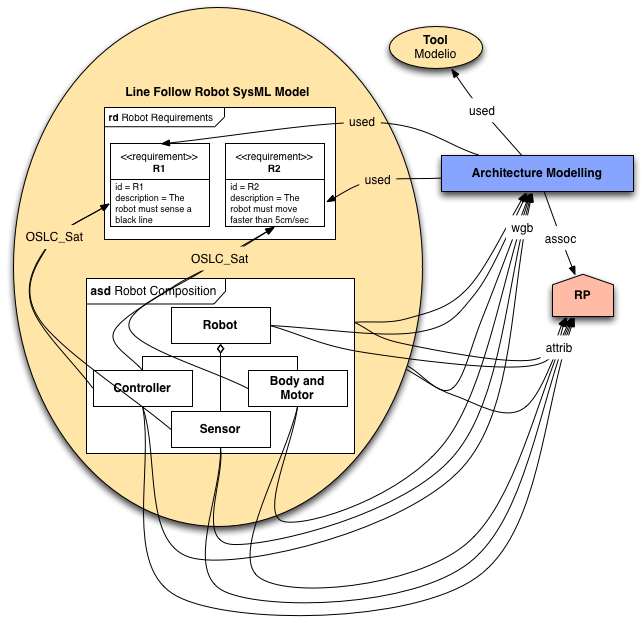
\includegraphics[width=0.8\textwidth]{figures/Traceability/step02}
\caption{Cross track error at various points for a robot trying to follow a desired line}\label{fig:crossTrackError}
\end{figure}

\draftnote{CJG: As the user(s) use the tools, they each record the their atomic actions, forming the traceability graph}

\draftnote{CJG: Give abstract view of a resulting trace}

\draftnote{CJG: A paragraph outlining the entities, activities and agents}

\section{Traceability Queries}

%\draftnote{TWT: FMU -> Requirements and Simulation Results -> FMUs are currently implemented.}

The traceability graph created by the INTO-CPS tool chain uses a graph database tool called \emph{Neo4J}. Once a graph has been built, queries can be executed over the graph to perform both forwards and backwards traceability. Below are some types of queries that can be executed over the graphs. The INTO-CPS Application supports some of these queries with the GUI, and the rest through inline access to the Neo4J console.

\begin{enumerate}[noitemsep]
  \item Impact analysis
  \begin{itemize}
    \item Forward traceability (from requirements to entities)
    \item Backwards traceability (from FMU to requirements)
    \item Backwards traceability (from components to requirements)
  \end{itemize}
  \item Simulation sources
  \begin{itemize}
    \item Find all simulations
    \item Find sources and sinks for a simulation
  \end{itemize}
  \item Coverage
  \begin{itemize}
    \item Requirements without architecture elements
    \item Requirements without simulation models
    \item Requirements without FMUs
    \item Requirements without positive simulation results
    \item Requirements without any simulation results
  \end{itemize}
  \item Code sources
  \begin{itemize}
    \item Find all generated source code entities
    \item Find the models for a given source code entity
  \end{itemize}
  \item User impact
  \begin{itemize}
    \item Find all users in the database
    \item Find all artefacts influenced by a user
    \item Find all activities performed by a user
  \end{itemize}
\end{enumerate}

Queries are written in Cypher, a query language built into Neo4J. Advanced users or those developing extensions to INTO-CPS can build their own queries in Cypher\footnote{\url{https://neo4j.com/developer/cypher-query-language/}} and execute them using Neo4J directly as described in the User Manual (Deliverable D4.3a~\cite{INTOCPSD4.3a}). 
\chapter{Requirements Engineering}
\label{sec:reqeng}

In this chapter, we consider the requirements engineering (RE) activities for the design of CPSs. Specifically, we consider the specification and documentation of requirements placed upon a CPS. These requirements may, for example, impose restrictions, define system capabilities or identify qualities of a system. The requirements should indicate some value or use for the different stockholders of a CPS.

As described in the previous chapter, traceability needs requirements to be defined as early as possible in a development process, and these must be recorded in Modelio for the machine-assisted traceability information to be recorded accurately. It is therefore appropriate to consider requirements processes for such developments at this stage.

In this remainder of this chapter, we discuss the needs for requirements engineering in CPS development, in particular based on the experience of the industrial partners for INTO-CPS. We describe one possible approach to RE for CPS, specifically adapting the SoS-ACRE approach for systems-of-systems (SoSs) to CPS. Note however that this approach is not mandatory, and in general RE processes and tools vary widely across organisations and domains. For this reason, tool support for traceability in INTO-CPS begins once requirements have been defined and can be added to Modelio. The diagrams described in the example are not part of INTO-CPS SysML specification. Therefore, this chapter should truly be treated as guidance, primarily serving to highlight the nature of RE for CPS, which may be of use for both new and more experienced CPS teams.

%In this project, we consider the state in the art of RE in both CPS and Systems of Systems (SoSs), reusing a previously defined approach to RE as applicable.

\section{Requirements Engineering and Cyber-Physical Systems}

The main issue of concern for RE in CPSs is that of differing domain contexts~\cite{Wiesner&14}. In addition, it has been noted that there are overlaps in challenges in CPSs and SoSs~\cite{Penzenstadler&12}--- especially independence, evolution and, increasingly, distribution. As described by Lewis et al.~\cite{Lewis&09}, as system architectures become more complex, there is often a need to consider requirements and structural architectures during the RE process. The authors suggest that an engineer should identify the system needs, component interactions and stakeholders, and map those needs onto those interested parties. %In Deliverable D3.1b~\cite{INTOCPSD31b}, we also surveyed several projects that had RE as a focus, or part of their focus.

As research in RE in CPS is a nascent field, we suggest one approach is to adopt RE processes from the SoS world, rather than defining an approach specifically for CPSs.  In chapter, we consider SoS-ACRE (System of Systems Approach to Context-based Requirements Engineering)~\cite{Holt&15}, as an example. This approach was adapted from standard systems engineering, and tailored for SoSs--- enabling the identification and reasoning about requirements across constituent systems of an SoS and understanding multi-stakeholder contexts. We suggest it might be useful to organisations trying to approach RE for CPS.

\section*{INTO-CPS industry partners and RE}

At the beginning of the INTO-CPS project, the four industrial partners were surveyed about their use of various technologies and methods, including requirements engineering~\cite{INTOCPSD31b}. Microsoft Excel was quoted as being used by three partners (UTRC, TWT and CLE), IBM Rational Doors used by one partner (UTRC), and Microsoft Word by one partner (AI).

Issues raised by industrial partners include:
\begin{itemize}
  \item Language/terminology of the requirements not consistent;
  \item Different people involved in the workflow do not have common understandings of requirements;
  \item Requirements traceability is considered to be highly inefficient and time consuming;
  \item Different people have to meet together and generate proofs among each other to validate dependable requirements; and
  \item Stakeholders do not have a clear vision about the product and tend to disagree on the objectives.
\end{itemize}

As can be seen, the above issues may be due to not having a rigorous RE approach, but also due to the challenges in CPSs--- that of different domains. In this section, we consider how a context-based approach to RE (SoS-ACRE) may be incorporated into the INTO-CPS tool chain, in particular using both the INTO-CPS technologies and the industrial partners' baseline technologies.

%%\fbox{check other sources for use on Excel in industry -- are industrial partners typical?}


\section{The SoS-ACRE View of Requirements}

We first consider the collection of views defined in SoS-ACRE, and their applicability to CPS engineering and the INTO-CPS tool chain. These views could be represented as diagrams in SysML\footnote{Note that SoS-ACRE is not specifically supported as a Modelio plug-in, but other equivalent diagrams could be used.}, or as we describe, could equally be represented in other tools where these are already used (e.g. Excel). Examples of each view are shown in Figures~\ref{fig:re-singlesysml}, \ref{fig:re-multisysml}, \ref{fig:re-uri-excel-sysml} and \ref{fig:re-excel-sysml}. %using  technologies relevant to INTO-CPS.

%\fbox{include example figures?}

\begin{description}
\item[Source Element View (SEV)] The SEV defines a collection of source materials from which requirements are derived. In SoS-ACRE, a SysML block definition diagram is considered. In INTO-CPS, this view could also be represented using an Excel table or Word document (with each source having a unique identifier), or by simply referring to source documents using OSLC traces.

\item[Requirement Description View (RDV)] The RDV is used to define the requirements of a system and forms the core of the requirement definition. SoS-ACRE suggests the use of SysML requirements diagram or in tabulated form, such as through the use of Excel. In addition, specifying requirements in  Doors would  support this view.

\item[Context Definition View (CDV)] The CDV is a useful view for CPS engineering in order to explicitly identify interested stakeholders and points of context in the system development, including customers, suppliers and system engineers themselves. In SoS-ACRE, they are defined using SysML block definition diagrams, and could also be represented using an Excel table or Word document (with each context having a unique identifier). This diagram type could be useful when identifying the divide in CT/DE and cyber-physical elements of a system.

\item[Requirement Context View (RCV)] In SoS-ACRE, a RCV is defined for each constituent system context identified in CDVs. This is appropriate when there is a set of diverse system owners, which is typical for SoSs and increasingly CPSs. A \textbf{Context Interaction View (CIV)} is then defined to understand the overlap of contexts and any common/conflicted views on requirements. In a CPS, however, there may not be such a clear delineation between the owners of constituent  system components. However, if we consider the different domains (e.g. CT/DE or cyber/physical divides) as different contexts, then this approach would be useful. In SoS-ACRE, RCVs and CIVs are both defined with SysML use case diagrams. Excel could be used if unique identifiers are defined for contexts and requirements as described earlier.

\item[Validation View (VV)] VVs, defined as SysML sequence diagrams in SoS-ACRE, describe validation scenarios for a SoS to ensure each constituent system context understands the correct role of the requirements in the full SoS. This is not an obvious fit in CPS engineering, and therefore not necessarily required.

\end{description}

\section{The SoS-ACRE RE Process}

The SoS-ACRE requirement engineering process may be useful for organisations wishing to better understand requirements for CPSm, particularly across multiple domains. It is a lightweight process, and therefore suitable for small- to medium-sized enterprises. Organisations with established may not feel the need to radically alter their existing practice, but may find it instructive to consider how their current processes might be updated or revised to consider better CPS requirements.

% The requirements management is considered to be too heavyweight a target for translation. This is largely due to the fact that we are currently less concerned with requirement change/different processes.

A SoS-ACRE process for CPS should include the following steps:

\begin{enumerate}
\item Identify and record source elements. This would be using a SEV, or simply recording paths to relevant files or documents.

\item Record system-level functional and non-functional requirements. Requirements may be derived using RDVs, and we could consider domain-specific requirements (e.g. cyber or physical), or analysis-specific requirement types (e.g. DSE or testing requirements).

\item Model initial System structure using INTO-CPS ASD. This will identify the cyber and physical elements and the domain/phenomena of the CPS. This may also give initial idea of component functionalities, which may lead to a repeat of Step 2 above\footnote{In the process of architectural modelling, it may also be necessary to redefine contexts depending on whether different simulation tools, or indeed different components of a model, are better able to provide the requirements of the CPS.}.

\item Define the various contexts in CDVs -- both external stakeholders, and if appropriate, contexts for the different components. If only a single system context is defined, then a single RCV is defined. However, if multiple contexts are defined for a CPS, then several RCVs are to be defined, along with a CIV to explore requirements from multiple contexts.

\item Trace the requirements through INTO-CPS tool chain models and results. This was covered in the previous chapter, however we revisit it below in the context of requirements.
\end{enumerate}

\section{Using technologies with SoS-ACRE}

%In this final section, we consider initial approaches to realise the relevant SoS-ACRE views using the INTO-CPS technologies and those used by industrial partners. This is not expected to constitute final guidelines on this area, as we would make use of INTO-CPS technology currently in development -- namely traceability and provenance support.

As INTO-CPS does not specifically support SoS-ACRE. Indeed INTO-CPS does not mandate and specific approach to RE, because of the wide variety of approaches in industry. We conclude this chapter with an example of how a SoS-ACRE (or other RE process) could be integrated into an INTO-CPS development. We describe a range of permutations of the use of models and documents for recording the requirements engineering process described above. In addition, we include discussions on the links between requirements and architectural models--- identified above as a key method for requirements engineering in CPSs. %We also refer to OSLC and Prov links, which could be linked into the INTO-CPS traceability, though are not supported by the tool chain at the end of the project. Further information on OSLC can be found in Deliverable D3.3b~\cite{INTOCPSD3.3b}.

\begin{description}

\item[URI, Excel and SysML]

We first consider an approach using URIs for the source elements, an Excel document (or a collection of Excel tables) for the RDV, CDV, RCV and CIV of SoS-ACRE. A SysML model in Modelio can be used to define the architecture of the multi-model. Internal tracing in Excel can be achieved using identifiers referenced between sheets. Excel requirements can be replicated in Modelio then traced to elements in the INTO-CPS tool chain automatically. Figure~\ref{fig:re-uri-excel-sysml} presents an example with URI, Excel and SysML models and OSLC links between the artefacts.

\item[Excel and SysML]

The next approach uses Excel to define the SEV and RDV of SoS-ACRE, a SysML model to define the context-oriented views (CDV, RCV and CIV) and a separate architectural model to define the CPS architecture. The Excel requirements can then be mirrored in a Modelio model, and linked to the architectural model. The INTO-CPS traceability features can trace the requirement artefacts to the architectural model. Additional OSLC links could be added manually to link elements of the Excel requirements and context views in a SysML.  Figure~\ref{fig:re-excel-sysml} presents an example with URI, Excel and two SysML models with OSLC links between the artefacts.

\item[Single SysML model]

The next permutation is to use a single SysML model for both requirements engineering and architectural modelling. Such a model will contain all SoS-ACRE views\footnote{Note that Modelio does not currently provide an extension for SoS-ACRE, but these views can be realised using existing SysML stereotypes.} (SEV, RDV, CDV, RCV and CIV), in addition to diagrams defined using the INTO-CPS profile for the CPS composition and connections. Modelling in this way enables trace links to be defined inside a single SysML model. Figure~\ref{fig:re-singlesysml} presents an example SysML model with trace relationships.



\item[SysML requirements and SysML architectural models]

The final permutation is to use SysML for both requirements engineering and architectural modelling, however to use two separate models for the two activities (one containing the RE views (SEV, RDV, CDV, RCV and CIV) and another for architectural diagrams (ASD and CD)). We consider this permutation with two SysML models in addition to the single SysML model, because the requirements engineering and architectural modelling activities are often considered separately, with different engineering teams comprised of engineers with specialist skills. As such we can assume there are cases where these teams have ownership of different models.
Trace links may be used within each individual model (for example, tracing from source elements to requirements in a RE model), and OSLC links defined to trace between requirements elements and architectural elements. Figure~\ref{fig:re-multisysml} presents an example with two SysML models with trace relationships and OSLC links between the models.

\begin{figure}
	\centering
	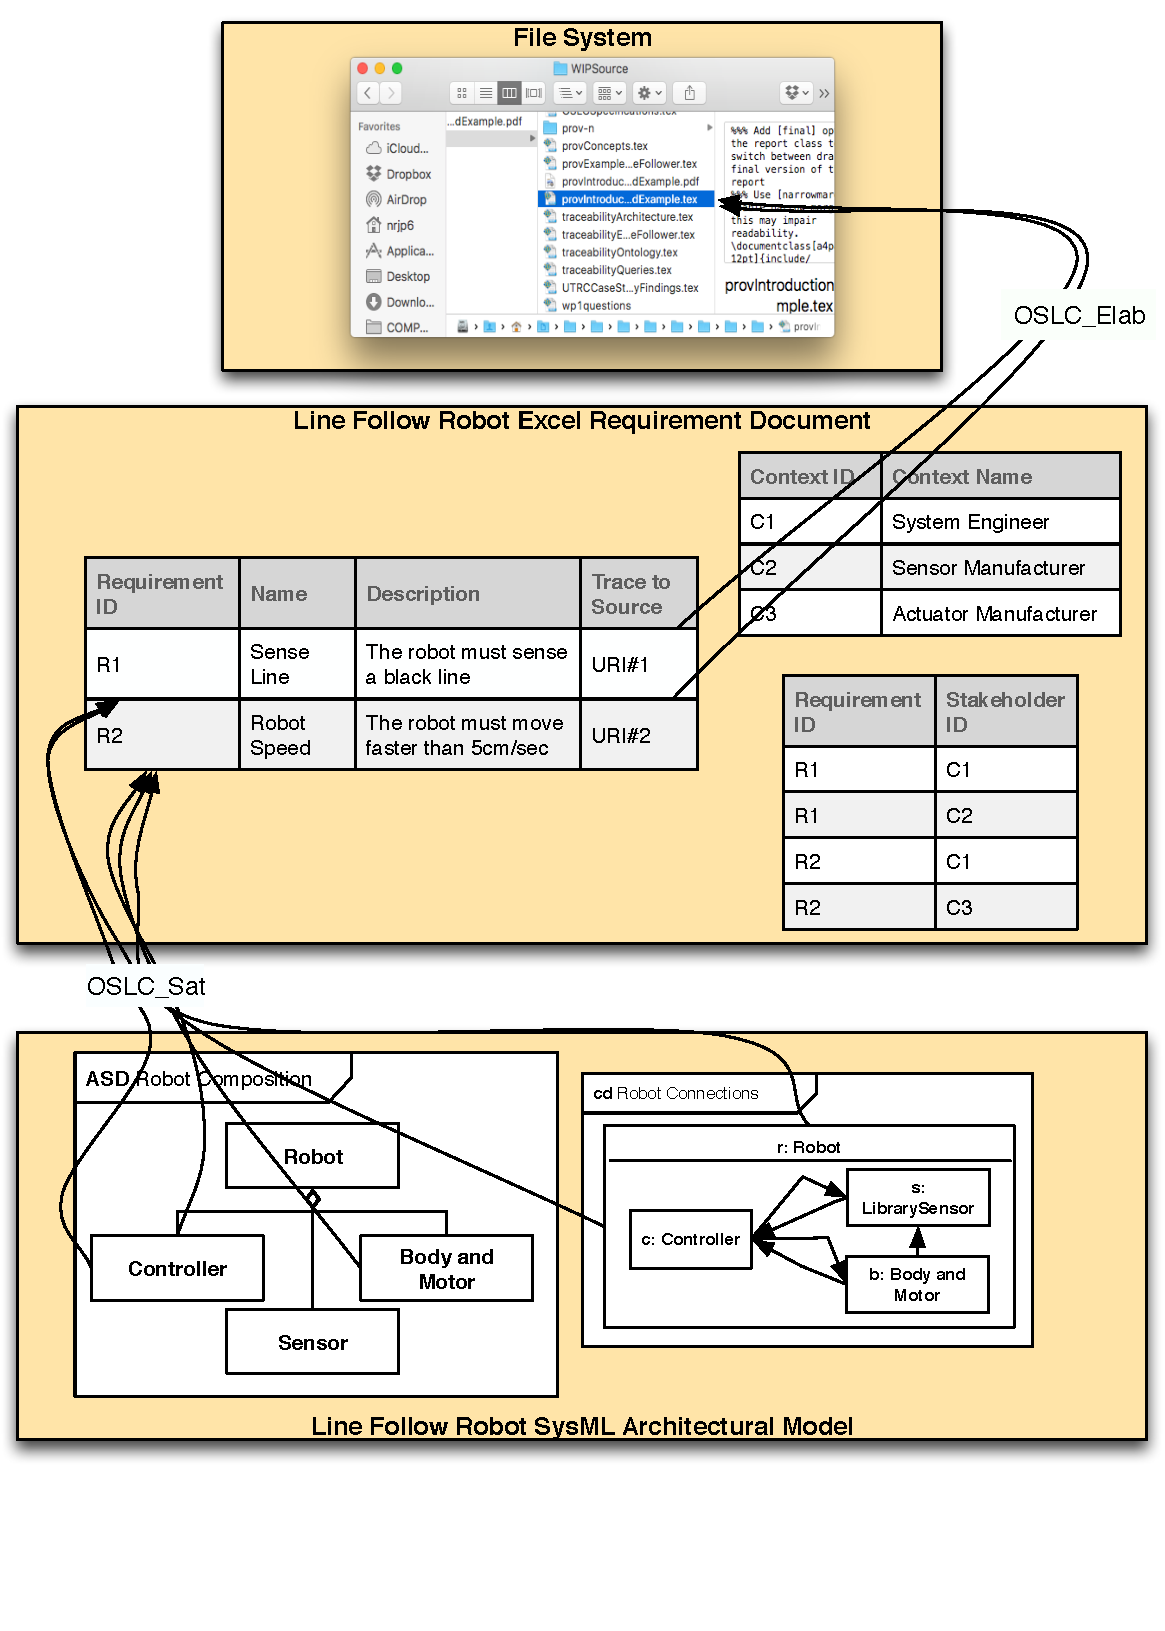
\includegraphics[scale=0.65]{figures/RE_3}
\caption{URI, Excel and SysML -- model overview}
\label{fig:re-uri-excel-sysml}
\end{figure}

\begin{figure}
	\centering
	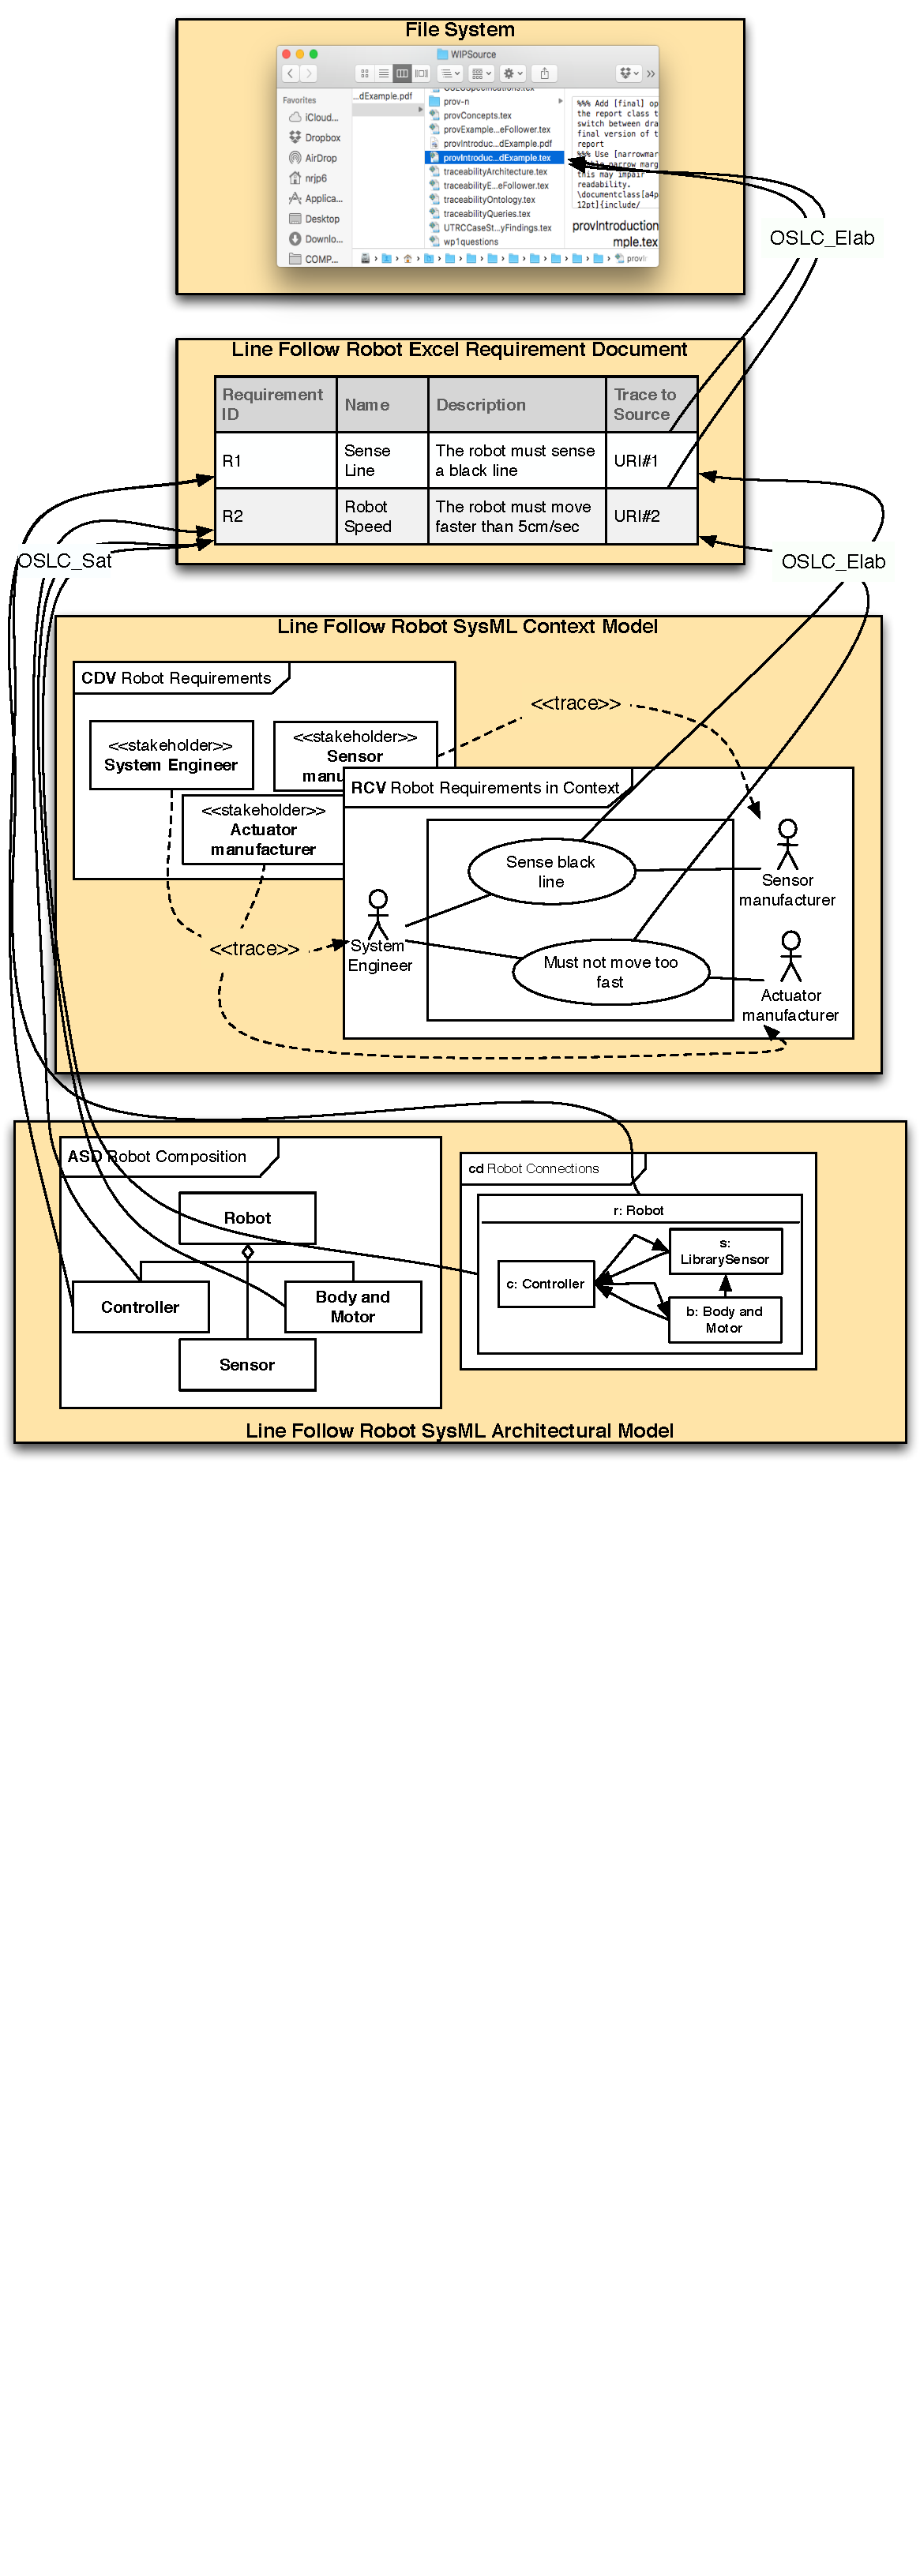
\includegraphics[width=0.8\textwidth]{figures/RE_4}
\caption{Excel and SysML -- model overview}
\label{fig:re-excel-sysml}
\end{figure}

\begin{figure}
	\centering
	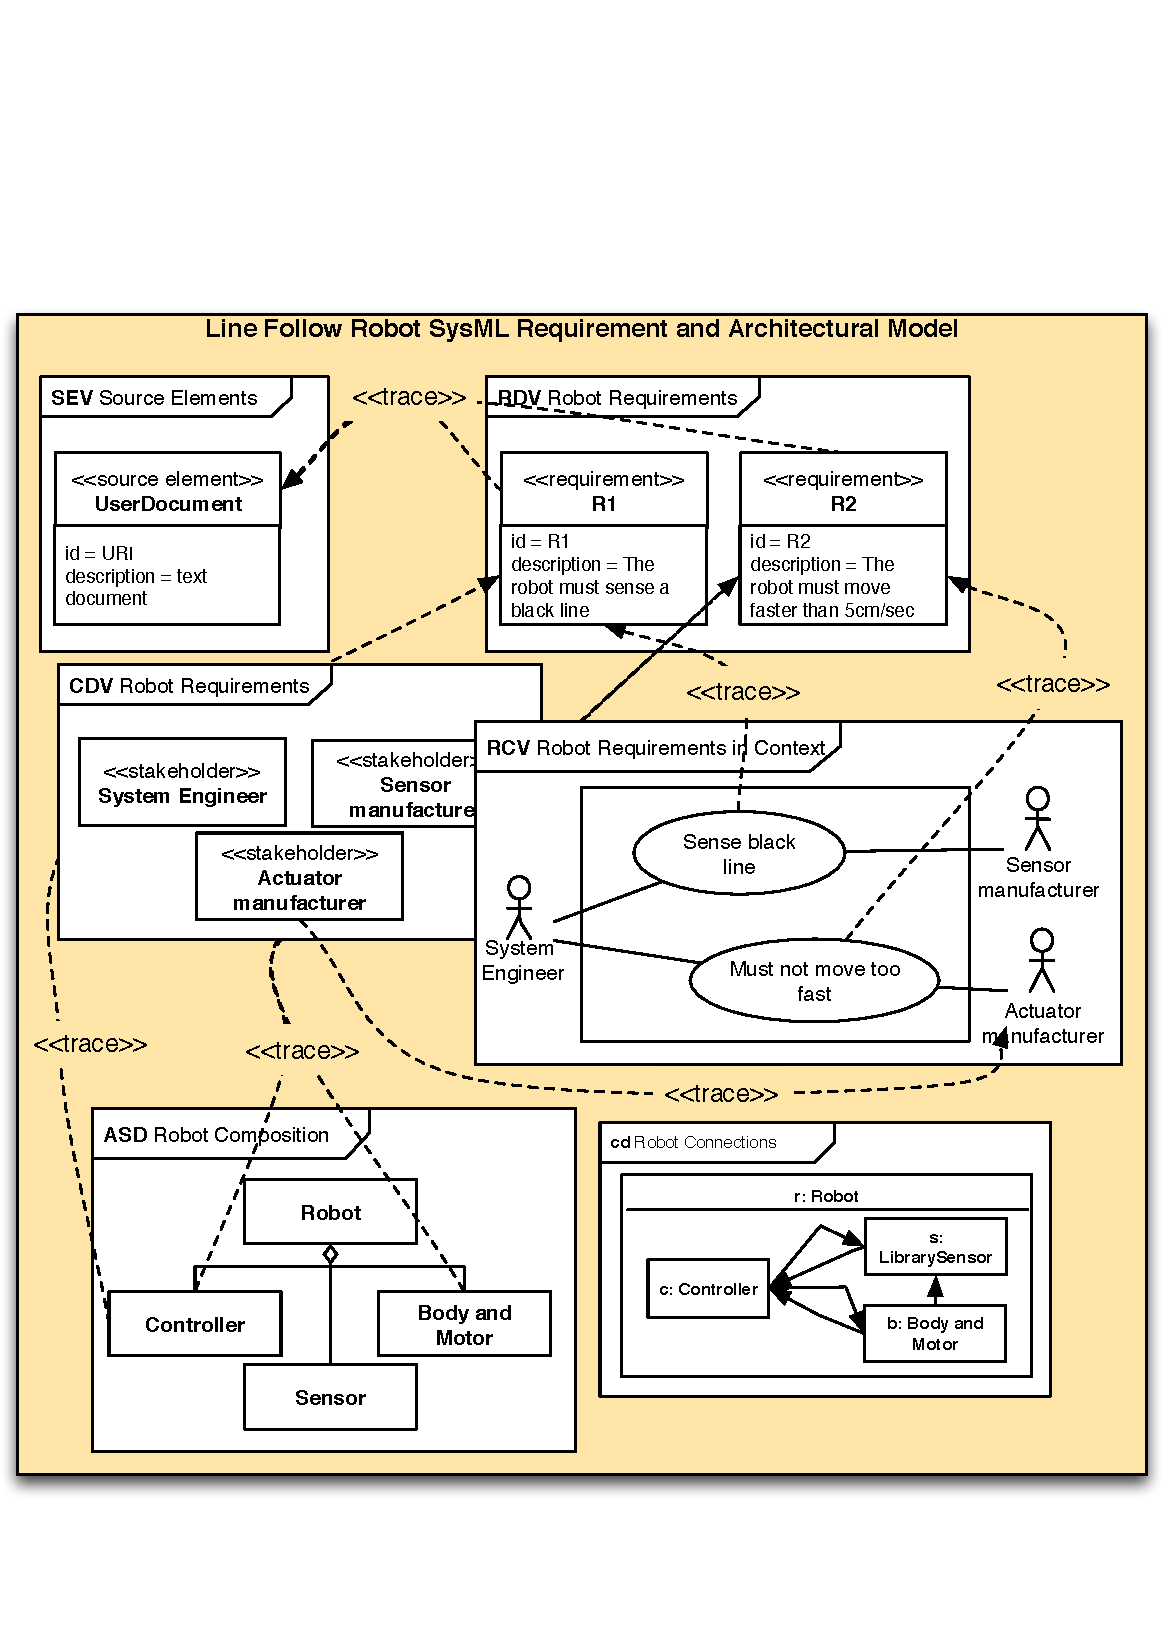
\includegraphics[scale=0.7]{figures/RE_1}
\caption{Single SysML model -- model overview}
\label{fig:re-singlesysml}
\end{figure}

\begin{figure}
	\centering
	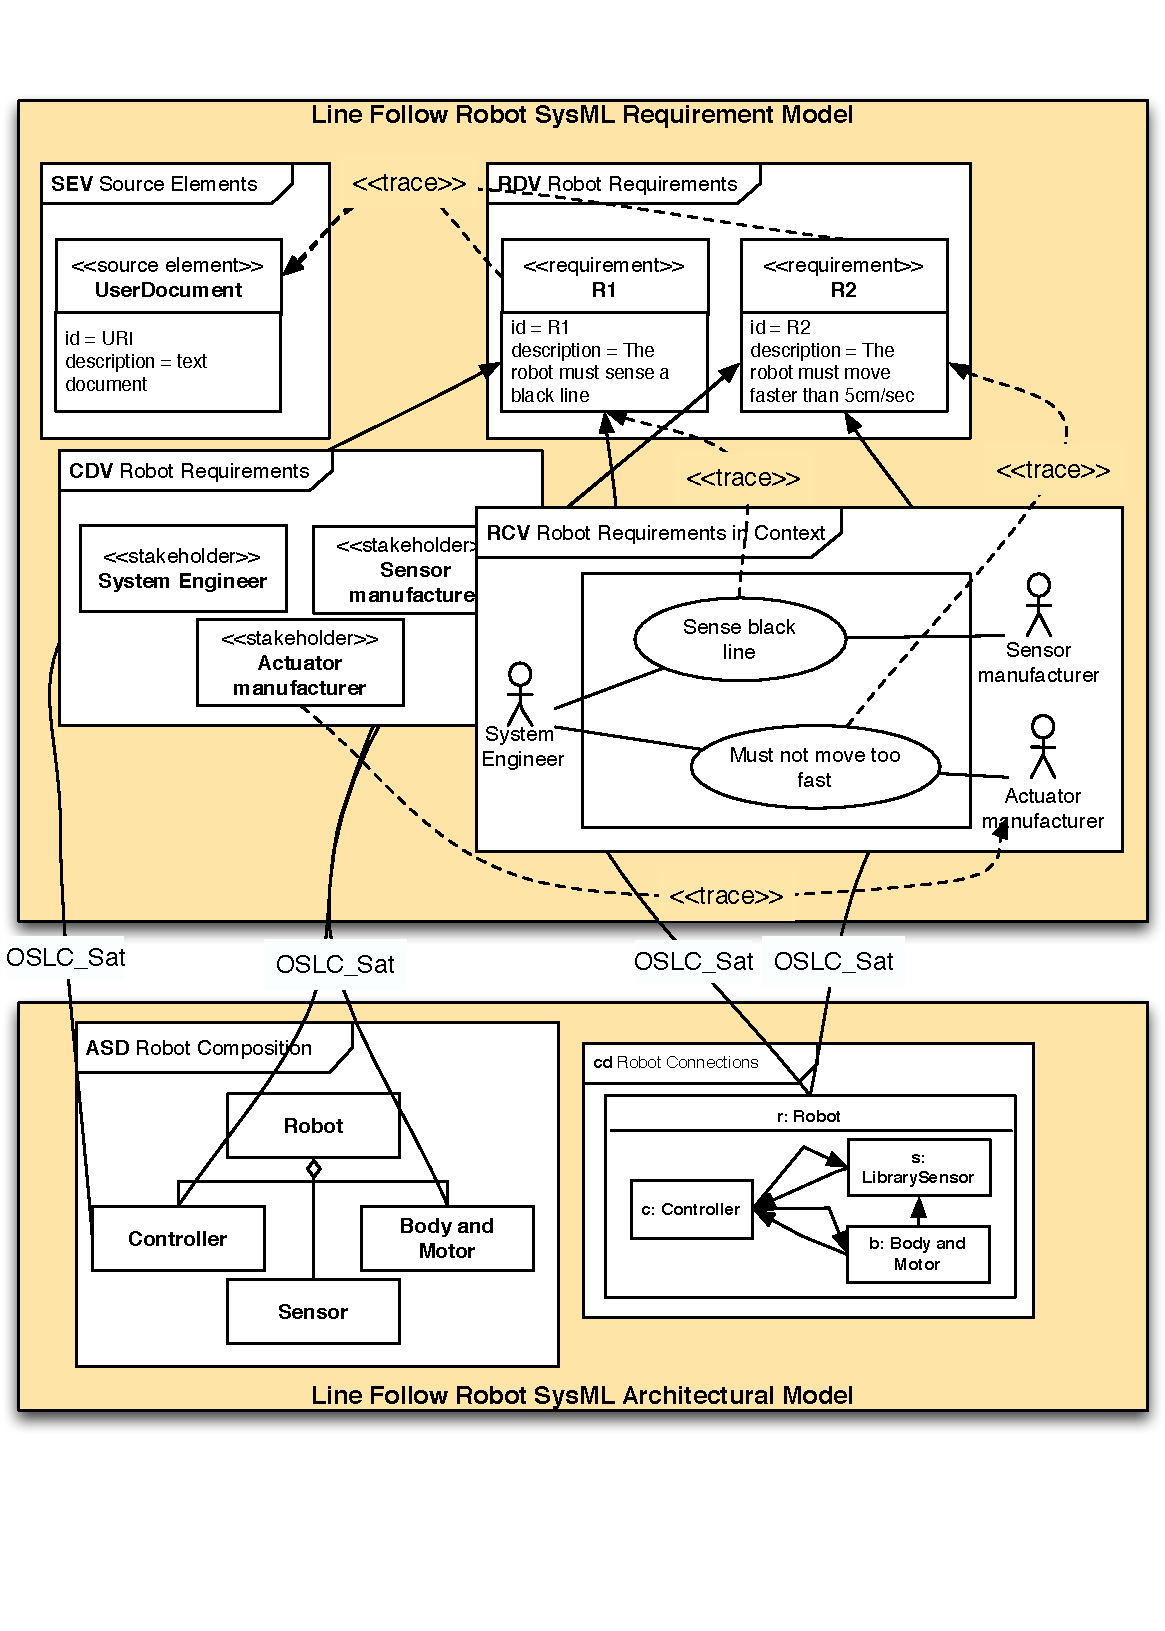
\includegraphics[scale=0.7]{figures/RE_2}
\caption{SysML requirements and SysML architectural models -- model overview}
\label{fig:re-multisysml}
\end{figure}
\end{description}

%
% MOVED TO FINAL CHAPTER
%

%\section{Future Guidelines}
%
%In the final year of the INTO-CPS project, we will consider additional guidelines in RE--- specifically regarding links from requirements to modelling for analysis  and to the analysis results themselves. For example, we would consider guidelines for specifying requirements that influence objectives defined in design space exploration. This is alluded to in Section~\ref{sec:dse-linefollow}. We shall also consider how this relates to co-simulation and the existing work in test automation -- as reported in Deliverable D5.1b~\cite{INTOCPSD51b}.

\chapter{SysML and Multi-modelling}
\label{sec:sysml}

This chapter describes the use of SysML with the INTO-CPS tool chain. As described previously in Chapter~\ref{sec:reqeng}, standard SysML can be used as part of a development process to build a model of a system and link elements to requirements. The INTO-CPS tool chain also provides an extended SysML profile that help users to \emph{configure multi-models for co-simulation} and \emph{configure design space exploration (DSE) analysis}~ ~\cite{INTOCPSD2.1a,INTOCPSD2.2a,INTOCPSD2.3a,INTOCPSD41c,INTOCPSD4.2c,INTOCPSD4.3c}. For ease explanation, we describe these separately below, however all the diagrams described are part of a single extended SysML profile.

This chapter summarises the diagrams provided in the two profiles and describe their use in Sections~\ref{sec:sysml:intocps} and~\ref{sec:sysml:dse}. The diagrams presented are illustrative, showing the main elements of a diagram; they are not full definitions of the meta-model, which can be found in the documents cited above. All diagrams are supported by the Modelio tool, and we refer readers to the user manual, Deliverable D4.3a~\cite{INTOCPSD4.3a}, for further information on how to use Modelio to draw these diagrams and generate configurations for use in the INTO-CPS Application.

The chapter concludes with an example of the relationship between a \emph{holistic} model created using standard SysML and a \emph{design} model using the INTO-CPS profile, and concludes with a discussion on how to represent non-design elements (such as FMUs that only perform visualisation) in the INTO-CPS profile in Section~\ref{sec:sysml:non-design}.

\section{SysML Diagrams Describing Multi-models}
\label{sec:sysml:intocps}

The multi-modelling SysML profile defines two diagrams for configuring a co-simulation. The INTO-CPS Application can run a co-simulation based on a configuration file, using the JSON format to describe the FMUs, their parameters and connections between them. These can be created manually in a text editor, or from the INTO-CPS Application itself. Alternatively, a configuration can be generated by Modelio from the diagrams defined in this profile. There are two types diagram, the \emph{Architectural Structure Diagram} describing the static structure of FMUs, and the \emph{Connections Diagram} describing their instantiation and connections. These are shown in Figure~\ref{fig:sysml:intocps}.

\begin{figure}[h!]
\centering
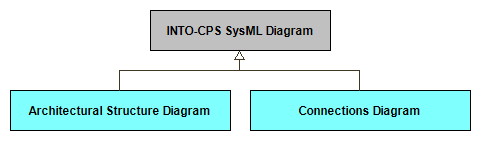
\includegraphics[scale=0.6]{figures/Architecting/ArchitecturalViews}
\caption{Diagrams in the multi-modelling SysML profile}
\label{fig:sysml:intocps}
\end{figure}

\newpage
\subsection{Architectural Structure Diagram}
\label{sec:sysml:intocps:asd}

The \emph{Architecture Structure Diagram} (ASD) specialises SysML block definition diagrams (BDDs) to support the specification of a multi-model architecture described in terms of a systems components, which will be represented by FMUs. As shown in Figure~\ref{fig:sysml:sysml:intocps:ase} this diagram must include a \texttt{<<System>>} which is then broken down into zero or more \texttt{<<Component>>} blocks.

\begin{figure}[h!]
\centering
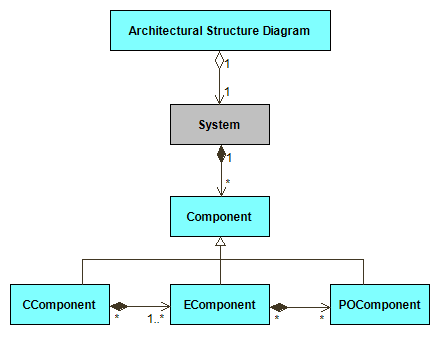
\includegraphics[scale=0.6]{figures/Architecting/ArchitecturalStructureElements}
\caption{\emph{Architectural Structure Diagram} describing FMUs (EComponents) and their hierarchies}
\label{fig:sysml:sysml:intocps:ase}
\end{figure}

There are three types of component block. The \texttt{<<EComponent>>} (encapsulating component) represents a part of a system that will be represented by a single FMU. These blocks have properties indicating which modelling language and tool will be used: \texttt{modelType} (\emph{discrete} or \emph{continuous}) and \texttt{platform} (\emph{VDMRT}, \emph{TwentySim}, \emph{OM}, and \emph{other}).

An \texttt{<<EComponent>>} can be broken down logically into \texttt{<<PComponent>>} (part-of component) representing an internal element of an \texttt{<<EComponent>>}. Both \texttt{<<EComponent>>} and \texttt{<<PComponent>>} blocks can define \emph{variables} and \emph{FlowPorts} that an FMU will have.

The third type of component is a \texttt{<<CComponent>>} (collection component) that allows other components to be grouped logically (it has no ports or behaviours). These can be used to separate design elements within a diagram, as described in Section~\ref{sec:sysml:non-design}. All component blocks have a \emph{kind} that marks their purpose in the model (\emph{cyber}, \emph{physical}, \emph{environment}, \emph{visualisation}).

FMUs are connected by \emph{ports}, and may also present internal state through externally visible \emph{variables}, which can be monitored on a live graph, for example. Both \texttt{<<EComponent>>} and \texttt{<<PComponent>>} blocks can define \emph{FlowPort} and \emph{Variable} attributes, as shown in Figure~\ref{fig:sysml:sysml:intocps:asi}, which will form the interface of the FMU and are added to the ``model description'' exported by Modelio.

\begin{figure}[h!]
\centering
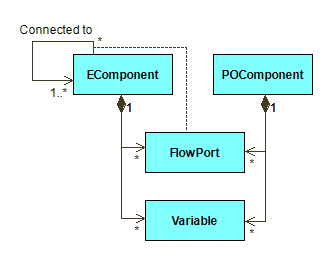
\includegraphics[scale=0.6]{figures/Architecting/ArchitecturalStructureInterfaces}
\caption{Component blocks may define variables and ports}
\label{fig:sysml:sysml:intocps:asi}
\end{figure}

%\begin{figure}[h!]
%\centering
%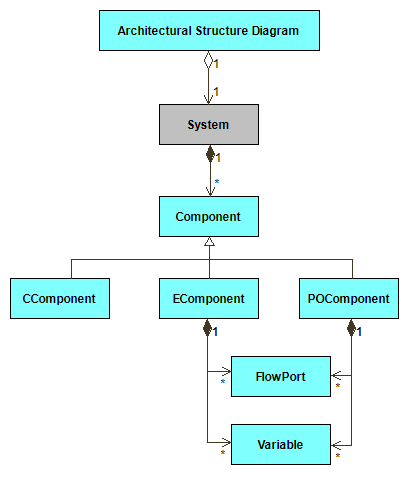
\includegraphics[scale=0.6]{figures/Architecting/ArchitecturalStructureView}
%\caption{\emph{Architectural Structure Diagram} describing connections between FMUs}
%\label{fig:sysml:sysml:intocps:asd}
%\end{figure}

%\clearpage
\subsection{Connections Diagram}
\label{sec:sysml:intocps:cd}

The \emph{Connections Diagram} (CD) specialises SysML internal block diagrams to convey the internal configuration of the systems components. Specifically, it describes which FMUs are instantiated (i.e. which \texttt{<<EComponent>>}s form the ASD), and how the ports are connected. This diagram is used by Modelio to generate multi-model configurations.

\begin{figure}[h!]
\centering
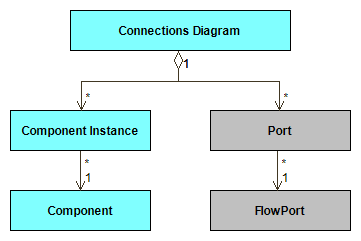
\includegraphics[scale=0.6]{figures/Architecting/ConnectionsView}
\caption{\emph{Connections Diagram} describing the static structure of FMUs}
\label{fig:sysmlintocps:cd}
\end{figure}

\section{SysML Diagrams Describing Design Space Exploration}
\label{sec:sysml:dse}

The design space exploration (DSE) SysML profile is an addition to the multi-modelling SysML profile described above. As with single co-simulation, the INTO-CPS Application can run a DSE based on a JSON configuration file. These can be created manually in a text editor or edited in the INTO-CPS Application. Alternatively, a configuration can be generated by Modelio, from a set of diagrams defined in the profile. There are five diagram types, which are described below. Further guidance on DSE can be found in Chapter~\ref{sec:dse}.

\begin{figure}[h!]
\centering
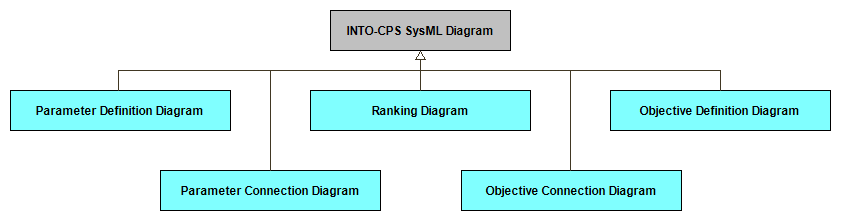
\includegraphics[scale=0.5]{figures/DSE/DSEViews}
\caption{Diagrams in the DSE SysML profile}
\label{fig:sysml:dse}
\end{figure}

\subsection{Objective Definition Diagram}
\label{sec:sysml:dse:odd}

The \emph{Objective Definition Diagram} is used to define the objectives for use during a DSE. Objectives are characterising measures of performance that may be used to determine the relative benefits of competing designs. They are defined as metrics over the results of a co-simulation of a specific design and are used to judge its quality for use in later processing e.g. ranking.

Objectives are described in terms of a name, a script file that will be used to compute them, and the ports that will provide the data they require. As with the \emph{Architectural Structure Diagram} above (Section~\ref{sec:sysml:intocps:asd}), this diagram gives the static structure of the objectives; instances of these definitions are created using the \emph{Objective Connection Diagram} below (Section~\ref{sec:sysml:dse:ocd}).

\begin{figure}[h!]
\centering
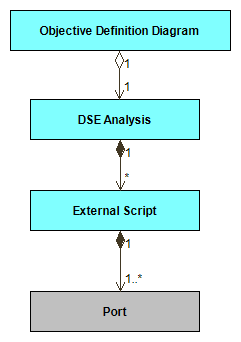
\includegraphics[scale=0.5]{figures/DSE/ObjectiveDefinitionView}
\caption{\emph{Objective Definition Diagram} describing objectives in a DSE}
\label{fig:sysml:sysml:dse:odd}
\end{figure}

\subsection{Objective Connection Diagram}
\label{sec:sysml:dse:ocd}

The \emph{Objective Connection Diagram} is used to instantiate objectives defined in the \emph{Objective Definition Diagram} above (Section~\ref{sec:sysml:dse:odd}). The diagrams allow the ports of each instance of the objective to be linked to a data source: either a static value, or a value from data exchanged in the multi-model.

\begin{figure}[h!]
\centering
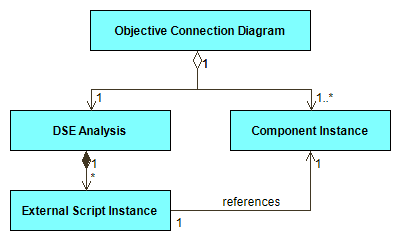
\includegraphics[scale=0.5]{figures/DSE/ObjectiveConnectionsView}
\caption{\emph{Objective Connections Diagram} linking objectives to data sources}
\label{fig:sysml:sysml:dse:ocd}
\end{figure}

\subsection{Parameter Definition Diagram}
\label{sec:sysml:dse:pdd}

The \emph{Parameter Definition Diagram} is used to define the parameters that will changed for each co-simulation in a DSE. Parameters are described in terms of a name, and a set of values that we wish to test. The product of the cardinalities of the set of values for each parameter gives the size of the design space--- the total number of simulation required for an exhaustive search. As with the \emph{Architectural Structure Diagram} above (Section~\ref{sec:sysml:intocps:asd}), this diagram gives the static structure of the parameters; instances of these definitions are created using the \emph{Parameter Connection Diagram} below (Section~\ref{sec:sysml:dse:pcd}).

\begin{figure}[h!]
\centering
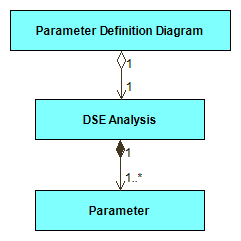
\includegraphics[scale=0.5]{figures/DSE/ParameterDefinitionView}
\caption{\emph{Parameter Definition Diagram} defining parameters and their values}
\label{fig:sysml:sysml:dse:pdd}
\end{figure}

\subsection{Parameter Connection Diagram}
\label{sec:sysml:dse:pcd}

The \emph{Parameter Connection Diagram} is used to instantiate parameters defined in the \emph{Parameter Definition Diagram} above (Section~\ref{sec:sysml:dse:pdd}). The diagram allows the parameters to be linked to those provided by the FMUs in the multi-model.

\begin{figure}[h!]
\centering
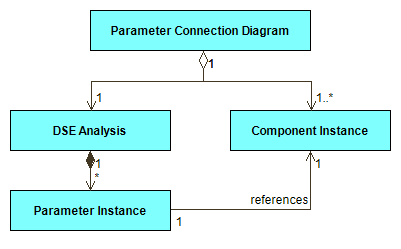
\includegraphics[scale=0.5]{figures/DSE/ParameterConnectionsView}
\caption{\emph{Parameter Connections Diagram} linking parameters to FMUs}
\label{fig:sysml:sysml:dse:pcd}
\end{figure}

\subsection{Ranking Diagram}
\label{sec:sysml:dse:rd}

The \emph{Ranking Diagram} is used to declare which of the objectives should be used to compare competing designs, and whether lower or higher values for each the objectives is better (i.e. whether to maximise or minimise a value).

\begin{figure}[h!]
\centering
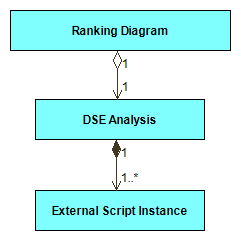
\includegraphics[scale=0.5]{figures/DSE/RankingView}
\caption{\emph{Ranking Diagram} defining how to rank designs based on objectives}
\label{fig:sysml:sysml:dse:rd}
\end{figure}


\section{Holistic and Design Architectural Modelling}
\label{sec:sysml:holistic}

A system architecture defines the major components of a system, and identifies their relationships, behaviour and interactions. A model of the architecture is potentially partial (representing some or all of the system) and abstract, limited to those elements pertinent to the modelling goal. In CPS engineering, this goal may include understanding the system in terms of the application domain (a \emph{holistic} model), or capturing the system components in a way that targets multi-modelling (a \emph{design} model).

The diagrams in the two profiles described above divide architectural models into subsystems composed of cyber or physical components. Defining an architecture this way may not be the best approach when designing a system ab initio, with systems comprising entities across different domains requiring diverse domain expertise. Following on from Chapter~\ref{sec:reqeng}, this section uses a smart grid example to show both holistic and design architectural modelling approaches, and provide some commentary and guidance on how to model in a way which is natural for domain experts, and how to move from holistic to design models when multi-modelling.

\subsection*{Example Introduction}

%\fbox{mention what a SG is briefly:  control, distributed control, ideas of power gen, transmission, substations etc}
A smart grid is an electricity power grid where integrated ICT systems play a role in the control and management of the electricity power supply. Such ICT elements include distributed control in households, control of renewable energies and networked communications.
In this section we outline a Smart Grid\ model to explore different design decisions in the cyber control of an electricity power grid. The model presented here is a small illustrative example, which omits complexities of a real Smart Grid. For example, the change from three-phase AC power to one-phase DC power allowing us to use simpler physical models. A second simplification is in the number of houses present in the grid model. We model only 5 houses, assumed to be in a small local area supplied by a single substation. We do not consider the remainder of the grid. To ensure that any effect due to changes in the power consumption by those properties are observed by the other houses, we skew the resistance of the transmission lines between the power generation and substation, and substation to houses.

\subsection*{Holistic Architectural Model}

A Block Definition Diagram (BDD) of the Smart Grid is given in Figure~\ref{fig:bdd}. The figure shows that the \textit{Smart Grid} system comprises two top-level physical elements: \textit{Power Generation} and \textit{Transmission Lines}; a single top-level cyber elements: the \textit{Data Network}; and two cyber-physical systems: a \textit{Substation} and several \textit{Houses}. The two elements may be further decomposed. The \textit{Substation} elements is composed of a cyber \textit{Substation Controller} and physical \textit{Substation Meter} and \textit{Step-down Transformer}. The \textit{House} element comprises: a cyber \textit{House Controller}, physical \textit{House Meter} and \textit{Devices}, and an \textit{Owner/Usage Profile}.

\begin{figure}
\centering
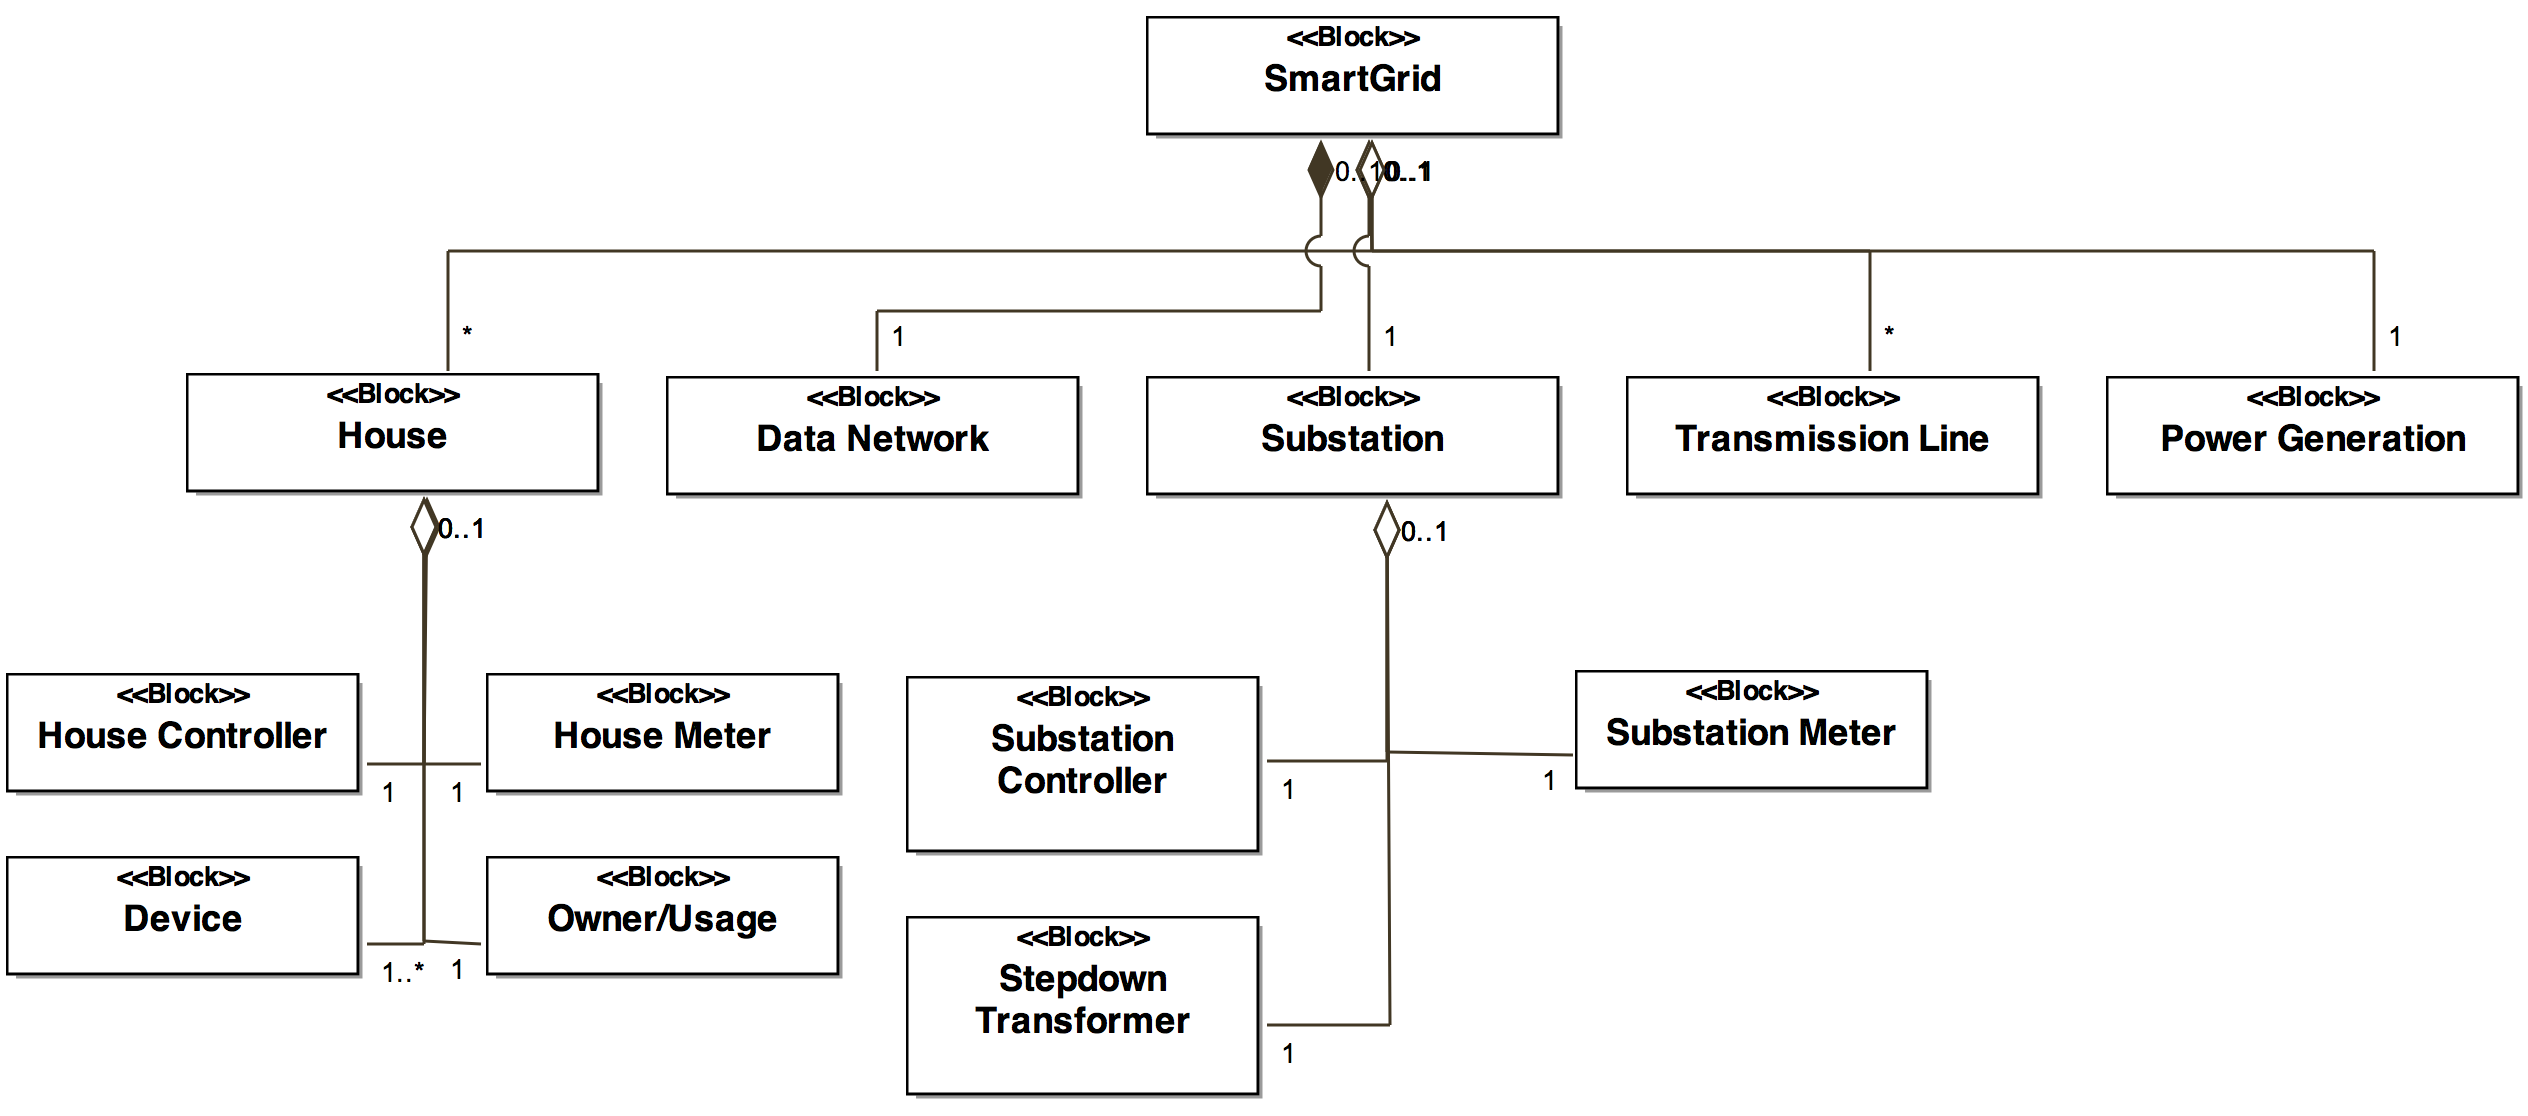
\includegraphics[width=1\textwidth]{figures/BDDSmartGrid}
\caption{Block Definition Diagram of Smart Grid}
\label{fig:bdd}
\end{figure}

An Internal Block Diagram (IBD) of the Smart Grid is given in Figure~\ref{fig:ibd}. The diagram shows there are two main connection types in the model, corresponding to the physical power connections and the cyber data connections. The model also shows the connections between the cyber and physical parts of the models -- currently modelled using data-type connections.

\begin{figure}
\centering
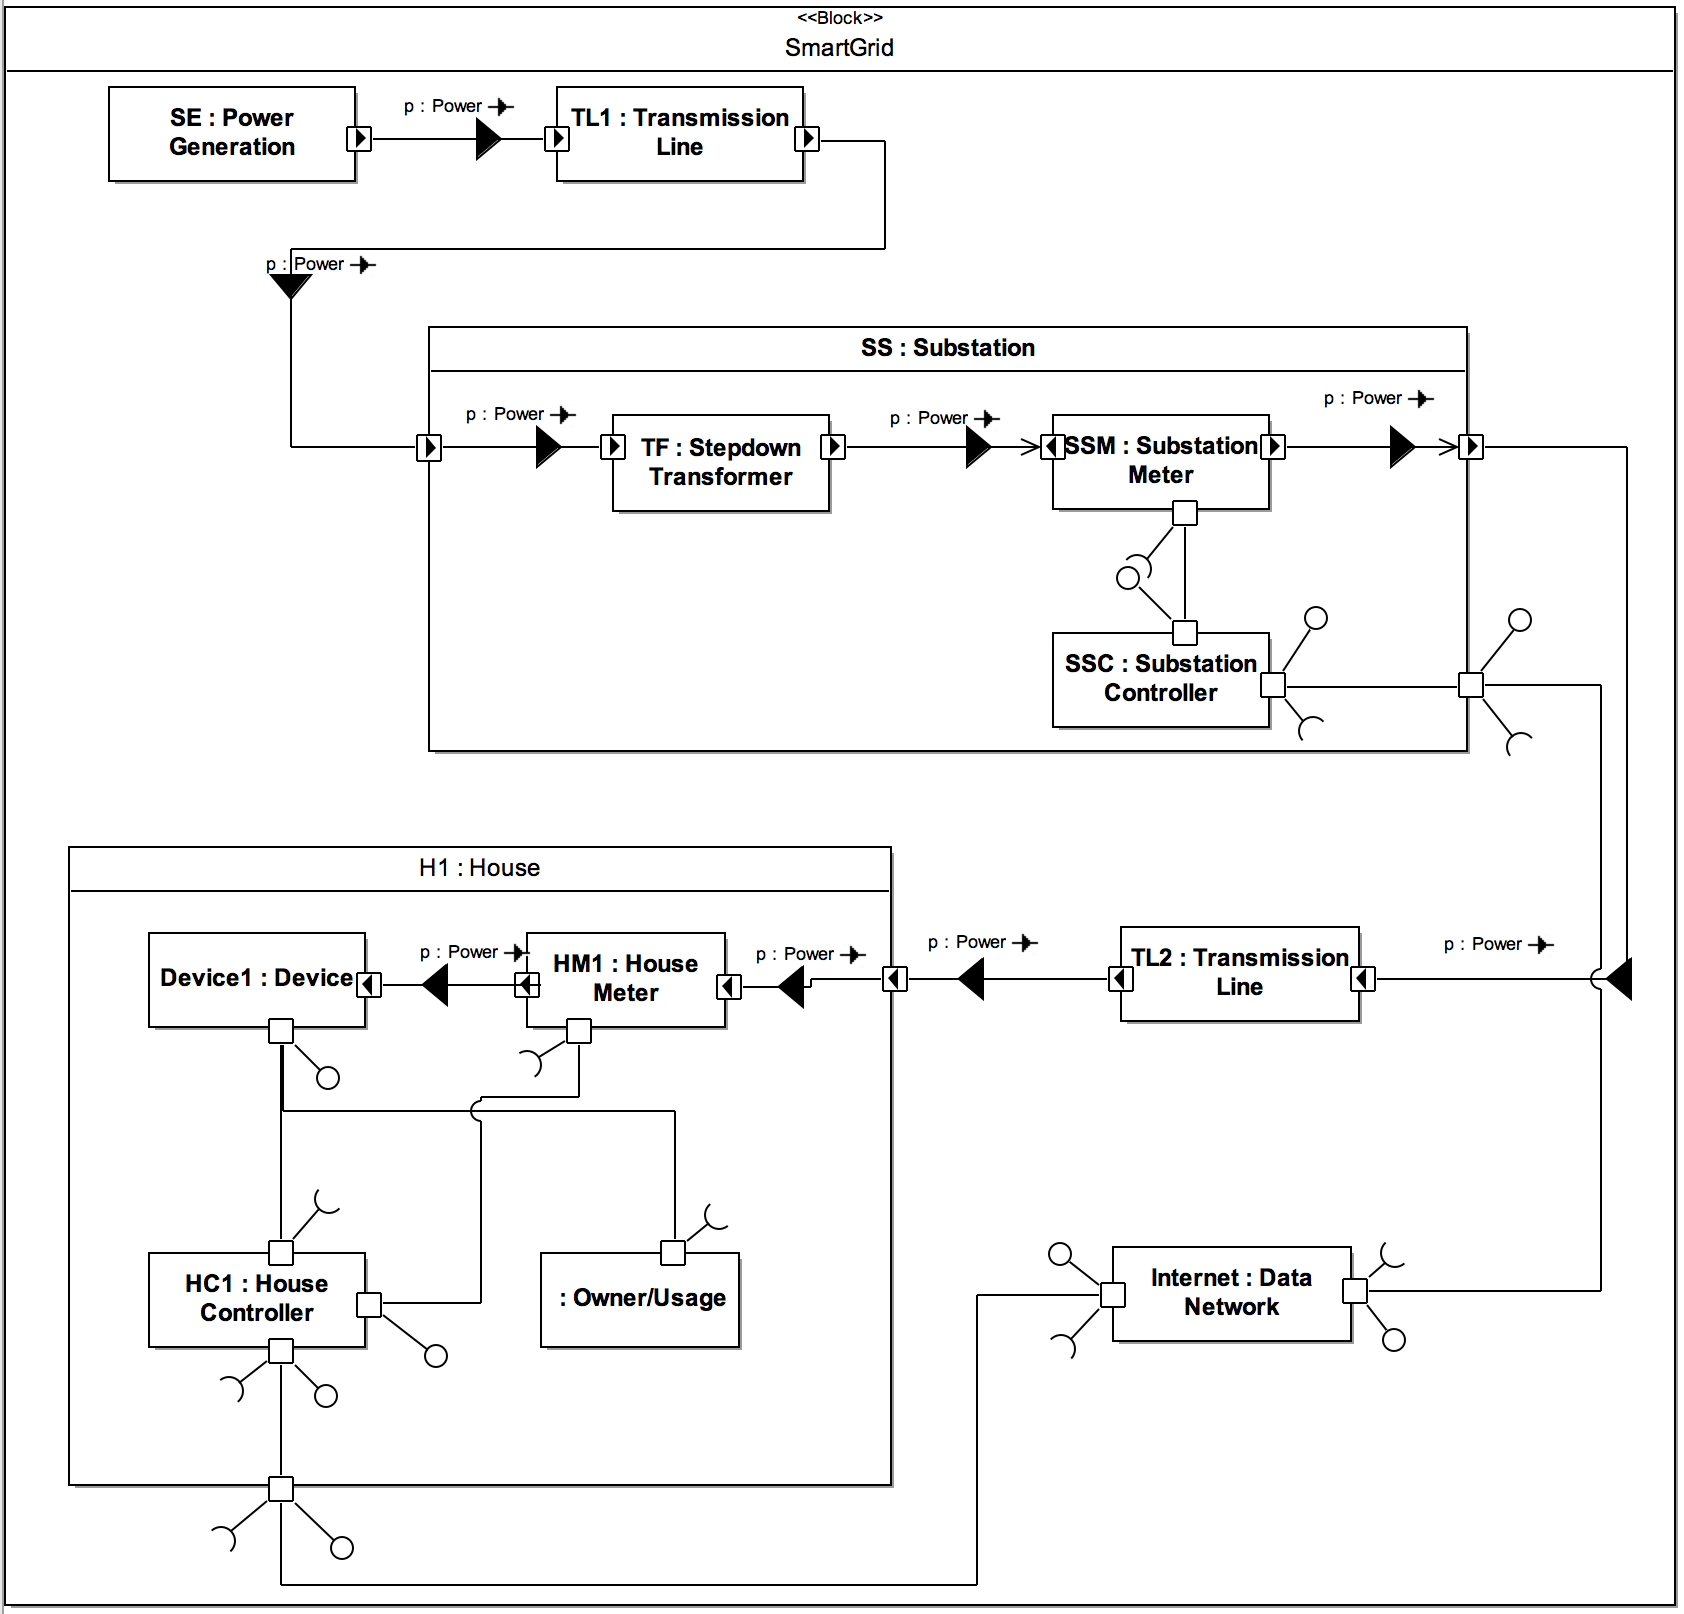
\includegraphics[width=0.85\textwidth]{figures/IBDSmartGrid}
\caption{Internal Block Diagram of Smart Grid}
\label{fig:ibd}
\end{figure}

The first type of connection ---the physical power connections--- show a flow of \textit{Power} from the Power Generation, through the Transmission Lines to the Houses, via the Substation. In the Substation, the Stepdown Transformer is connected to the Substation Meter. Similarly, in each House (only one is shown in the figure), the Power flows through the House Meter to each Device (again only one is shown for readability). The data connections exist between the Substation Controller and House Controllers. The Data Network is explicitly modelled and links the various controllers. Finally, there are links between the cyber controllers and the physical systems. In this model, the Substation Controller is connected to the Substation Meter, and the House Controller is linked to the House Meter and Devices.

\subsubsection*{Design Architectural Model}

% KGP: So actually we could update this to use CComponents to ``better reflect the holistic architecture''?

Looking at the holistic architecture defined in Figures~\ref{fig:bdd} and~\ref{fig:ibd} and moving towards a multi-model, we use the INTO-CPS SysML profile to define the architecture of the Smart Grid\ from the perspective of multi-model. This yields the ASD in Figure~\ref{fig:asd_mm}. This structure removes all subsystem structures such that each component is to be realised in a single FMU. Each element is defined as either a \emph{physical} or \emph{cyber} component, with the model type and platform identified.

\begin{figure}[htbp]
\centering
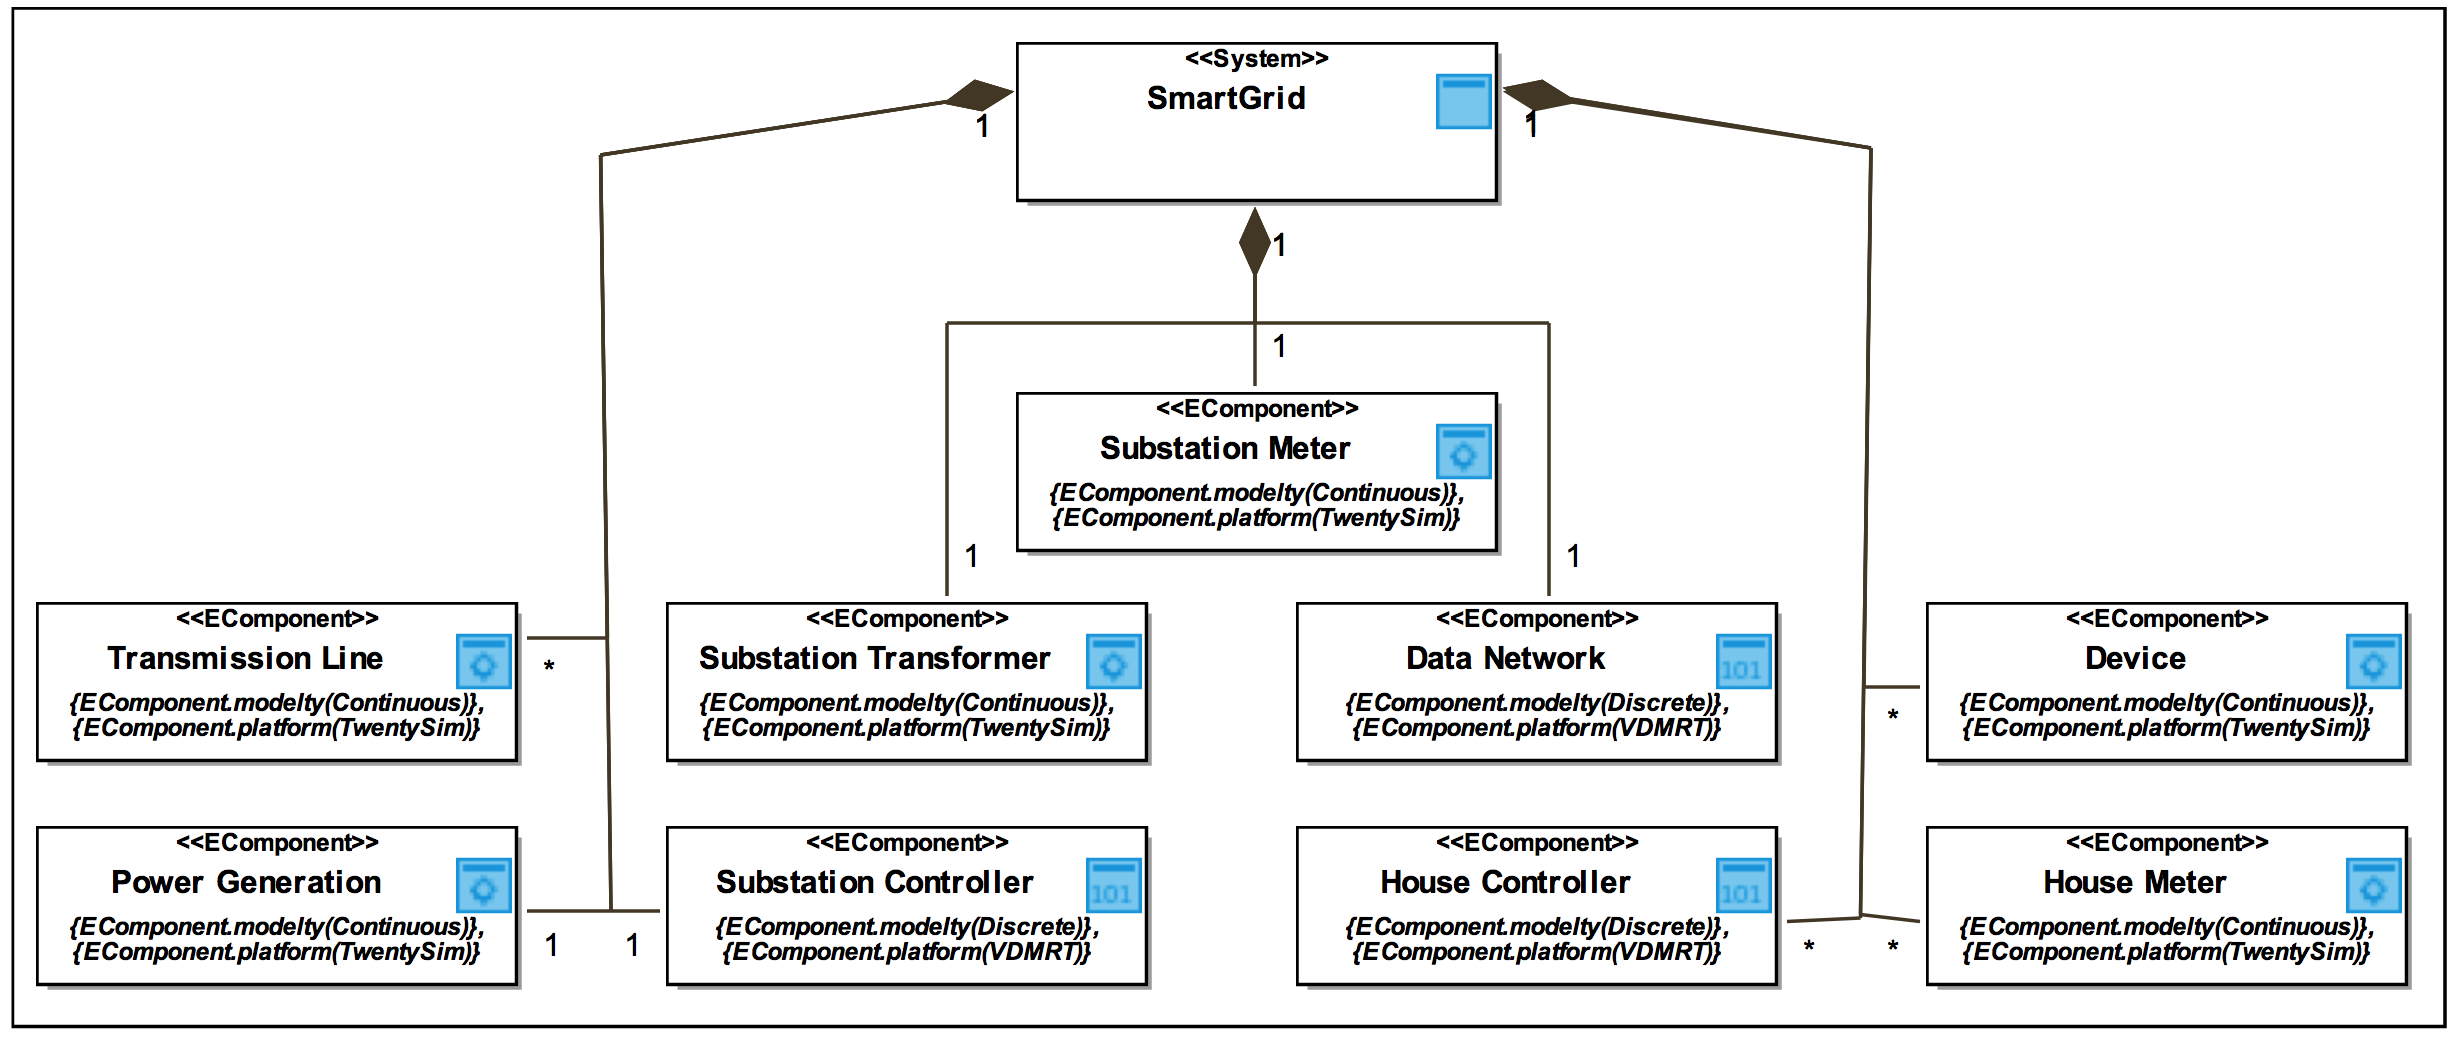
\includegraphics[width=0.9\textwidth]{figures/ASD_mm}
\caption{Architecture Structure Diagram for multi-model of Smart Grid}
\label{fig:asd_mm}
\end{figure}

The connections between the components are defined in the Connections Diagram (CD) in Figure~\ref{fig:cd_mm}. The interface between subsystems is defined as the interaction points between cyber and physical components (FMUs).

\begin{figure}
\centering
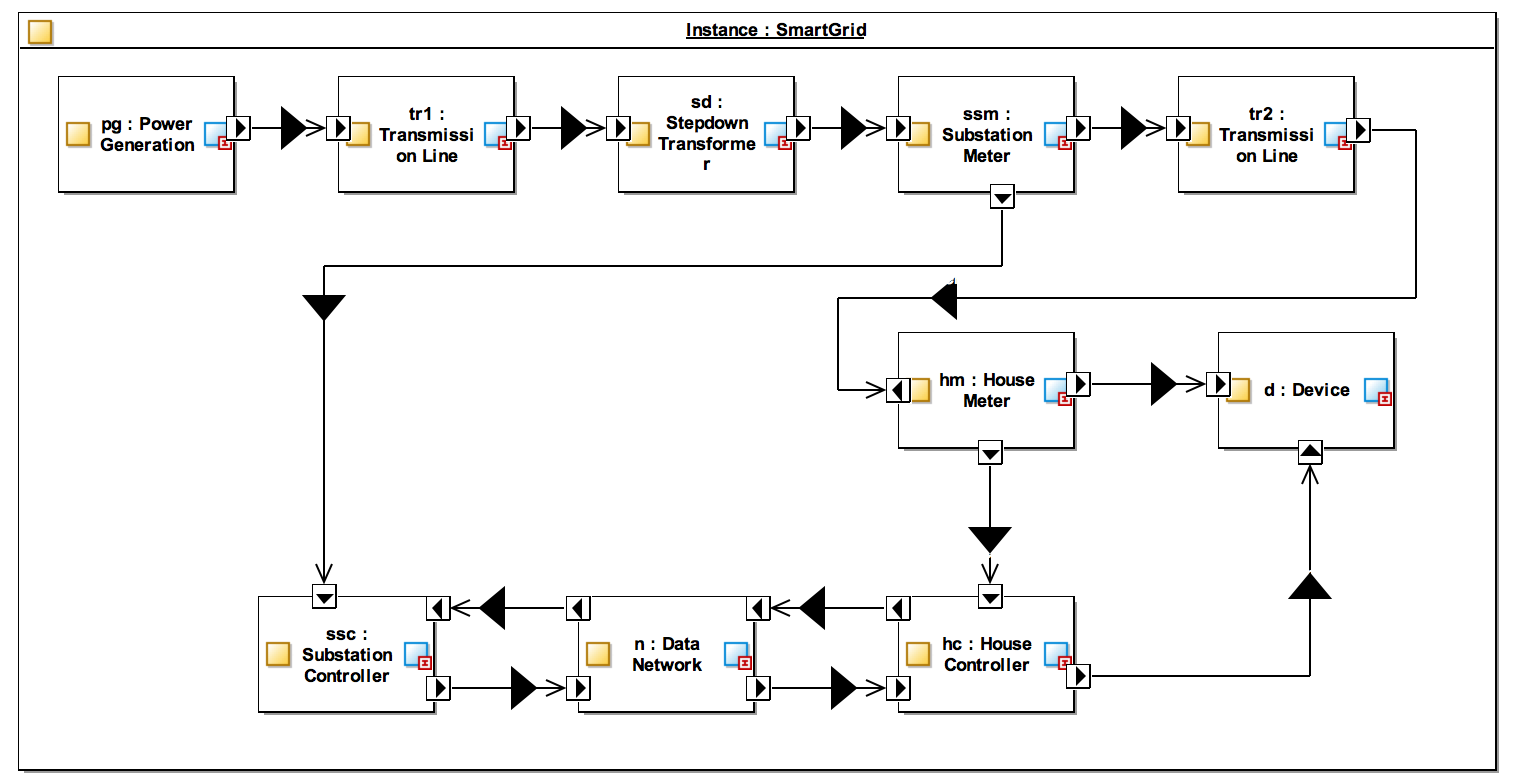
\includegraphics[width=1\textwidth]{figures/CD_mm}
\caption{Connections Diagram for multi-model of Smart Grid}
\label{fig:cd_mm}
\end{figure}

\subsubsection*{Discussion}

Contrasting the architectures shown in the initial model (Figures~\ref{fig:bdd} and~\ref{fig:ibd}) to that in the multi-model (Figures~\ref{fig:asd_mm} and~\ref{fig:cd_mm}), whilst the same base components are present in both, some of the intuitive domain-specific structures are lost when moving to a multi-model. For example, it is now not clear where the \emph{substation} or \emph{house} elements are in the multi-model.

An important issue here is in the reason behind producing different architectural models. Using SysML diagrams in a \emph{holistic} approach, a CPS engineer describes the model using a structure natural to the application domain. As such, the \emph{reason} for modelling is not in the ultimate analysis to perform, but to define and understand the structure and behaviour of a system. In contrast, the \emph{design} approach is necessary to configure INTO-CPS multi-models from SysML.

Figure~\ref{fig:sysml_mm} presents an overview of the relationships between the different types of models. The figure shows that the `real' system may be modelled in different forms: the holistic and design architectures and the multi-model.

\begin{figure}
\centering
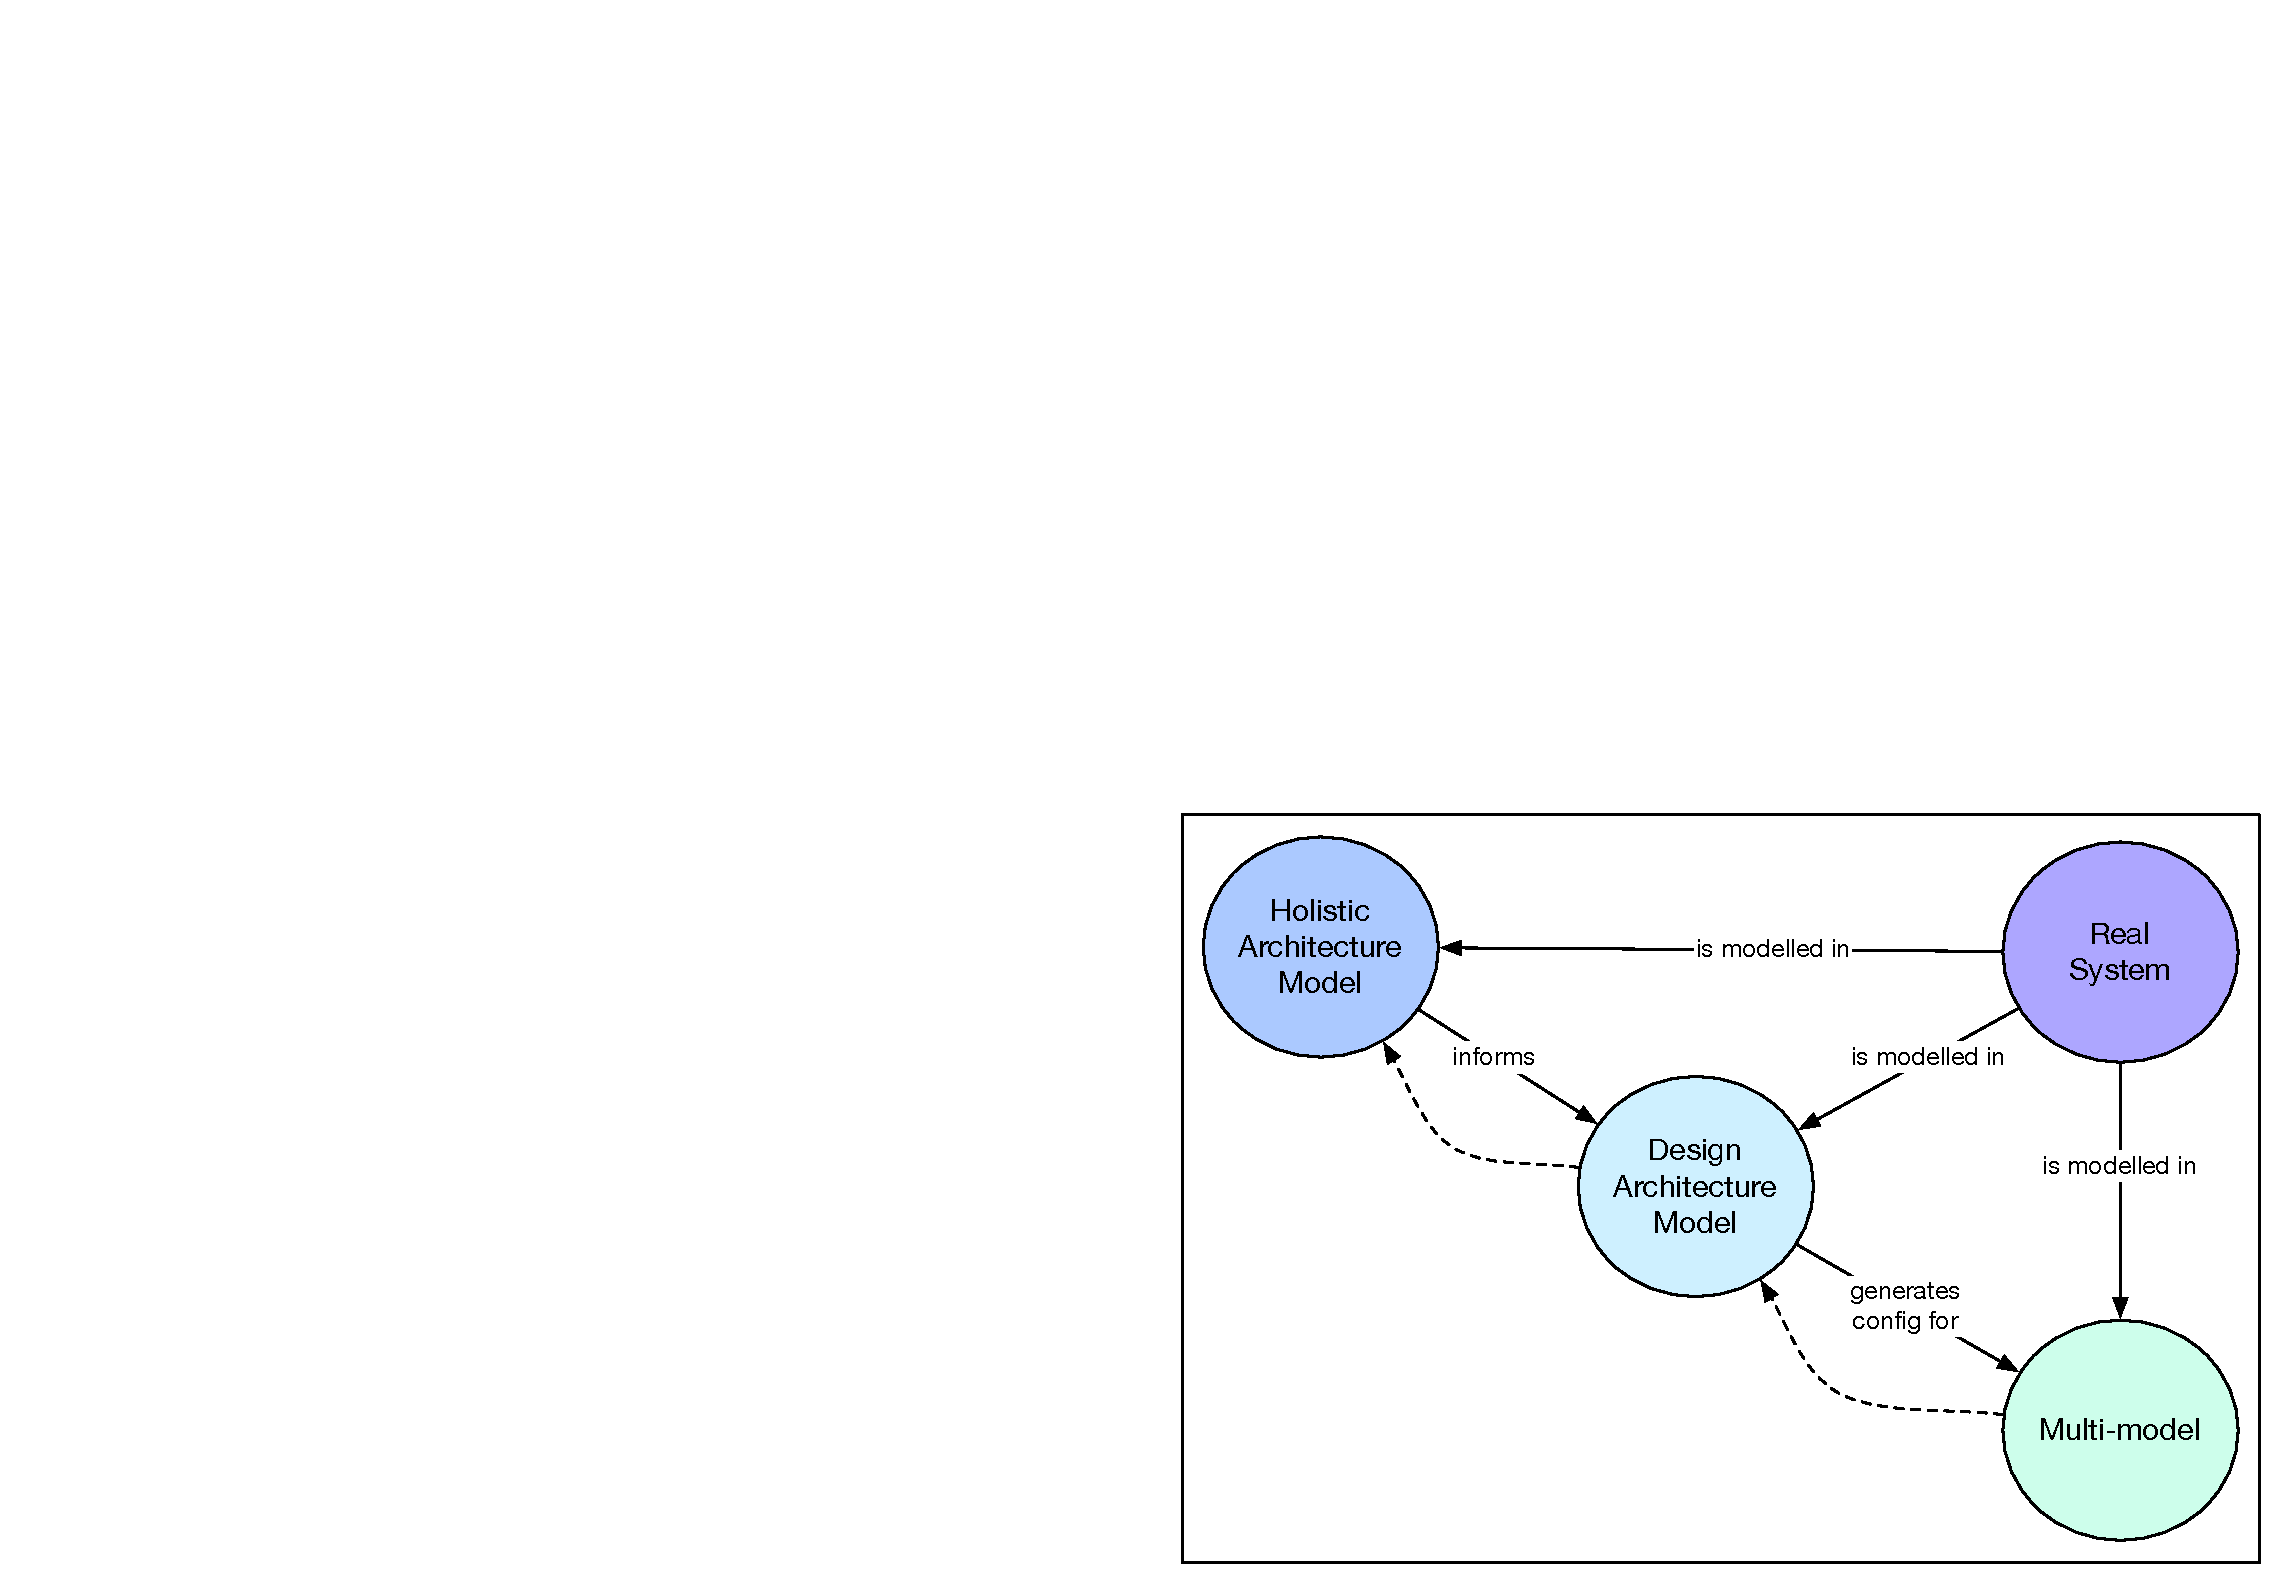
\includegraphics[width=0.7\textwidth]{figures/sysml_for_mm}
\caption{Relating holistic and design architectures}
\label{fig:sysml_mm}
\end{figure}

As illustrated in the figure, one approach can inform another. In some cases this may be a natural process; for example in the Smart Grid\ example, isolating each of the lowest level components in Figure~\ref{fig:bdd} to be individual FMUs in a multi-model is an evolution which will likely result in a feasible model. By creating a domain-specific holistic architecture first, then transforming these models into a design architecture for multi-modelling, design teams will likely gain the most benefit.


\section{Representing Non-Design Elements in SysML}
\label{sec:sysml:non-design}

Using the INTO-CPS tool chain, we generate co-simulation configurations using an architectural model defined with the INTO-SysML profile. This model defines the structure of a system in terms of the composition of its components and their connections. There are however circumstances where elements in the multi-model are not part of the design of the final system, for example where an FMU is used purely for visualisation. This FMU must be connected to the system components, however is not itself a system component. This is also true when considering the environment of the system.

Here we present a small example of the use of these extensions, using a simple robot example (based on the line-following robot pilot study, see Deliverable D3.6~\cite{INTOCPSD3.6}) to illustrate the use of \texttt{<<CComponent>>}s and the \emph{kind} of components (\emph{cyber}, \emph{physical}, \emph{environment}, \emph{visualisation}) described in Section~\ref{sec:sysml:intocps:asd} above.

The architecture structure diagram in Figure~\ref{fig:example_asd} shows: a \emph{System\_Env} block, an \texttt{<<EComponent>>} defined as an \texttt{Environment} FMU; a \emph{3D\_View} block an \texttt{<<EComponent>>}, defined as an \texttt{Visualisation} FMU; and an \emph{Example\_Robot} block, an \texttt{<<EComponent>>} defined as an \texttt{composition} of two FMUs.

\begin{figure}
\centering
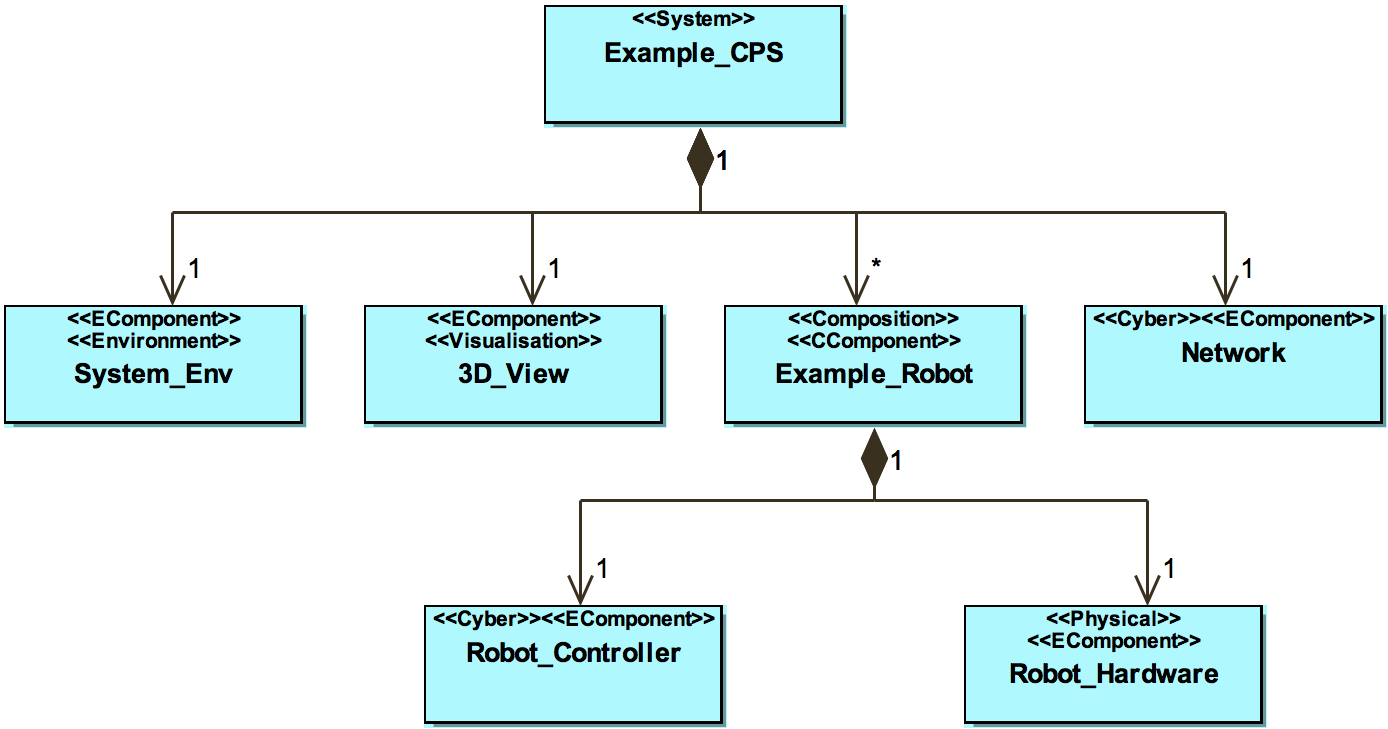
\includegraphics[width=0.8\textwidth]{figures/E_Blocks_ext_asd}
\caption{Example Architecture Structure Diagram of robot system}
\label{fig:example_asd}
\end{figure}

The example has two connection diagrams. The first is shown in Figure~\ref{fig:example_cd}, it contains only those connections with respect to the system and its constituent components . This diagram shows a block instance \emph{cps1} containing the environment (\emph{e}) and the example robot (\emph{r}) which  contains two the controller and hardware components.

The second is shown in Figure~\ref{fig:example_cd2}, it depicts the use of the block instance \emph{3D} of type \emph{3D\_View}. In this diagram, we show additional ports of the original block instances to output internal model details and connect these to the \emph{3D} instance. The diagram includes the system connectors as shown in Figure~\ref{fig:example_cd}.

\begin{figure}
\centering
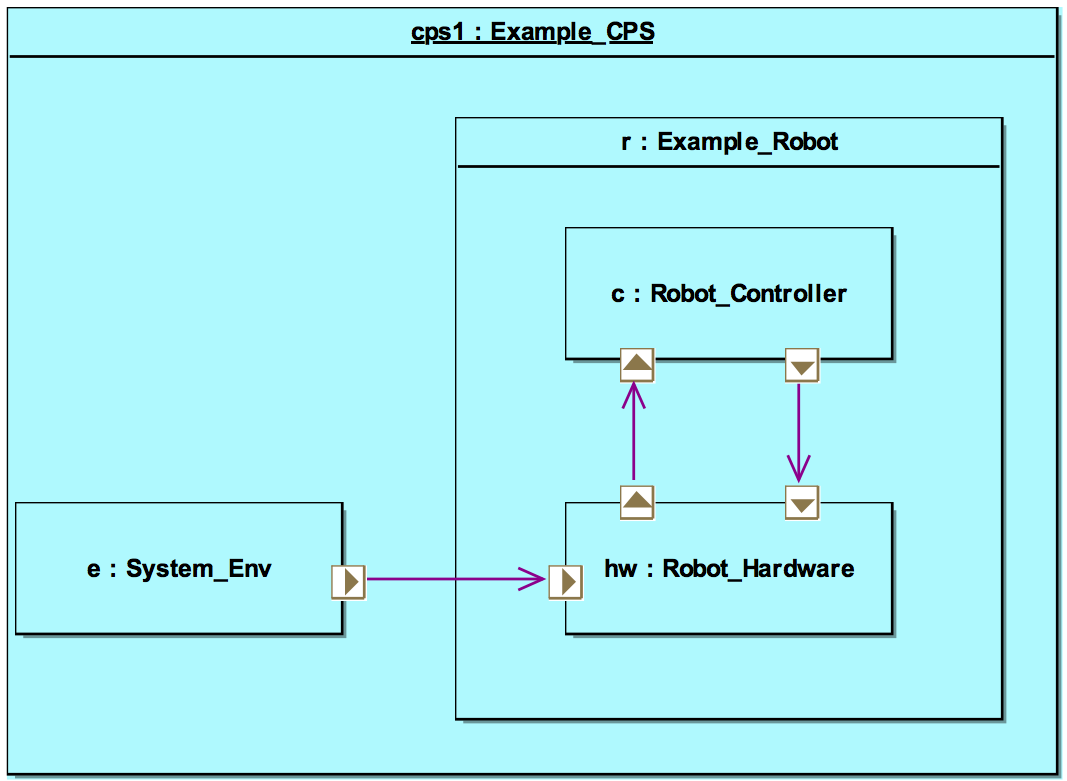
\includegraphics[width=0.6\textwidth]{figures/E_Blocks_ext_cd}
\caption{Connections Diagram for robot showing only system and environment connectors}
\label{fig:example_cd}
\end{figure}

\begin{figure}
\centering
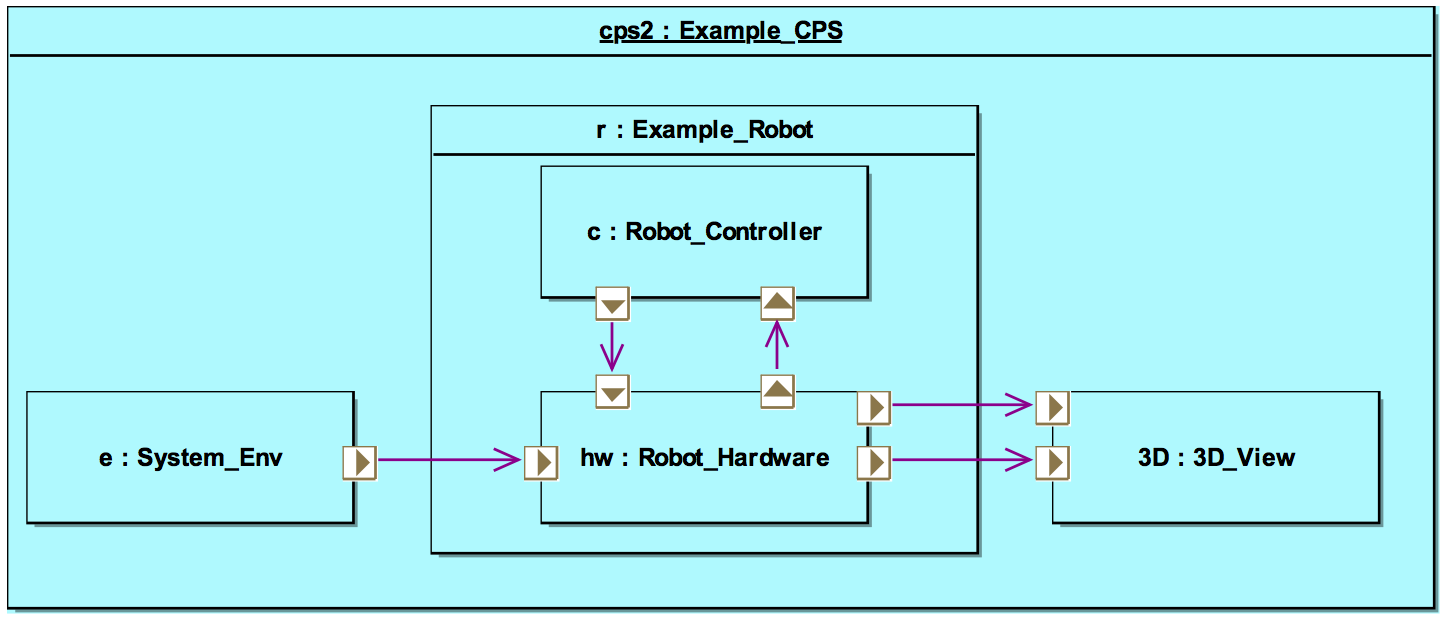
\includegraphics[width=0.9\textwidth]{figures/E_Blocks_ext_cd2}
\caption{Connections Diagram for the robot system showing the system \textit{and} visualisation components}
\label{fig:example_cd2}
\end{figure}










%
% MOVED TO D4.2c
%

%\section{Metamodel and Profile Extensions}
%
%As such, we have extended the INTO-CPS SysML metamodel and profile to allow a multi-model to include an FMU for visualisation and the environment, the addition of the CComponents type and an extension for FlowPorts to support minimum and maximum values in later versions of the SysML-FMI translation.
%
%In this document we present the extensions to INTO-SysML first in metamodel fragments (Figure~\ref{fig:mm-extensions}) and then as SysML profile diagrams (Figure~\ref{fig:profile-extensions}), as presented in~\cite{INTOCPSD2.1a}. In Figure~\ref{fig:fblocks_ext}, we extend the F\_Blocks metamodel fragment to include CComponents, additional ComponentKind enumerations and the repositioning of Flowport ownership -- changes are shown in red. The diagram shows that a \texttt{CComponent} is a subtype of \texttt{Component}, and contains no additional attributes. To support modelling of non-CPS components, three extra \texttt{ComponentKind} enumerations are added: \texttt{environment}, \texttt{visualisation} and \texttt{composition}. Finally, where previously the \texttt{Block} stereotype was the owner of \texttt{FlowPorts}, we have adjusted that relationships so that neither \texttt{System} or \texttt{CComponent} instances can own \texttt{FlowPorts}.
%
%A minor update to the \texttt{FlowPort} definition is shown in Figure~\ref{fig:port_ext}. The extension is to allow minimum and maximum values for flowports to be defined. The \texttt{min} and \texttt{max} attributes are of type PType -- the primitive types of INTO-SysML.
%
%\begin{figure}[htbp]
%\begin{center}
%\subfigure[Extension to F\_Blocks fragment]
%{
%	\includegraphics[width=0.5\textwidth]{figures/MM_Blocks}
%	\label{fig:fblocks_ext}
%}
%\subfigure[Extension to F\_Props fragment]
%{
%	\includegraphics[width=0.4\textwidth]{figures/MM_Ports}
%	\label{fig:port_ext}
%}
%\caption{Extended Metamodel fragments of INTO-SysML -- extensions are highlighted with a red dotted line.}
%\label{fig:mm-extensions}
%\end{center}
%\end{figure}
%
%The next collection of figures present the extensions to the INTO-SysML profile, which implement the above metamodel extensions. Figure~\ref{fig:profile-blocks-comp} realises the composition aspect of F\_Blocks metamodel fragment in Figure~\ref{fig:fblocks_ext}. Two extensions are defined: firstly a specialisation of the \texttt{Component} stereotype, \texttt{CComponent} is defined; and secondly the three additional options for the \texttt{ComponentKind} enumeration are defined.
%
%Figure~\ref{fig:profile-blocks-conn} presents a realisation of the F\_Props metamodel in Figure~\ref{fig:port_ext}, and the reorganisation of FlowPort ownership from the F\_Blocks metamodel fragment in Figure~\ref{fig:fblocks_ext}. Two main changes are defined. The first, adds two new tags to the \texttt{FlowPort} stereotype -- \texttt{min} and \texttt{max}. The second change is the adjustment of flowport ownership. In the original profile a \texttt{Block} may own \texttt{FlowPorts}, we have changed this to reflect the metamodel and so the \texttt{EComponent} and \texttt{POComponents}\footnote{A PComponent, as defined in Deliverable D2.1a~\cite{INTOCPSD21a} is an \emph{Part-of Component}, corresponding to an internal element of an encapsulated component.} are the only to \texttt{Block}  specialisations that may own the ports.
%
%\begin{figure}[htbp]
%\begin{center}
%\subfigure[Blocks compositon]
%{
%	\includegraphics[width=0.5\textwidth]{figures/Profile_Blocks1}
%	\label{fig:profile-blocks-comp}
%}
%\subfigure[Blocks connections]
%{
%	\includegraphics[width=0.9\textwidth]{figures/Profile_Blocks2}
%	\label{fig:profile-blocks-conn}
%}
%\caption{Extension to INTO-CPS SysML Profile}
%\label{fig:profile-extensions}
%\end{center}
%\end{figure}
%
%In the next section we provide an example of the use of these extensions.

%\section{Illustrative Example}


\chapter{Initial Multi-Modelling using VDM}
\label{sec:initial}

In this section we provide guidance on producing initial multi-models from architectural descriptions produced using the INTO-CPS SysML profile. We focus on using discrete-event (DE) models to produce initial, abstract FMUs that allow integration testing through co-simulation before detailed modelling work is complete. This is called a ``DE-first'' approach~\cite{Fitzgerald&13b,Fitzgerald&13a}. We describe the use of VDM and the Overture tool, with FMI export plug-in installed, for this approach. The principles outlined in this section can be applied in other modelling tools. This approach can work with or without the SysML profile.

%In future, these guidelines will be expanded to include how and when to continuous-time (CT) formalisms in initial modelling.

%\section{Context}
\section{The DE-first Approach}

\begin{figure}[p]
\centering
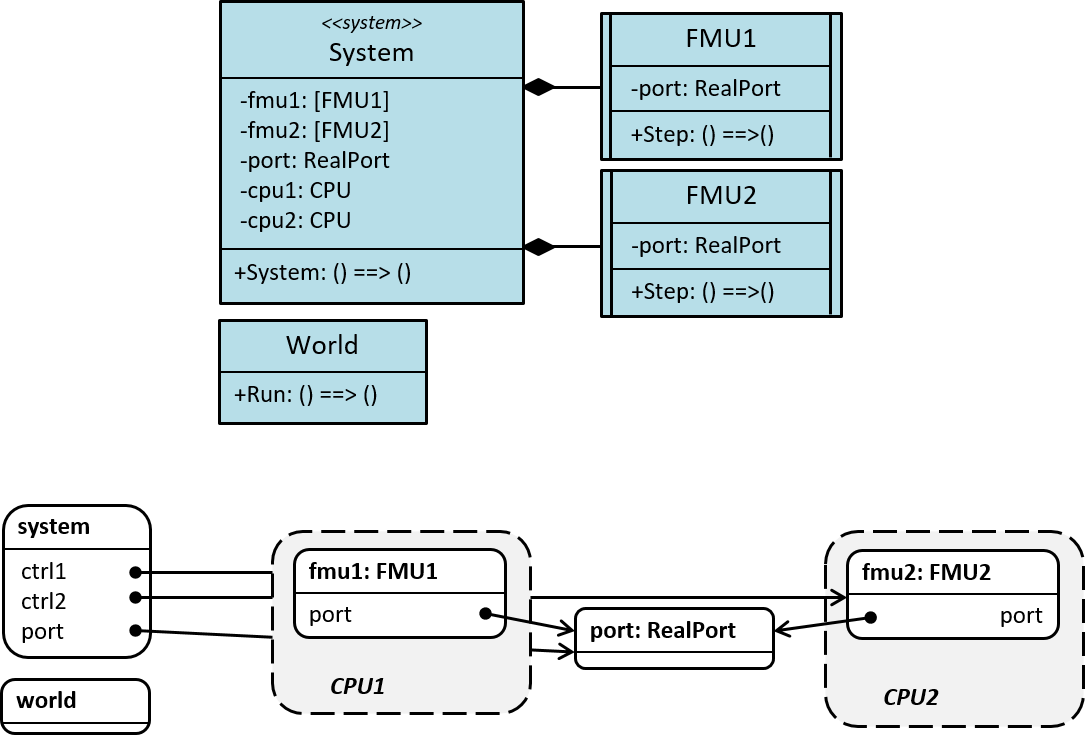
\includegraphics[scale=0.47]{figures/defirst_class}
\caption{Class diagram showing two simplified FMU classes created within a single VDM-RT project, and an object diagram showing them being instantiated as a test.}
\label{fig:defist_class}
\end{figure}

\begin{figure}[p]
\centering
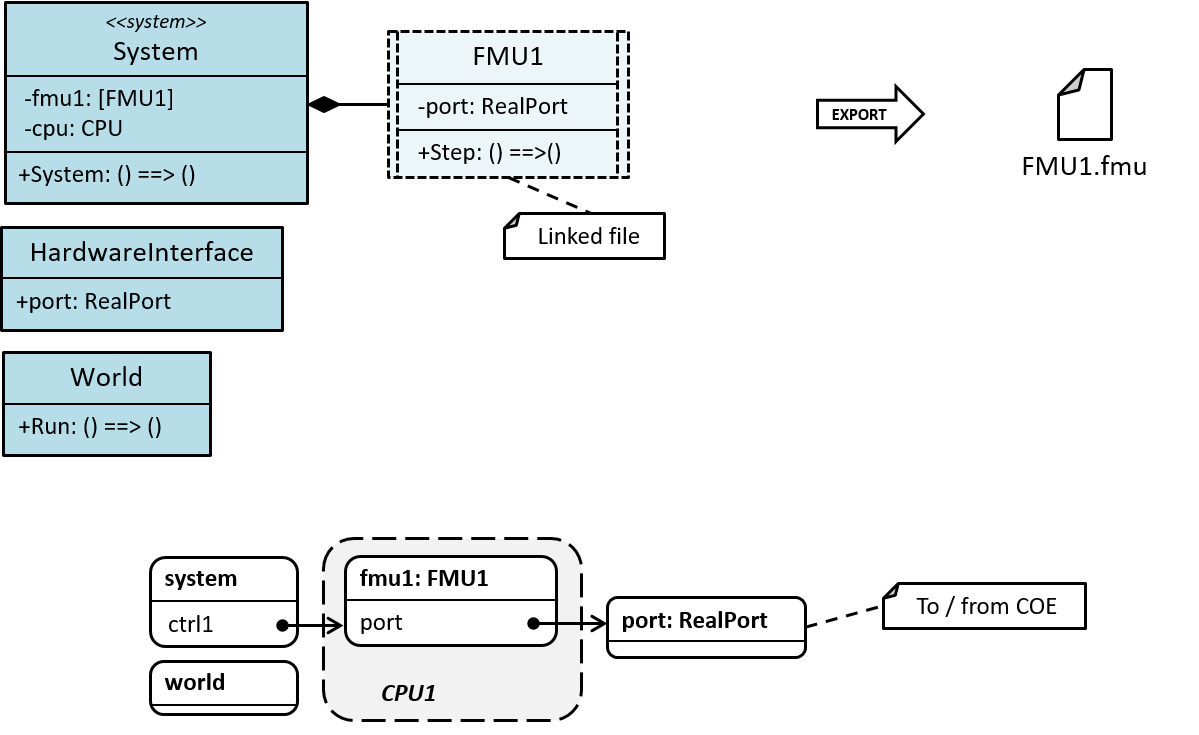
\includegraphics[scale=0.47]{figures/defirst_fmu1}
\caption{Class and object diagrams showing a linked class within its own project for FMU creation.}
%\begin{center}
%\subfigure[Structure of the FMU1 project]
%{
%	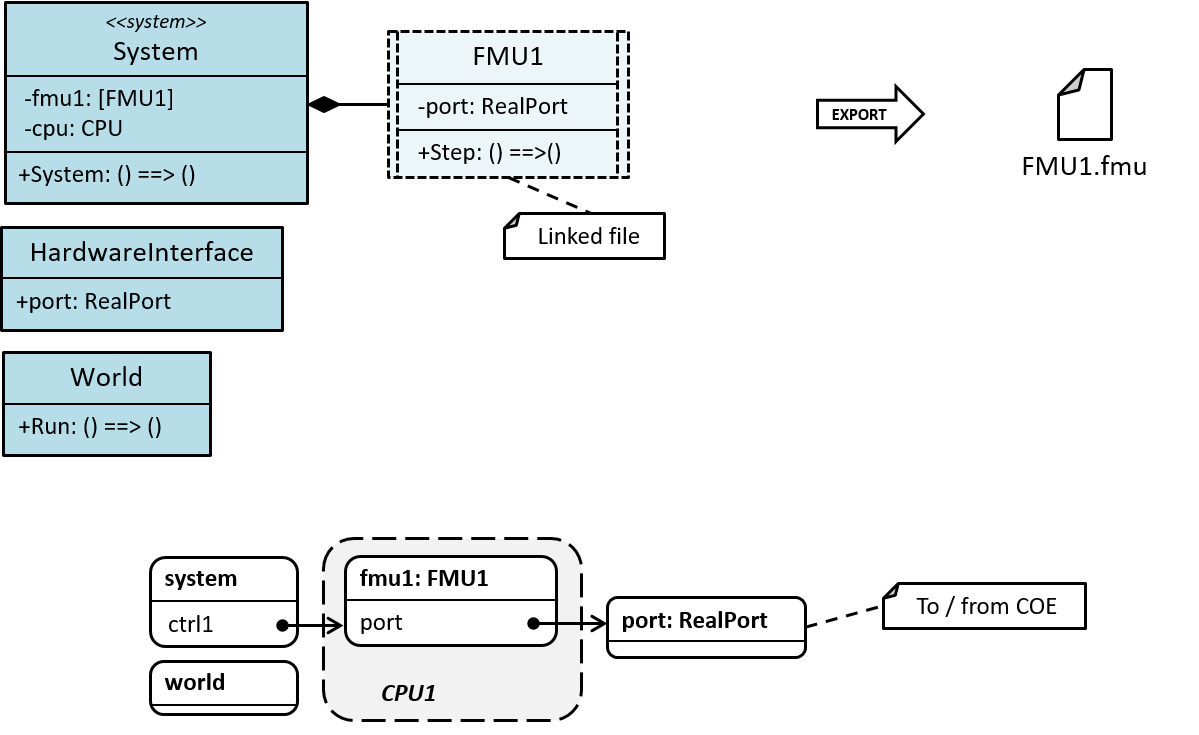
\includegraphics[scale=0.4]{figures/defirst_fmu1}
%	\label{fig:snd_rec}
%}
%\subfigure[Structure of the FMU2 project]
%{
%	\includegraphics[scale=0.4]{figures/defirst_fmu2}
%	\label{fig:snd_ether_rec}
%}
%\caption{Class diagrams showing the FMU classes being included (through file linking) in their own projects ready for export to FMU}
\label{fig:defirst_fmus}
\end{figure}

After carrying out requirements engineering (RE), as described in Chapter~\ref{sec:reqeng}, and design architectural modelling in SysML, as described in Chapter~\ref{sec:sysml}, the engineering team should have the following artifacts available:

\begin{itemize}[noitemsep]
\item One or more Architecture Structure Diagrams (ASDs) defining the composition of\\ \texttt{<<EComponent>>}s (to be realised as \texttt{<<Cyber>>} or \texttt{<<Physical>>} FMUs) that will form the multi-model.
\item Model descriptions exported for each \texttt{<<EComponent>>}.
\item One or more Connections Diagrams (CDs) that will be used to configure a multi-model.
\end{itemize}

The next step is to generate a multi-model configuration in the INTO-CPS Application and populate it with FMUs, then run a first co-simulation. This however requires the source models for each FMU to be ready. If they already exist this is easy, however they may not exist if this is a new design. In order to generate these models, the model descriptions for each \texttt{<<EComponent>>} can be passed to relevant engineering teams to build the models, then FMUs can be passed back to be integrated.

It can be useful however to create and test simple, abstract FMUs first (or in parallel), then replace these with higher-fidelity FMUs as the models become available. This allows the composition of the multi-model to be checked early, and these simple FMUs can be reused for regression testing. This approach also mitigates the problem of modelling teams working at different rates.

Where these simple FMUs are built within the DE formalism (such as VDM), this is called a \emph{DE-first} approach. This approach is particularly appropriate where complex DE control behaviours ---such as supervisory control or modal behaviours--- are identified as a priority or where the experience of the modelling team is primarily in the DE domain~\cite{Fitzgerald&14c}.

Guidance on how to produce DE approximations for use in multi-modelling, and in particular approximations of CT behaviour, can be found in material describing the Crescendo baseline technology~\cite{Fitzgerald&13a}, which is also available via the Crescendo website\footnote{See \url{http://crescendotool.org/documentation/}}.

\section{DE-first within INTO-CPS}

Given an architectural structure diagram, connections diagram and model descriptions for each \texttt{<<EComponent>>}, the suggested approach is to begin by building a single VDM-RT project in Overture with the following elements:

\begin{itemize}[noitemsep]
\item A class for each \texttt{<<EComponent>>} representing an FMU. Each class should define port-type instance variables (i.e. of type \texttt{IntPort}, \texttt{RealPort}, \texttt{BoolPort}, or \texttt{StringPort}) corresponding to the model description and a constructor to take these ports as parameters. Each FMU class should also define a thread that calls a \texttt{Step} operation, which should implement some basic, abstract behaviour for the FMU.
\item A \texttt{system} class that instantiates port and FMU objects based on the connections diagram. Ports should be passed to constructor of each FMU object. Each FMU object should be deployed on its own CPU.
\item A \texttt{World} class that starts the thread of each FMU objects.
\end{itemize}

Class and object diagrams giving an example of the above is shown in Figure~\ref{fig:defist_class}. In this example, there are two \texttt{<<EComponent>>}s (called \emph{FMU1} and \emph{FMU2}) joined by a single connection of type real. Such a model can be simulated within Overture to test the behaviour of the FMUs. This approach can be combined with the guidance in Chapter~\ref{sec:networks} to analyse more complicated networked behaviour. Once the behaviour of the FMU classes has been tested, actual FMUs can be produced and integrated into a first multi-model by following the guidance below.

\section{FMU Creation}

The steps outlined below assume a knowledge of FMU export in Overture, which can be found in the User Manual, Deliverable D4.3a~\cite{INTOCPSD4.3a}, in Section 5.1. To generate FMUs, a project must be created for each \texttt{<<EComponent>>} with:

\begin{itemize}[noitemsep]
\item One of the FMU classes from the main project.
\item A \texttt{HardwareInterface} class that defines the ports and annotations required by the Overture FMU export plug-in, reflecting those defined in the model description.
\item A \texttt{system} class that instantiates the FMU class and passes the port objects from the \texttt{HardwareInterface} class to its constructor.
\item A \texttt{World} class that starts the thread of the FMU class.
\end{itemize}

The above structure is shown in Figure~\ref{fig:defirst_fmus}. A skeleton project with a correctly annotated \texttt{HardwareInterface} class can be generated using the model description import feature of the Overture FMU plug-in. The FMU classes can be linked into the projects (rather than hard copies being made) from the main project, so that any changes made are reflected in both the main project and the individual FMU projects. These links can be created by using the \emph{Advanced} section of the \emph{New \textgreater\ Empty VDM-RT File} dialogue, using the \texttt{PROJECT-1-PARENT\_LOC} variable to refer to the workspace directory on the file system (as shown in Figure~\ref{fig:defirst_link}). Note that if the FMU classes need to share type definitions, these can be created in a class called \texttt{Types} in the main project, then this class can be linked into each of the FMU projects in the same way.

From these individual project, FMUs can be exported and co-simulated within the INTO-CPS tool. These FMUs can then be replaced as higher-fidelity versions become available, however they can be retained and used for regression and integration testing by using different multi-model configurations for each combination.

\begin{figure}
\centering
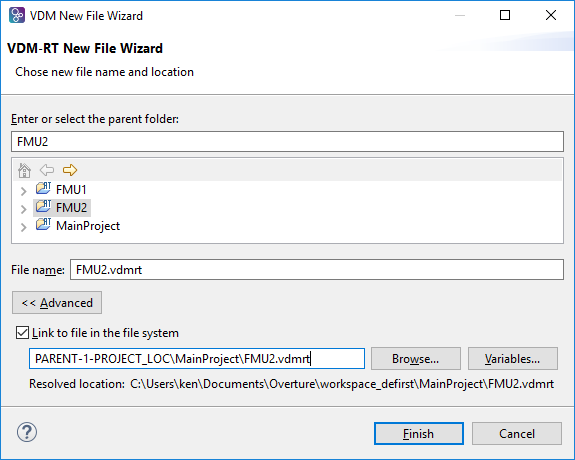
\includegraphics[scale=0.8]{figures/defirst_link}
\caption{Linking files in the \emph{New \textgreater\ Empty VDM-RT File} dialogue.}
\label{fig:defirst_link}
\end{figure}

\begin{figure}
\centering
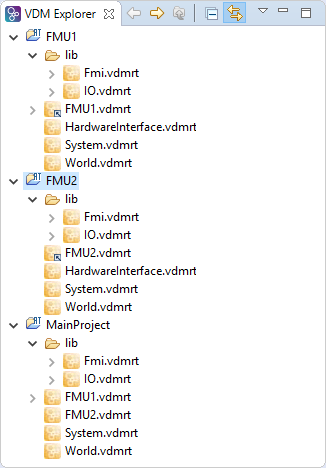
\includegraphics[scale=0.8]{figures/defirst_workspace}
\caption{Project structure of an Overture workspace showing a main project and two projects used for generating FMUs from linked class files.}
\label{fig:defirst_workspace}
\end{figure}


%\begin{figure}
%\centering
%\includegraphics[scale=0.4]{figures/defirst_object}
%\caption{Object showing two controllers being simulated within a main project, and being co-simulated in their own FMUs}
%\label{fig:defist_object}
%\end{figure}


\chapter{Modelling Networks with VDM in Multi-models}
\label{sec:networks}

In this section, we address the problem of modelling networked controllers in multi-models, presenting a solution using VDM. When modelling and designing distributed controllers, it is necessary to model communications between controllers as well. While controller FMUs can be connected directly to each other through for co-simulation, this quickly becomes unwieldy due to the number of connections increasing exponentially. For example, consider the case of five controllers depicted in Figure~\ref{fig:bigraph}. In order to connect each controller together, 20 connections are needed (i.e.\ for a complete bidirected graph). Even with automatic generation of multi-model configurations, this is in general not a feasible solution.

\begin{figure}[hb]
\centering
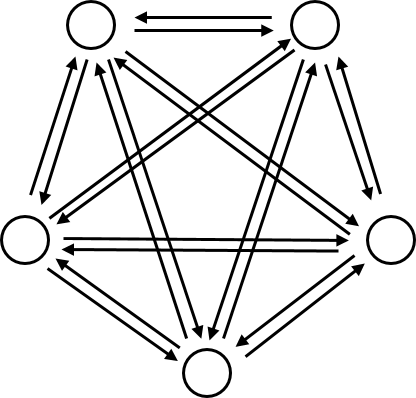
\includegraphics[scale=0.4]{figures/bigraph}
\caption{Topology of five controllers connected to each other}
\label{fig:bigraph}
\end{figure}

We suggest employing a pattern described initially as part of the Crescendo technology~\cite{Fitzgerald&14c}, in which a representation of an abstract communications medium called the `ether' is introduced. In the INTO-CPS setting, the ether is an FMU that is connected to each controller that handles message-passing between them. This reduces the number of connections needed, particularly for large numbers of controllers such as swarms. For five controllers, only 10 connections are needed, as shown in Figure~\ref{fig:bigraph2}.

\begin{figure}[hb]
\centering
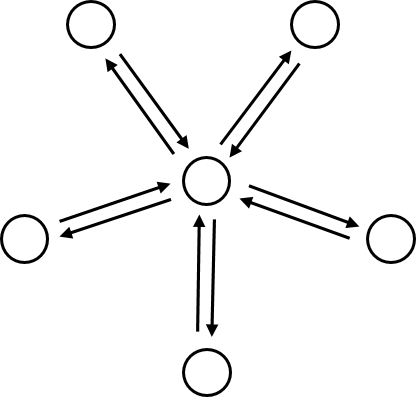
\includegraphics[scale=0.4]{figures/bigraph2}
\caption{Topology of five controllers connected via a shared medium}
\label{fig:bigraph2}
\end{figure}

In the remainder of this section, we describe how to pass messages between VDM FMUs using string types, how the ether class works, some of the consequences of using the ether pattern, and finally some extensions for providing quality of service (QoS) guarantees. %A class listing for a reference implementation of the \texttt{Ether} class is given in Appendix~\ref{app:ether}.
An example multi-model, called \emph{Case Study: Ether}, is available from the INTO-CPS Application. It is also described in the Examples Compendium, Deliverable D3.6~\cite{INTOCPSD3.6}.

\section{Representing VDM Values as Strings}

Connections between FMUs are typically numerical or Boolean types. This works well for modelling of discrete-time (DT) controllers and continuous-time (CT) physical models, however one of the advantages of VDM is the ability to represent more complex data types that better fit the abstractions of supervisory control. Therefore, in a multi-modelling setting, it is advantageous if VDM controllers can communicate with each other using data types that are not part of the FMI specification.

This can be achieved by passing strings between VDM FMUs (which are now supported by the Overture FMU export plug-in) and the \texttt{VDMUtil} standard library included in Overture, which can convert VDM types to their string representations and back again.

The \texttt{VDMUtil} library provides a (polymorphic) function called \texttt{val2seq\_of\_char}, that converts a VDM type to a string. It is necessary to tell the function what type to expect as a parameter in square brackets. For example, in the following listing, a 2-tuple is passed to the function, which will produce the output \texttt{"mk\_(2.4, 1.5)"}:

\begin{vdm}
VDMUtil`val2seq_of_char[real*real](mk_(2.4, 1.5))
\end{vdm}

The above can be used when sending messages as strings. In the model receiving message, the inverse function \texttt{seq\_of\_char2val} can be used. This function returns two values, a Boolean value indicating if the conversion was successful, and the value that was received:

\begin{vdm}
let mk_(b,v) = VDMUtil`val2seq_of_char[real*real](msg) in
  if b then ...
\end{vdm}

In the first few steps of co-simulation, empty or invalid strings are often passed as values, so it is necessary to check if the conversion was successful (as in the above listing) before using the value.

Note that currently (as of Overture 2.4.0), the \texttt{VDMUtil} library is called in the default scope, meaning that it does not know about custom types defined in the model. Therefore, it is recommended to pack values in a tuple (as in the above example) for message passing, then convert to and from any custom types in the sending and receiving models.

\section{Using the Ether FMU}

\begin{figure}
\centering
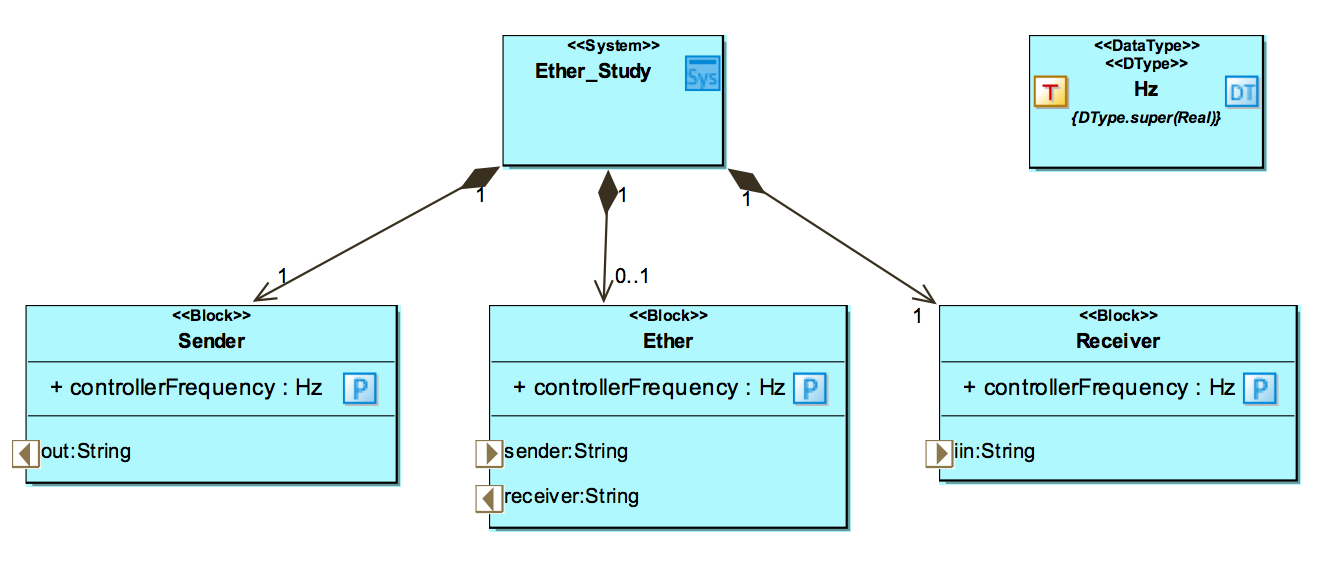
\includegraphics[scale=0.3]{figures/ether_asd}
\caption{\emph{Case Study: Ether} example}
\label{fig:ether_asd}
\end{figure}

By encoding VDM values as strings, it is possible to define a simple broadcast ether that receives message strings on its input channel(s) and sends them to its output channel(s). As a concrete example, we consider the \emph{Case Study: Ether} (see Deliverable D3.5~\cite{INTOCPSD3.5}), which contains a \texttt{Sender}, a \texttt{Receiver} and an \texttt{Ether}, as depicted in Figure~\ref{fig:ether_asd}. In this example, the three FMUs have the following roles:

\begin{description}[noitemsep]
  \item[Sender] Generates random 3-tuple messages of type \texttt{real * real * real}, encodes them as strings using the \texttt{VDMUtil} library and puts them on its output port.
  \item[Receiver] Receives strings on its input port and tries to convert them to single messages of type \texttt{real * real * real} or to a sequence of messages of type of type \texttt{seq of (real * real * real)}.
  \item[Ether] Has an input port and output port, each assigned a unique identifier, i.e. as a \texttt{map Id to StringPort}. It also has a mapping of input to output ports as a set of pairs: \texttt{set of (Id * Id)}. It has a list that holds messages for each output destination, because multiple messages might arrive for one destination. It gathers messages from each input and passes them to the outputs defined in the above mapping.
\end{description}

In this simple example, the sender and receiver are asymmetrical, but in more complicated examples controllers can be both senders and receivers by implementing both of the behaviours described above.

The \emph{Case Study: Ether} example contains two multi-models that allow the sender and receiver to be connected directly (connection diagram shown in Figure~\ref{fig:snd_rec}), or to be connected via the ether (connection diagram shown in Figure~\ref{fig:snd_ether_rec}). The description in the Examples Compendium, Deliverable D3.5~\cite{INTOCPSD3.5}, explains how to run the two different multi-models. This approach shows that the use of string ports and the \texttt{VDMUtil} library can be useful even without the ether for message passing between controllers in simple topologies.

For the sender, this connection is transparent, it does not care whether it is connected to the ether or not. For the receiver, in the direct connection it will receive single messages, whereas when receiving from the ether it will receive a list of messages (even for a single value). So the receiver is able to deduce when it is directly connected or connected via the ether. %Later in this section, when we describe quality of service, it is n



\begin{figure}
\begin{center}
\subfigure[Connection diagram of the \emph{Direct} multi-model in the \emph{Case Study: Ether} example]
{
	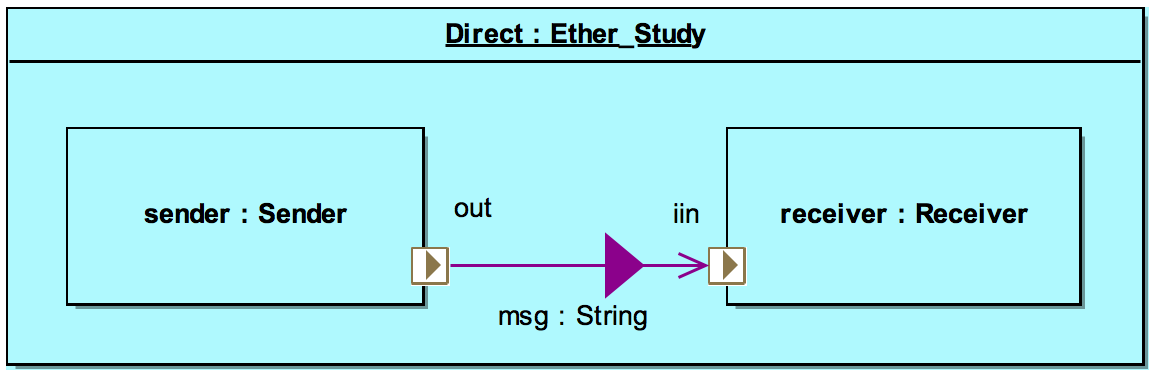
\includegraphics[scale=0.2]{figures/ether_cd_direct}
	\label{fig:snd_rec}
}
\subfigure[Connection diagram of the \emph{Ether} multi-model in the \emph{Case Study: Ether} example]
{
	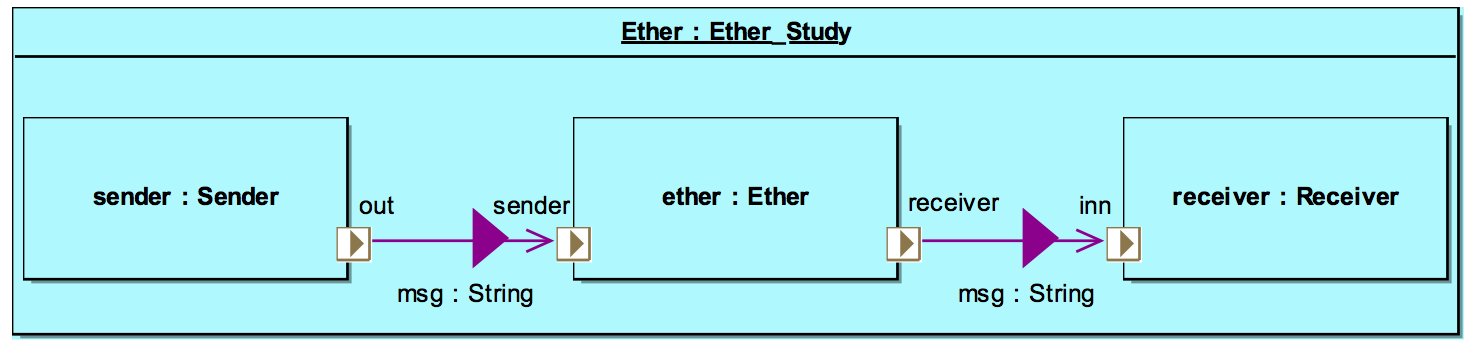
\includegraphics[scale=0.25]{figures/ether_cd_ether}
	\label{fig:snd_ether_rec}
}
\caption{Alternative multi-models in the \emph{Case Study: Ether} example}
\label{fig:cds}
\end{center}
\end{figure}

The ether defined in this example is intended to be generic enough that it can be used in other case studies that need a simple broadcast ether without guarantees of delivery. To use it, you can:

\begin{enumerate}[noitemsep]
\item Import the \emph{Ether} model from the \emph{case-study\_ether/Models} directory into Overture;
\item Update the \texttt{HardwareInterface}\footnote{A class that provides annotated definitions of the ports for a VDM FMU.} class to provide input and/or output ports for all controllers that will be connected to the ether.
\item Update the \texttt{System} class to assign identifiers to all input and output ports; and
\item Update the set of identifier pairs that define connections.
\end{enumerate}

\section{Consequences of Using the Ether}

The ether as presented above %, and listed in Appendix~\ref{app:ether},
is fairly basic. In each update cycle, it passes values from its input variables to their respective output variables. This essentially replicates the shared variable style of direct FMU-FMU connections, which means that the relative update speeds of the FMUs may lead to the following:

\begin{description}[noitemsep]
  \item[Values may be delayed] The introduction of an intermediate FMU means that an extra update cycle is required to pass values from sender to ether and ether to receiver. This may delay messages unless the ether updates at least twice as fast as the receiver.
  \item[Values may not be read] If a value is not read by the receiver before it is changed, then that value is lost.
  \item[Values may be read more than once] If a value is not changed by the sender before the receiver updates, then the value is read twice. In the simple ether, the receiver cannot distinguish an old message from a new message with the same values.
\end{description}

In the Examples Compendium, Deliverable D3.5~\cite{INTOCPSD3.5}, the \emph{Case Study: Ether} example is described along with some suggested experiments to see the effects of the above examples by changing the controller frequency parameters of the sender, ether and receiver. In the final part of this section we outline ways to overcome such problems if it is necessary to guarantee that messages arrive and are read during a co-simulation.

\section{Modelling True Message Passing and Quality of Service}

The key to achieving a true message-passing is to overcome the problem of distinguishing old messages from new messages with the same values. This can be done by attaching a unique identifier to each message, which could be, for example, an identifier of the sender plus a message number:

\newpage
\begin{vdm}
instance variables

id: seq of char := "a";
seqn: nat1 := 1;

...

VDMUtil`val2seq_of_char[seq of char*real*real](
  mk_(id ^ [seqn], 2.4, 1.5));
seqn := seqn + 1
\end{vdm}

The advantage of assigning an identifier to each controller is that messages could also contain destination addresses, instead of the broadcast model presented above. In order to achieve these, some changes are needed to allow for acknowledging receipt of messages. Controllers should:

\begin{enumerate}[noitemsep]
\item Send a queue of messages on their output channel along with message identifiers of (recently received) messages;
\item Expect to receive a queue of messages along with message identifiers of successfully sent messages; and
\item Senders should remove messages from their output queue once their receipt has been acknowledged.
\end{enumerate}

The \texttt{Ether} class must be extended to:

\begin{enumerate}[noitemsep]
\item Inspect the message identifier (and destination if required) using \texttt{VDMUtil};
\item Pass message identifiers back to senders to acknowledge receipts; and
\item Listen for message identifiers from receivers to know when to remove messages from the queue.
\end{enumerate}

A dedicated channel for acknowledging messages could also be introduced, which would simplify the above. Therefore, each controller would have four connections to the ether: send and acknowledge, receive and acknowledge, as depicted in Figure~\ref{fig:ack}.

\begin{figure}
\centering
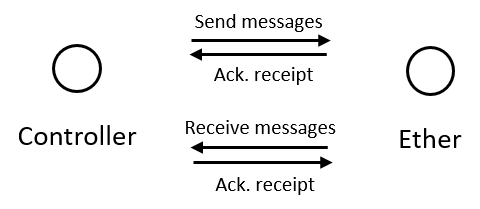
\includegraphics[scale=0.6]{figures/ack_channel}
\caption{Topology of controller to \emph{Ether} connection with dedicated channels for messages and acknowledgements}
\label{fig:ack}
\end{figure}

The advantages of guaranteed message delivery as described here are that realistic and faulty behaviour of the communication medium can be studied. An ether can be produced that provides poorer quality of service (delay, loss, repetition, reordering). These behaviours could be parameterised and explored using DSE (see Chapter~\ref{sec:dse}). By controlling for problems introduced by the nature of co-simulation, any reduction in performance of the multi-model can be attributed to the realistic behaviour introduced intentionally into the model of communications.


\chapter{Design Space Exploration}
\label{sec:dse}

In this section, we outline guidelines for  DSE over co-models of CPSs that: (a) support decision management by helping engineers to articulate clearly the parameters, objectives and metrics of a DSE analysis (Section~\ref{sec:dse-sysml}); and (b) enable the tuning of DSE methods for given domains and systems of interest (Section~\ref{sec:dse-algorithms}).
%
%
%\section{Experiment variables}
%
%\fbox{introduce parameters, architectures and scenarios and how they differ}
%
%

%
%\section{Ranking of designs}
%
%\fbox{methods for ranking and how they differ}
%


\section{Guidelines for Designing DSE in SysML}
\label{sec:dse-sysml}
\label{sec:dse-linefollow}

\subsection{Rationale}

Designing DSE experiments can be complex and tied closely to the multi-model being analysed. The definitions guiding the DSE scripts should not just appear with no meaningful links to the any other artefacts in the \into\ Tool  chain. There are two main reasons for this, firstly there is no traceability back to the requirements from which we might understand why the various objectives (measures) were being evaluated or why they were included in the ranking definition.  Secondly, if DSE configurations are created manually for each new DSE experiment it is easy to imagine that the DSE analysis and ranking might not be consistent among the experiments.

Engineers need, therefore, to be able to model at an early stage of design how the experiments relate to the model architecture, and where possible trace from requirements to the analysis experiments. Here we describe the first step towards this vision: a SysML profile for modelling DSE experiments. The profile comprises five diagrams for defining \emph{parameters}, \emph{objectives} and \emph{rankings}.

We take the same approach to defining the SysML profile for DSE as that used to define the INTO-SysML profile.  A metamodel is defined (see Deliverable D3.2b~\cite{INTOCPSD3.2b}) and the collection of profile diagrams that implement this metamodel are defined in Deliverable D4.2c~\cite{INTOCPSD4.2c}.
% and a collection of profile diagrams in Section~\ref{sec:dse-sysml-profile}.

%
%MOVED TO D3.2b
%
%\subsection{Metamodel}
%\label{sec:dse-sysml-metamodel}
%\draftnote{The following diagrams will be updated before final review to better reflect the examples}
%
%The metamodel for the DSE SysML extensions is presented in three fragments (we use Fragmenta~\cite{Amalio&15} as in Deliverable D2.1a~\cite{INTOCPSD2.1a}). The first fragment, in Figure~\ref{fig:dse_mm_param}, shows the elements required for the \texttt{DSEParameterDiagram}. A single \texttt{DSEAnalysis} block is defined along with several \texttt{Parameters} and \texttt{ParameterConstraints}. Parameters have values and refers to Component Variables. ParameterConstraints have a defined predicate.
%
%\begin{figure}[htbp]
%	\centering
%	\includegraphics[width=0.9\textwidth]{figures/MM_DSE_Param}
%\caption{Metamodel for DSE Parameter Diagram elements}
%\label{fig:dse_mm_param}
%\end{figure}
%
%The \texttt{DSEObjectiveDiagram} elements are defined in Figure~\ref{fig:dse_mm_obj}.  A single \texttt{DSEAnalysis} block is defined, as in the \texttt{DSEParameterDiagram}. The objective diagram contains a collection of \texttt{Objectives} and \texttt{ObjectiveConstraints}. Objectives have a collection of \texttt{FlowPorts} that are related to the \texttt{FlowPorts} owned by component \texttt{BlockInstances} of the INTO-SysML profile. The profile dictates two specialisations of Objectives -- \texttt{ExternalScripts} which have an associated file name, and \texttt{InternalFunctions} which have a function type. ParameterConstraints have a defined predicate.
%
%\begin{figure}[htbp]
%	\centering
%	\includegraphics[width=0.9\textwidth]{figures/MM_DSE_Obj}
%\caption{Metamodel for DSE Objective Diagram elements}
%\label{fig:dse_mm_obj}
%\end{figure}
%
%The final metamodel fragment, in Figure~\ref{fig:dse_mm_rank}, shows the model elements of the \texttt{DSERankingDiagram}. This diagram also contains a \texttt{DSEAnalysis} block and a collection of \texttt{Ranking} blocks. At present only the \texttt{Pareto} ranking is supported, which contains several \texttt{ParetoValues} -- each with a direction.
%
%\begin{figure}[htbp]
%	\centering
%	\includegraphics[width=0.9\textwidth]{figures/MM_DSE_Ranking}
%\caption{Metamodel for DSE Ranking Diagram elements}
%\label{fig:dse_mm_rank}
%\end{figure}

%
% MOVED TO D4.2c
%

%\subsection{SysML Profile}
%\label{sec:dse-sysml-profile}
%\draftnote{The following diagrams will be updated before final review to better reflect the examples in the next section.}
%
%
%The metamodel of Section~\ref{sec:dse-sysml-metamodel} is implemented as a SysML profile -- \textbf{DSE-SysML}, here defined using UML profile diagrams. The DSE-SysML extension is organised around the following four groups: diagram, parameters, objectives and ranking.
%
%The \textbf{DSE-SysML} profile defines three kinds of diagrams: the Parameter Diagram (PD); the Objective Diagram (OD); and the Ranking Diagram (RD). As shown in Figure~\ref{fig:dse_prof_overview}, these diagram types extend UML Class and Object diagrams.
%
%
%\begin{figure}[htbp]
%	\centering
%	\includegraphics[width=0.7\textwidth]{figures/Profile_DSE_Diagram}
%\caption{Profile diagram outlining DSE Profile diagrams}
%\label{fig:dse_prof_overview}
%\end{figure}
%
%Figure~\ref{fig:dse_prof_param} presents the parameter group, which realises the ParameterDiagram metamodel fragment of Figure~\ref{fig:dse_mm_param}. This is based on specialising the INTO-SysML Block stereotype (which in turn extends the SysML Block stereotype, which extends the UML Class metaclass), which enables us to incorporate the metamodel elements of the fragment. The diagram states that a \texttt{DSEAnalysis} block may contain \texttt{Parameter} and \texttt{ParameterConstraint} blocks. Parameters contain \texttt{Variable} stereotypes extending the UML Property metaclass.
%
%
%\begin{figure}[htbp]
%	\centering
%	\includegraphics[width=0.8\textwidth]{figures/Profile_DSE_Param}
%\caption{Profile diagram for DSE Parameter Diagram elements}
%\label{fig:dse_prof_param}
%\end{figure}
%
%The objective group is shown in Figure~\ref{fig:dse_prof_obj}. Similar to the parameter group, a \texttt{DSEAnalysis} block may contain \texttt{Objectives} and \texttt{ObjectiveConstraints} -- all stereotypes extending the SysML Block stereotype. Objectives contain a collection of \texttt{FlowPorts} -- as defined in the INTO-SysML profile.
%
%\begin{figure}[htbp]
%	\centering
%	\includegraphics[width=0.85\textwidth]{figures/Profile_DSE_Obj}
%\caption{Profile diagram for DSE Objective Diagram elements}
%\label{fig:dse_prof_obj}
%\end{figure}
%
%The final group, ranking, is defined in Figure~\ref{fig:dse_prof_rank}. Again, extending the INTO-CPS Block stereotype, the \texttt{DSEAnalysis} element contains a single \texttt{Ranking} object (this stereotype also extends the INTO-SysML Block stereotype). The Ranking element is extended by the \texttt{Pareto} stereotype.
%
%\begin{figure}[htbp]
%	\centering
%	\includegraphics[width=0.5\textwidth]{figures/Profile_DSE_Rank}
%	\caption{Profile diagram for DSE Ranking Diagram elements}
%\label{fig:dse_prof_rank}
%\end{figure}
%
%\section{Line Follow Robot SysML Example}
%\label{sec:dse-linefollow}

In this section, we present an illustrative example of the use of the DSE-SysML profile -- from requirements engineering through defining parameters and objectives in the DSE-SysML profile to the final DSE JSON configuration files. We present result of the execution of DSE for the defined configuration.

As an example, we use the line follower robot pilot study. More details can be found in Deliverable D3.5~\cite{INTOCPSD3.5}.

\subsection{Requirements}

We propose the use of a subset of the SoS-ACRE method detailed in Chapter~\ref{sec:reqeng} (as this section concentrates on the application of the DSE-SysML profile, we don't consider the full SoS-ACRE process). In the Requirements Definition View in Figure~\ref{fig:line_rdv}, the following five requirements are defined:

\begin{enumerate}
	\item The robot shall have a minimal cross track error
	\item The cross track error shall never exceed \textbf{X} mm
	%\item The robot shall maximise its potential range
	%\item The robot shall have a minimal range of \textbf{X} m
	\item The robot shall maximise its average speed
	\item The robot shall have a minimum average speed of \textbf{X} ms$^{-1}$
%	\item The robot shall maximise its operating time between battery charges
%	\item The robot shall have a minimum operating time of \textbf{X}s
	\item The robot sensor positions may be altered to achieve global goals
\end{enumerate}

\begin{figure}[htbp]
	\centering
	\includegraphics[width=0.8\textwidth]{figures/Robot_RDV}
\caption{Subset of the Requirements Definition View for requirements of the Line Following Robot}\label{fig:line_rdv}
\end{figure}


%\draftnote{Use appropriate requirements diagrams here}

\subsection{Objectives from Requirements}

Based upon the requirements above, we define two objectives: the calculation of deviation from a desired path, and the speed of the robot.

\paragraph{Deviation}

The deviation from a desired path, referred to as the cross track error, is the distance the robot moves from the line of the map, as shown in Figure~\ref{fig:crossTrackError}.

\begin{figure}[htbp]
	\centering
	\includegraphics[scale=0.8]{figures/crossTrackError}
\caption{Cross track error at various points for a robot trying to follow a desired line}\label{fig:crossTrackError}
\end{figure}

To compute cross track error we need some model of the desired path to be followed and the actual path taken by the robot.  Each point on the actual path is compared with the model of the desired path to find its distance from the closest point, this becomes the cross track error.  If the desired path is modelled as a series of points, then it may be necessary to find shortest distance to the line between the two closest points.


%\paragraph{Range}



\paragraph{Speed}
The speed may be measured in several ways depending on what data is logged by the COE and what we really mean by speed, indicated in Figure~\ref{fig:robotSpeed}.

\begin{figure}[htbp]
	\centering
	\includegraphics[scale=0.8]{figures/robotSpeed}
\caption{Cross track error at various points for a robot trying to follow a desired line}\label{fig:robotSpeed}
\end{figure}

Inside the CT model there is a bond graph flow variable that represents the forwards motion of the robot.  This variable is not currently logged by the COE but it could be and this would result in snapshots of the robot speed being taken when simulation models synchronise.  In this example, we take the view that speed is referring to the time taken to complete a lap.

%\paragraph{Longevity}

\subsection{SysML Representation of Parameters, Objectives and Ranking}

We next consider the use of the upcoming DSE profile to define the DSE parameters, objectives and desired ranking function. In the following SysML diagrams, we explicitly refer to model elements as defined in the architectural model of the line follower study, presented in Deliverable D3.5~\cite{INTOCPSD3.5}.

\paragraph{Parameters}   In the requirements defined above, we see that the position of the line follower sensors may be varied. In real requirements, we may elicit the possible variables allowed. Figure~\ref{fig:dse_lfr_param} is a DSE Parameter Definition Diagram and defines four parameters required: \emph{S1\_X}, \emph{S1\_Y}, \emph{S2\_X} and \emph{S2\_Y}, each a set of real numbers.  The DSE experiment in this example is called \emph{DSE\_Example}.

\begin{figure}[htbp]
	\centering
	\includegraphics[width=0.7\textwidth]{figures/LFR_DSE_Param}
\caption{DSE-SysML Parameter Definition Diagram of Line Following Robot example}
\label{fig:dse_lfr_param}
\end{figure}

Figure~\ref{fig:dse_lfr_param2} identifies the architectural model elements themselves (the \texttt{lf\_position\_x} and  \texttt{lf\_position\_y} parameters of \emph{sensor1} and  \emph{sensor2}) and the possible values each may have (for example the \texttt{lf\_position\_x} parameter of \emph{sensor1} may be either $0.01$ or $0.03$). The diagram (or collection of diagrams if there is a large number of design parameters) should record all parameters for the experiment.

\begin{figure}[htbp]
	\centering
	\includegraphics[width=0.7\textwidth]{figures/LFR_DSE_Param2}
\caption{DSE-SysML Parameter Connection Diagram of Line Following Robot example}
\label{fig:dse_lfr_param2}
\end{figure}

\paragraph{Objectives}    The objectives follow from the requirements as mentioned above. Figure~\ref{fig:dse_lfr_obj} shows the DSE Objectives Definition Diagram with four objectives:  \emph{meanSpeed}, \emph{lapTime}, \emph{maxCrossTrackError} and \emph{meanCrossTrackError}. Each have a collection of inputs -- defined either as constants (e.g. parameter \emph{p1} of \emph{meanSpeed}), or to be obtained for the multi-model.

\begin{figure}[htbp]
	\centering
	\includegraphics[width=0.7\textwidth]{figures/LFR_DSE_Obj}
\caption{DSE-SysML Objective Definition Diagram of Line Following Robot example}
\label{fig:dse_lfr_obj}
\end{figure}

The objective definitions are realised in Figure~\ref{fig:dse_lfr_obj2}. The \emph{meanSpeed} requires the step-size of the simulation (this is obtained from the co-simulation results, rather than defined here) and the \texttt{robot\_x} and \texttt{robot\_y} position of the robot body. The \emph{lapTime} objective requires the time at each simulation step (again, obtained directly from the co-simulation output), the \texttt{robot\_x} and \texttt{robot\_y} position of the robot body and the name of the map. Both the \emph{maxCrossTrackError} and \emph{meanCrossTrackError} objectives require only the \texttt{robot\_x} and \texttt{robot\_y} position of the robot body.

\begin{figure}[htbp]
	\centering
	\includegraphics[width=0.7\textwidth]{figures/LFR_DSE_Obj2}
\caption{DSE-SysML Connection Objective Diagram of Line Following Robot example}
\label{fig:dse_lfr_obj2}
\end{figure}

\paragraph{Ranking} Finally, the DSE Ranking Diagram in Figure~\ref{fig:dse_lfr_rank} defines the ranking to be used in the experiment. This diagram states that the experiment uses the Pareto method, and is a 2-value Pareto referring to the \emph{lapTime} and \emph{meanCrossTrackError} objectives.

\begin{figure}[htbp]
	\centering
	\includegraphics[width=0.6\textwidth]{figures/LFR_DSE_Rank}
\caption{Example DSE-SysML Ranking Diagram of Line Following Robot example}
\label{fig:dse_lfr_rank}
\end{figure}

\subsection{DSE script}

\draftnote{TWT: Please update this paragraph. Is this Modelio export available now?}

These diagrams may then be translated to the JSON config format required by the DSE tool (see the INTO-CPS User Manual, Deliverable D4.2a~\cite{INTOCPSD4.2a} for more details). At present this is a manual process, however tool support in Modelio is in preparation and shall be available early in Year 3 of the project. This tool support will provide the automated generation of a skeleton configuration, specifying the parameters, objectives and ranking to use. This leaves the choice of DSE algorithm and simulation timing settings for an engineer to specify in the INTO-CPS application.
Figure~\ref{fig:dse_config_json} shows the corresponding DSE configuration file for the line follower experiments. Note that where we refer to model elements of the architecture (such as model parameters), we now use the same conventions used in the co-simulation orchestration engine configuration.

\begin{figure}[h]
	\centering
	\includegraphics[scale=0.45]{figures/config-whole}
		\caption{A complete DSE configuration JSON file for the line follower robot example}
		\label{fig:dse_config_json}
\end{figure}

\subsection{DSE results}

DSE is performed in the DSE tool (again, see the INTO-CPS User Manual, Deliverable D4.3a~\cite{INTOCPSD4.3a} for more detail) by processing the DSE configuration using scripts that contain the required algorithms.  The main scripts contain the search algorithm that determines which parameters to use in each simulation, the simplest of these is the exhaustive algorithm that methodically runs through all combinations of parameters and runs a simulation of each.  The log files produced by each simulation are then processed by other scripts to obtain the objective values defined in the previous section.  Finally, the objective values are used by a ranking script to place all the simulation results into a partial order according to the defined ranking.  The ranking information is used to produce tabular and graphical results that may be used to support decisions regarding design choices and directions.

Figure~\ref{fig:dse-results} shows an example of the DSE results from the line follower robot where the lap time and mean cross track error were the objectives to optimise.  These results contain two representations of the data, a graph plotting the objective values for each design, with the Pareto front of optimal trade-offs between the key objectives highlighted, here in blue. The second part of the results presents the data is tables, indexed by the ranking position of each result.  This permits the user to determine the precise values for both the measured objectives and also the design parameters used to obtain that result.

\begin{figure}[h!]
	\centering
	\includegraphics[width=0.9\textwidth]{figures/dse_results}
	\caption{DSE results}
	\label{fig:dse-results}
\end{figure}

\section{An Approach to Effective DSE}
\label{sec:dse-algorithms}

Given a ``designed'' design space using the method detailed above, we use the INTO-CPS Tool Chain to simulate each design alternative. The initial approach we took was to implement an algorithm to exhaustively search the design space, and evaluate and rank each design. Whilst this approach is acceptable on small-scale studies, this quickly becomes infeasible as the design space grows. For example, varying $n$ parameters with $m$ alternative values produces a design space of $m^n$ alternatives. In the remainder of this paper, we present an alternative approach to exploring the design space in order to provide guidance for CPS engineers on how to design the exploration of designs for different classes of problems.

\subsection{A Genetic Algorithm for DSE}
Inspired by processes found in nature, genetic algorithms ``breed'' new generations of optimal CPS designs from the previous generation's best candidates. This mimics the concept of survival of the fittest in Darwinian evolution.
Figure~\ref{fig:ga_dse_process} represents the structure of a genetic algorithm used for DSE.  Several activities are reused from exhaustive DSE: simulation; evaluation of objectives; rank simulated designs; and generate results. The remaining activities are specific to the genetic approach and are detailed in this section.

\begin{figure}[h!]
	\centering
	\includegraphics[width=0.9\textwidth]{figures/ga_process}
	\caption{High-level process for DSE Genetic Algorithm}
	\label{fig:ga_dse_process}
\end{figure}

\begin{description}
\item[Generating initial population:] Two methods for generating an initial population of designs are supported: randomly, or uniformly across the design space. Generating an initial design set which is distributed uniformly could allow parts of the design space to be explored that would otherwise not be explored with a random initial set. This could give us greater confidence that the optimal designs found by the genetic algorithm are consistent with the optimal designs of the total design space.
\item[Selecting parents:] Two options for parent selection are supported: random and distributed. Random selection means that two parents are chosen randomly from the non-dominated set (NDS). There is also a chance for parents to be selected which are not in the NDS, potentially allowing different parts of the design space to be explored due to a greater variety of children being produced.

\draftnote{AI: Maybe we should put NDS in the glossary list}

An intelligent approach involves calculating the distribution of each design's objectives from other designs in the NDS. One of the parents chosen is the design with the greatest distribution, enabling us to explore another part of the design space which may contain other optimal designs. Picking a parent that has the least distribution suggests that this parent is close to other optimal designs, meaning that perhaps it is likelier to produce optimal designs.
		
Figure~\ref{fig:ga_fitness} shows the fitness roulette by which how much a design solution in Figure~\ref{fig:ga_fitness2} satisfies the requirements. It can be seen that there exists a relationship where the greater the fitness value a design has, the more likely it is to be selected as a parent. The probability $P$ of design d being selected as a parent can be calculated by:

\begin{figure}[htbp]
\begin{center}
\subfigure[Example fitness roulette]
{
	\includegraphics[width=0.25\textwidth]{figures/ga_fitness}
	\label{fig:ga_fitness}
}
\subfigure[Fitness of designs]
{
	\includegraphics[width=0.25\textwidth]{figures/ga_fitness2}
	\label{fig:ga_fitness2}
}
\caption{Genetic Algorithm fitness selection}
\label{fig:ga_fitness_all}
\end{center}
\end{figure}


\item[Breeding children:] After the parents are selected, the algorithm creates two new children using a process of crossover. Figure~\ref{fig:ga_crossover} shows this process. Mutation could also occur, where a randomly chosen parameter's value is replaced by another value defined in the initial DSE configuration, producing new designs to explore other parts of the design space.

\begin{figure}[h!]
	\centering
	\includegraphics[width=0.45\textwidth]{figures/ga_breeding}
	\caption{Depiction of genetic crossover}
	\label{fig:ga_crossover}
\end{figure}

\item[Checking current progress:] Progression is determined by the change in the NDS on each iteration. It is possible to tune the number of iterations without progress before termination.

\end{description}
\subsection{Measuring Effectiveness}
To provide guidance on selection and tuning of a specific algorithm to a DSE situation it is necessary that there is a means for experimenting with the algorithm parameters and also means for evaluating the resulting performance. To this end an experiment was devised that supports exploration of these parameters using a range of design spaces as the subject.
The experiment is based upon generating a ground truth for a set of design spaces such that the composition of each Pareto front is known and we may assess the cost and accuracy of the genetic algorithm's attempt to reach it. A limiting factor for these design spaces is that they must be exhaustively searched and so there are current four of these all based upon the line follow robot: an 81-point and a 625-point design space where the sensor positions are varied and a 216-point and 891-point design spaces where the controller parameters are varied.
There are three measures applied to each result that target the tension between trading off the cost of running a DSE against the accuracy of the result

\begin{description}
\item[Cost:] The simplest of the measures is the cost of the performing the search and here it is measured by the number of simulations performed to reach a result. For the purposes of comparison across the different design spaces, this cost is represented as a proportion of the total number of designs

$cost = \frac{|Simulations\ Run|}{|Design\ Space|}$

\item[Accuracy:] The ground truth exhaustive experiments provide us with the Pareto Front for that design space and each DSE experiment returns a non-dominated set of best designs found.  Here the accuracy measure considers how many of the designs in the genetic non-dominated set are actually the best designs possible. It is measured by finding the proportion of points in the genetic NDS that are also found in the ground truth Pareto front.

$accuracy = \frac{|GeneticNDS \cap ExhaustiveNDS|}{|GeneticNDS|}$

\item[Generational Distance:] The accuracy measure tells us something about the points in the genetically found NDS that are also found in the exhaustive NDS (Van Veldhuizen \& Lamont, 2000).  The generational distance gives us a figure indicating the total distance between the genetic NDS and the exhaustive NDS. It is calculated by computing the sum of the distance between each point in the genetic NDS and its closest point in the exhaustive NDS and dividing this by the total number of points.


$generational\ distance = \frac{\sqrt{(\sum_{i=1}^{n} d_{i}^{2})}}{n}$

\end{description}
\subsection{Genetic DSE Experiments and Results}
The DSE experiments involved varying three parameters of the genetic algorithm and repeating each set of parameters with each design space five times.  The parameters of the genetic algorithm varied were:

\begin{description}
\item[Initial population size:] The initial population size took one of three values.  All design spaces were tested using an initial population of 10 designs, they were also tested with initial populations equal to $10\%$ of the design space and $25\%$ of the design space.  These are represented on the left hand graphs by the $10$, $10\%$ and $25\%$ lines.
\item[Progress check conditions:] The number of rounds the genetic algorithm would continue if there was no progress observed was tested with three values, 1, 5 and 10.  These are represented on the right hand graphs with the 1, 5 and 10 lines.

\item[Algorithm options:] There are two variants of the genetic algorithm, phase 1 with random initial population and random parent selection, and phase 3 which give an initial population distributed over the design space and where parent selection is weighted to favour diverse parents.  The phase one experiments are on the left hand side of the graphs, with points labelled `<design space size>-p1' while the phase three experiments are on the right labelled `<design space size>-p3'.
\end{description}

The results of the simulations are shown in graph form below.  Each point graphed is the averaged result of the five runs of each set of parameters.  Figure~\ref{fig:cost_ga_ex}, shows the graphs of cost of running the DSEs.  Encouragingly there is a slight trend of the cost of DSE reducing as a proportion of the design space as the design space size increases.  As expected the cost was greater with larger initial populations but the cost did not vary when changing the progress check condition as much as expected.

\begin{figure}[p]
	\centering
	\includegraphics[width=1\textwidth]{figures/ga_cost}
	\caption{Cost of DSE, number of simulations run as proportion of the total design space}
	\label{fig:cost_ga_ex}
\end{figure}
Figure~\ref{fig:acc_ga_ex} shows the graphs of DSE accuracy.  There is again a slight downward trend as design space size increases, meaning that there is a slight increase in the number of points in the genetic NDS that are not truly optimal.  As expected the larger initial population generally resulted in more accurate NDS, this was also true of using the largest value for the progress check condition.

\begin{figure}[p]
	\centering
	\includegraphics[width=1\textwidth]{figures/ga_accuracy}
	\caption{Accuracy of DSE, proportion of genetic NDS found in exhaustive NDS}
	\label{fig:acc_ga_ex}
\end{figure}
Figure~\ref{fig:gap_ga_ex} presents the generational distance results.  Here we find that the results are generally low, with the exception of the 891-point design space which is significantly worse, the reason for this is still to be determined.  The largest initial design space resulted in the lowest (best) values as did using a progress check condition value of five.


\begin{figure}[p]
	\centering
	\includegraphics[width=1\textwidth]{figures/ga_distance}
	\caption{Gap between Genetic NDS and Exhaustive NDS}
	\label{fig:gap_ga_ex}
\end{figure}

\subsection{Selecting Approaches based on Design Space}

\draftnote{Editor: Carl Gamble}

\draftnote{CJG: Introduce what the user needs to consider.. number of designs, time to perform a simulation, simulations budget for the experiment (they may want more than one experiment performing)}

\draftnote{CJG: Basic rule, if you can perform exhaustive... do}

\draftnote{CJG: Increasing search resolution approach.}


\subsection{Cloud-Supported Design Space Exploration}

\draftnote{Editor: Carl Gamble}

\draftnote{CJG: The need for democratisation and how can HT Condor help}

\draftnote{CJG:  Basic working of Cloud based DSE, what is the process, how does it differ from local, how is it the same, where can the user find more.}

\draftnote{AI: Is there a unit on the y-axis that we should address (all graphs)}

%\chapter{Summary}
\label{sec:summary} 

%%%% Bibliography %%%%
\newpage
\bibliographystyle{unsrt}
\bibliography{intocps,intocpsdev}
\label{ch:bib} %label to refer to

\part{Tutorials}
\label{part:tutorials}

\section*{Latest Versions}

The tutorials can now be found at:

\url{https://github.com/INTO-CPS-Association/training/releases}

%\newpage
%\label{tut:1}
%\addcontentsline{toc}{chapter}{Tutorial 1 --- First Co-simulation}
%\includepdf[pages={1-},pagecommand={\pagestyle{fancy}},clip,trim=0mm 30mm 0mm 22mm]{"../tutorials/Tutorial 1 - First Co-simulation/Tutorial 1 - First Co-simulation"}
%
%\phantomsection
%\label{tut:1}
%\addcontentsline{toc}{chapter}{Tutorial 2 --- Adding FMUs}
%\includepdf[pages={1-},pagecommand={\pagestyle{fancy}},clip,trim=0mm 30mm 0mm 22mm]{"../tutorials/Tutorial 2 - Adding FMUs/Tutorial 2 - Adding FMUs"}
%
%\phantomsection
%\label{tut:1}
%\addcontentsline{toc}{chapter}{Tutorial 3 --- Using SysML}
%\includepdf[pages={1-},pagecommand={\pagestyle{fancy}},clip,trim=0mm 30mm 0mm 22mm]{"../tutorials/Tutorial 3 - Using SysML/Tutorial 3 - Using SysML"}
%
%\phantomsection
%\addcontentsline{toc}{chapter}{Tutorial 4 --- FMU Export (Overture)}
%\includepdf[pages={1-},pagecommand={\pagestyle{fancy}},clip,trim=0mm 30mm 0mm 22mm]{"../tutorials/Tutorial 4 - FMU Export (Overture)/Tutorial 4 - FMU Export (Overture)"}
%
%\phantomsection
%\addcontentsline{toc}{chapter}{Tutorial 5 --- SysML for DSE}
%\includepdf[pages={1-},pagecommand={\pagestyle{fancy}},clip,trim=0mm 30mm 0mm 22mm]{"../tutorials/Tutorial 5 - SysML for DSE/Tutorial 5 - SysML for DSE"}
%
%\phantomsection
%\addcontentsline{toc}{chapter}{Tutorial 6 --- DSE Edit and Launch}
%\includepdf[pages={1-},pagecommand={\pagestyle{fancy}},clip,trim=0mm 30mm 0mm 22mm]{"../tutorials/Tutorial 6 - Editing And Running DSE in App/Tutorial 6 - DSE Edit and Launch"}
%
%\phantomsection
%\addcontentsline{toc}{chapter}{Tutorial 7 --- SysML for Co-simulation}
%\includepdf[pages={1-},pagecommand={\pagestyle{fancy}},clip,trim=0mm 30mm 0mm 22mm]{"../tutorials/Tutorial 7 - SysML for Co-simulation/Tutorial 7 - SysML for Co-Simulation"}
%
%\phantomsection
%\addcontentsline{toc}{chapter}{Tutorial 8 --- Building Controllers in VDM}
%\includepdf[pages={1-},pagecommand={\pagestyle{fancy}},clip,trim=0mm 30mm 0mm 22mm]{"../tutorials/Tutorial 8 - Building Controllers in VDM/Tutorial 8 - Building Controllers (VDM)"}


\part{Appendices}
\appendix

\newpage
\chapter{Glossary}
\label{sec:glossary}
\label{app:concepts}
\begin{description}

\item[20-sim] The 20-sim tool can represent continuous time models in a number of ways. The core concept is that of connected \emph{blocks}.

\item[Abstraction] Models may be abstract ``in the sense that aspects of the product not relevant to the analysis in hand are not included''~\cite{Fitzgerald&98b}. CPS models may reasonably contain multiple levels of abstraction, for representing views of individual constituent systems and for the view of the CPS level.  Adapted from~\cite{Holt&14}.

\item[Architecture] The term architecture has many different definitions, and range in scope depending upon the scale of the product being `architected'. In the \into\ project, we use the simple definition from~\cite{COMPASSD22.6}:  ``an architecture defines the major elements of a system, identifies the relationships and interactions between the elements and takes into account process. An architecture involves both a definition of structure and behaviour. Importantly, architectures are not static but must evolve over time to reflect the change in a system as it evolves to meet changes to its requirements.''

\item[Architecture Diagram] In the \into\ project, a diagram refers to the symbolic representation of information contained in a model.

\item[Architectural Framework] ``A defined set of viewpoints and an ontology'' and ``is used to structure an architecture from the point of view of a specific industry, stakeholder role set, or organisation.~\cite{Holt&14}.~\cite{Holt&14}.

\item[Architecture Structure Diagram (ASD)] The \into\ SysML profile ASDs specialise SysML block definition diagrams to support the specification of a system architecture described in terms of a system's components.

\item[Architecture View] ``work product expressing the architecture of a system from the perspective of specific system concerns''~\cite{COMPASSD22.6}.

\item[Bond graph]  Bond graphs offer a domain-independent description of a physical system's dynamics, realised as a directed graph. The vertices of these graphs are idealised descriptions of physical phenomena, with their edges (\emph{bonds}) describing energy exchange between vertices.

\item[Co-model] ``The term \emph{co-model} is used to denote a model comprising a DE model, a CT model and a contract''~\cite{Broenink&12b}. A related term \term{multi-model} is a model comprising any combination of constituent DE and CT models.

\item[Code generation] Transformation of a model into generated code suitable for compilation into one or more target languages (e.g. C or Java).

\item[Collaborative simulation (co-simulation)] The simultaneous, collaborative, execution of models and allowing information to be shared between them. The models may be CT-only, DE-only or a combination of both.

\item[Co-simulation Configuration] The configuration that the COE needs to initialise a co-simulation. It contains paths to all FMUs, their inter connection, parameters and step size configuration. When this is combined with a start and end time, a co-simulation can be performed.

\item[Co-simulation Orchestration Engine (COE)] The Co-simulation Orchestration Engine  combines existing co-simulation solutions (FMUs) and scales them to the CPS level, allowing CPS co-models to be evaluated through co-simulation. The COE will also allow real software and physical elements to participate in co-simulation alongside models, enabling both Hardware-in-the-Loop (HiL) and Software-in-the-Loop (SiL) simulation.
%\fbox{Check the COE And HiL/SiL technologies.}

\item[Component] The constituent elements of a system.

\item[Connections Diagram (CD)] The \into\ SysML profile CDs specialise SysML internal block diagrams to convey the internal configuration of the system's components and the way they are connected.

\item[Constituent Model] A constituent model comprising a multi-model.

\item[Continuous Time (CT) model] A model with state that can be changed and observed \emph{continuously}~\cite{Amerongen10}, and are described using either explicit continuous functions of time  either implicitly as a solution of differential equations.

\item[Context] In requirements engineering, a \term{context} is the point of view of some system component or domain, or interested stakeholder.

\item[Cyber Physical System (CPS)] Cyber-Physical Systems ``refer to ICT systems (sensing, actuating, computing, communication, etc.) embedded in physical objects, interconnected (including through the Internet) and providing citizens and businesses with a wide range of innovative applications and services''~\cite{Thompson13, Deka&15}.

\item[Discrete Event (DE) model] A model with state that can be changed and observed only at fixed, \emph{discrete}, time intervals~\cite{Amerongen10}.

\item[Denotational Semantics] Where an operational semantics defines how a program is executed, a denotational approach defines a language in terms of denotations, in the form of abstract mathematical objects, which represent the semantic function that maps over the inputs and outputs of a program~\cite{Scott&71}.

\item[Design Alternatives] Where two or more models represent different possible solutions to the same problem. Each choice involves making a selection from alternatives on the basis of criteria that are important to the developer, such as cost or performance. The alternative selected at each point constrains the range of design alternatives that may be viable next steps forward from the current position.

\item[Design Architecture]  The design architectural model of the system is effectively a multi-model. The INTO-CPS SysML profile~\cite{INTOCPSD2.1a} is designed to enable the specification of CPS design architectures, which emphasises a decomposition of a system into \term{subsystems}, where each subsystem is modelled separately in isolation using a special notation and tool designed for the domain of the subsystem.

\item[Design Parameter] A \emph{design parameter} is a property of a model that can be used to affect the model's behaviour, but that remains constant during a given simulation~\cite{Broenink&12b}.

\item[Design Space] ``The \emph{design space} is the set of possible solutions for a given design problem''~\cite{Broenink&12b}.

\item[Design-Space Exploration (DSE)] ``an activity undertaken by one or more engineers in which they build and evaluate co-models in order to reach a design from a set of requirements''~\cite{Broenink&12b}.

\item[Effort and Flow] The energy exchanged in 20-sim is the product of \emph{effort} and \emph{flow}, which map to different concepts in different domains, for example voltage and current in the electrical domain.

\item[Environment] A system's~\emph{environment} is everything outside of the system. The behaviour exhibited by the environment is beyond the direct control of the developer~\cite{Broenink&12b}.

\item[Evolution] This refers to the ability of a system to benefit from a varying number of alternative system components and relations, as well as its ability to gain from the adjustments of the individual components' capabilities over time (Adjusted from SoS~\cite{Nielsen&13}).

\item[Foundations Developer] An individual who uses the developed foundations and associated tool support (see Section~\ref{sec:concepts:formal}) to reason about the development of tools.

\item[Functional Mockup Interface (FMI)] The Functional Mock-up Interface (FMI) is a tool independent standard to support both model exchange and co-simulation of dynamic models using a combination of XML-files and compiled C-code~\cite{FMIStandard2.0}.

\item[Functional Mockup Unit (FMU)] Component that implements FMI is a Functional Mockup Unit (FMU)~\cite{FMIStandard2.0}.

\item[Hardware-in-the-Loop (HiL) Testing] In \term{HiL} there is (target) hardware involved, thus the FMU representing the hardware in a co-simulation is mainly a wrapper that interacts (timed) with this hardware; it is perceivable that realisation heavily depends on hardware interfaces and timing properties.

\item[Holistic Architecture] The aim of a holistic architecture is to identify the main units of functionality of the system reflecting the \emph{terminology and structure of the domain of application}. It describes a conceptual model that highlights the main units of the system architecture and the way these units are connected with each other, taking a holistic view of the overall system.

\item[Hybrid-CSP] This is a continuous version of CSP defined originally by He Jifeng~\cite{Jifeng94}. It will be used as a basis to inform the design of INTO-CSP.

\item[Hybrid Model] A model which contains both DE and CT elements.

\item[Interface] ``Defines the boundary across which two entities meet and communicate with each other''~\cite{Holt&14}. Interfaces may describe both digital and physical interactions: digital interfaces  contain descriptions of operations and attributes that are \emph{provided} and \emph{required} by components. Physical interfaces describe the flow of physical matter (for example fluid and electrical power) between components.

\item[INTO-CPS Application] The INTO-CPS Application is a front-end to the INTO-CPS tool chain. The application allows the specification of the co-simulation configuration to be orchestrated by the COE, and the co-simulation execution itself. The application also provides access to features of the tool chain without an existing user interface (such as design space exploration and model checking).

\item[INTO-CPS tool chain] The INTO-CPS tool chain is a collection of software tools, based centrally around FMI-compatible co-simulation, that supports the collaborative development of CPSs.

\item[INTO-CSP] A version of CSP, which will be used to provide a model for the SysML-FMI profile, FMI, VDM-RT and Modelica semantics. It is a front end for a UTP theory of reactive concurrent continuous systems customised for the needs of INTO-CPS.

\item[Master Algorithm] A Master Algorithm (MA) controls the data exchange between FMUs and the synchronisation of all simulation solvers~\cite{FMIStandard2.0}.

\item[Model] A potentially partial and abstract description of a system, limited to those components and properties of the system that are pertinent to the current goal~\cite{Holt&14}. ``A model is a simplified description of a system, just complex enough to describe or study the phenomena that are relevant for our problem context''~\cite{Amerongen10}. A model ``may contain representations of the system, environment and stimuli''~\cite{Fitzgerald&14c}

\item[Model Checking (MC)] An analysis technique that exhaustively checks whether the model of the system meets its specification~\cite{Clarke&99}, which is typically expressed in some temporal logic such as \term{Linear Time Logic (LTL)}~\cite{Pnueli77} or \term{Computation Tree Logic (CTL)}~\cite{Clarke&81}.

\item[Model Description] The model description file is an XML file that supplies a description of all properties of a model (for example input/output variables)~\cite{FMIStandard2.0}.

\item[Model-in-the-Loop (MiL) Testing]  in \term{MiL} the test object of the test execution is a (design) model, represented by one or more FMUs. This is similar to the SiL (if e.g., the SUT is generated from the design model), but MiL can also imply that running the SUT-FMU has a representation on model level; e.g., a playback functionality in the modelling tool could some day be used to visualise a test run.

\item[Modelling] ``The activity of creating models''~\cite{Fitzgerald&14c}. See also \textbf{co-modelling} and \textbf{multi-modelling}.

\item[Modelica] Modelica is an ``object-oriented language for modelling of large, complex, and heterogeneous physical systems''~\cite{Fritzson&98}. Modelica models are described by \term{schematics}, also called \term{object diagrams}, which consist of connected components. Components are connected by ports and are defined by sub components or a textual description in the Modelica language.

\item[Multi-model] ``A model comprising \emph{multiple} constituent DE and CT models''.

\item[Non-functional Property] Non-functional properties (NFPs) pertain to characteristics other than functional correctness. For example, reliability, availability, safety and performance of specific functions or services are NFPs that are quantifiable. Other NFPs may be more difficult to measure~\cite{Payne&10}.

\item[Objective] Criteria or constraints that are important to the developer, such as cost or performance

\item[Port] 20-sim blocks may have input and output \emph{ports} that allow data to be passed between them. In SysML, blocks own ports --- the points of interaction between blocks.

\item[Proof] The process of showing how the validity of one statement is derived from others by applying justified rules of inference~\cite{Bicarregui&94}.

\item[Provenance] ``Provenance is information about entities, activities, and people involved in producing a piece of data or thing, which can be used to form assessments about its quality, reliability or trustworthiness.''~\cite{Moreau&13}.

\item[Refinement] Refinement is a verification and formal development technique pioneered by~\cite{Back&98} and~\cite{Morgan90a}. It is based on a behaviour preserving relation that allows the transformation of an abstract specification into more and more concrete models, potentially leading to an implementation.

\item[Requirement] A requirement is a statement of need and may impose restrictions, define system capabilities or identify qualities of a system and should indicate some value or use for the different stockholders of a CPS.

\item[Requirements Engineering (RE)] The process of the specification and documentation of requirements placed upon a CPS.

\item[Semantics] Describes the meaning of a (grammatically correct) language~\cite{Nielson&92}.

\item[Software-in-the-Loop (SiL) Testing] In \term{SiL} testing the object of the test execution is an FMU that contains a software implementation of (parts of) the system. It can be compiled and run on the same machine that the COE runs on and has no (defined) interaction other than the FMU-interface.

\item[SoS-ACRE] System of Systems Approach to Context-based Requirements Engineering~\cite{Holt&15}, an approach adapted from standard systems engineering, tailored for systems of systems (SoSs).

\item[Structural Operational Semantics (SOS)] Describes how the individual steps of a program are executed on an abstract machine~\cite{Plotkin81}. An SOS definition is akin to an interpreter in that it provides the meaning of the language in terms of relations between beginning and end states. The relations are defined on a per-construct basis. Accompanying the relations are a collection of semantic rules which describe how the end states are achieved.

\item[SysML] The systems modelling language (SysML)~\cite{SysML12} extends a subset of the Unified Modelling language (UML) to support modelling of heterogeneous systems.

\item[System] ``A combination of interacting elements organized to achieve one or more stated purposes''~\cite{INCOSEseh15}.

\item[System boundary] The \emph{system boundary} is the common frontier between the system and its environment. System boundary definition is application-specific~\cite{Broenink&12b}.

\item[System of Systems (SoS)] ``A System of Systems (SoS) is a collection of constituent systems that pool their resources and capabilities together to create a new, more complex system which offers more functionality and performance than simply the sum of the constituent systems''~\cite{Holt&14}. CPSs may exhibit the characteristics of SoSs.

\item[System Under Test] ``The system currently being tested for correct behaviour. An alias for system of interest, from the point of view of the tester. The same concept can be extended from systems engineering to SoS engineering, changing the focus from a single system of interest to an SoS under test.\\
The system of systems currently being tested for correct behaviour''~\cite{Holt&14}.

\item[Test Automation] Test Automation (TA) is defined as the machine assisted automation of system tests. In \into\ we concentrate on various forms of \emph{model-based testing}, centering on testing system models against their requirements.

\item[Test Case] A finite structure of input and expected output~\cite{Utting&06}.

\item[Test model] Specifies the expected behaviour of a system under test. Note that a test model can be different from a design model. It might only describe a part of a system under test that is to be tested and it can describe the system on a different level of abstraction~\cite{Coleman&13b}.

\item[Test procedures] Detailed instructions for the set-up and execution of a set of test cases, and instructions for the evaluation of results of executing the test cases~\cite{DO178B, Coleman&13b}.

\item[Test suite] A collection of test procedures.

\item[Tool Chain User] An individual who uses the \into\ Tool Chain and its various analysis features.

\item[Traceability] The association of one model element (e.g. requirements, design artefacts, activities, software code or hardware) to another. \term{Requirements traceability} ``refers to the ability to describe and follow the life of a requirement, in both a forwards and backwards direction''~\cite{Gotel&94}.

\item[Unifying Theories of Programming (UTP)]  The Unifying Theories of Programming (UTP)~ \cite{Hoare&98} is a technique to for describing language semantics in a unified framework. A theory of a language is composed of an \term{alphabet}, a \term{signature} and a collection of \term{healthiness conditions}.

\item[Variable] A \emph{variable} is feature of a model that may change during a given simulation~\cite{Broenink&12b}.

\item[VDM-RT] VDM-RT is based upon the \term{object-oriented} paradigm where a model is comprised of one or more \term{objects}. An object is an instance of a \term{class} where a class gives a definition of zero or more \term{instance variables} and \term{operations} an object will contain. Instance variables define the identifiers and types of the data stored within an object, while operations define the behaviours of the object.

\item[Workflow] A sequence of \textbf{activities} performed to aid in modelling. A workflow has a defined purpose, and may cover a subset of the CPS engineering development lifecycle.

\end{description} 

%\newpage
%\section{Ether}
\label{sec:ether}
%\fbox{Responsible: UNEW, Provisional date: Nov 2016}

\subsection{Example Description}
\label{sec:ether_desc}

This example explores ways to model network communications between controllers. This involves passing messages ---VDM values encoded as strings--- from a model called \emph{Sender} to a model called \emph{Receiver}. This is either done directly, as illustrated in Figure~\ref{fig:send_rec}, or via a third model called the \emph{Ether}, as illustrated in Figure~\ref{fig:send_ether_rec}.

While this example demonstrates that direct connection is possible, for multi-models with large numbers of connected controllers (for example swarms or cooperative vehicles) it becomes unwieldy. This example includes an Ether model, which represents an abstract communication mechanism, that handles message passing between the Sender and Receiver. This Ether can be used in other models.

The introduction of a model of communications also permits a range of realistic and faulty behaviours to be introduced, such as message delay, duplication, and loss. The ether pattern which this example implements is described in greater detail in Deliverable D3.3a~\cite{INTOCPSD3.3a}, and includes a discussion of realistic and faulty behaviour.

\begin{figure}[h]
\begin{center}
\subfigure[Sender and Receiver connected directly]
{
     \includegraphics[scale=0.5]{ether/send_rec}
      \label{fig:send_rec}
}
\hspace{2em}\subfigure[Sender and Receiver connected via the Ether]
{
     \includegraphics[scale=0.5]{ether/send_ether_rec}
      \label{fig:send_ether_rec}
}
\caption{Topology of the `Direct' and `Ether' multi-models.}
\label{fig:ether_topology}
\end{center}
\end{figure}

\subsection{Usage}
\label{sec:ether_usage}

The example is available from the INTO-CPS application menu at \emph{File > Import Example Project} or at  \url{https://github.com/into-cps/case-study\_ether} in the \emph{master} branch. There are several subfolders for the various elements: \texttt{FMU} -- contains the various FMUs of the study; \texttt{Models} -- contains the constituent models defined using the INTO-CPS simulation technologies; \texttt{Multi-models} -- contains the multi-model definitions and co-simulation configurations -- with Direct and Ether configurations.

The \texttt{case-study\_ether folder} can be opened in the INTO-CPS application to run various co-simulation experiments. To run a simulation, expand the emph{Direct} or emph{Ether} models, then open the \emph{co-sim\_direct} or {co-sim\_ether} experiments and click \emph{Simulate}. Section~\ref{sec:ether_into_analysis} below gives some suggestions of how to explore the multi-model.

%\textbf{Warning!} Values printed from Overture FMUs are not visible in the COE status window in the INTO-CPS Application version 2.1.0 or below.

%\subsection{INTO-CPS Technology}
%\label{sec:ether_into}

%\subsection{INTO-CPS SysML profile}
%\label{sec:ether_into_sys}

\subsection{Multi-model}
\label{sec:ether_into_mm}

\subsubsection{Models}

There are three models in this example, all of which are DE models written in VDM:

\begin{description}
  \item[Sender:] This model has a single output port called \texttt{out}, of type \texttt{String}. The \texttt{Controller} class generates random messages every 0.1 seconds, and passes them to the output port. Each message consists of three integers in the range (0,10), and are converted to a string representation using the \texttt{VDMUtil} standard library. The time and content of each message is printed to the console.
  \item[Receiver:] This model has a single input port called \texttt{iin}, of type \texttt{String}. The \texttt{Controller} class listens for messages on the input port and attempts to convert message strings back to a VDM type representation using the \texttt{VDMUtil} standard library. Empty strings are often received at the start of co-simulation, and these are ignored. If conversion is successful, the time and content of the message is printed to the console.
  \item[Ether:] This model represents an abstract communication medium. It has an input port called \texttt{sender} and an output port called \texttt{receiver}, both of type \texttt{String}. The \texttt{Ether} class passed strings from the \texttt{sender} port to the \texttt{receiver} port. Although in this example only one message will be received at a time, in general there may be multiple messages for the same destination during a single update, so the \texttt{Ether} class collects messages in a list and passes on a string of strings that the destination (i.e.\ in this case Receiver) must decode.

      The connections in the \texttt{Ether} class are determined by the values passed to the constructor, which is called in the \texttt{System} class. The constructor takes a map of named input ports, a map of named output ports and a set of pairs indicating which inputs are connected to which outputs. The \texttt{Ether} class does not examine the value of the messages that it passes. This model can be reused in other multi-models where message-based communications between models are required.
\end{description}

\subsubsection{Configuration}

There are two multi-model configurations included in the example:

\begin{description}
  \item[Direct] In this configuration, the \texttt{Sender.out} port is connected directly to the \texttt{Receiver.in} port.
  \item[Ether] In this configuration, the \texttt{Sender.out} port is connected to the \texttt{Ether.sender} port and the \texttt{Sender.reciever} port is connected to the \texttt{Receiver.in} port.
\end{description}

These two different configurations allow exploration of the consequences of introducing the Ether FMU. The Sender model does not need to know if it is connected to the Ether or not. Since the Ether allows one-to-many communications, it passes lists of values, so the Receiver must check whether it received a single value from the Sender directly, or a list containing a single value via the Ether. This could be avoided in this example by letting the Ether assume that there is only one connection, but would make the Ether less general. The included implementation means that the Ether can be used directly in other multi-models --- only the \texttt{HardwareInterface} class and called to the constructor of \texttt{Ether} would need to be changed for the context of the new model.

\subsection{Co-simulation}
\label{sec:ether_into_co}

The simulation time for the multi-model is set to one second, which is sufficient to see the behaviour of the system. During this time, 10 messages are sent from the Sender.  Not all messages are received by the Receiver since at least one extra update cycle is needed to process the final message, or final two messages in the case of communication via the Ether.

\subsection{Analyses and Experiments}
\label{sec:ether_into_analysis}


\subsubsection{Sample Experiments}
\label{sec:ether_exp}

The following experiments are instructive in demonstrating the effects on introducing the Ether and the effects of the relative speeds up the \emph{Sender}, \emph{Ether} and \emph{Receiver} on messages. All three FMUs print messages and times to the COE console.

\begin{enumerate}
  \item Run the \emph{Direct} co-simulation and observe that messages arrive at Receiver one step (0.1 seconds) later. Run the \emph{Ether} co-simulation and observe that messages arrive two steps (0.2 seconds) later.
  \item Change the frequency of the Ether to 20Hz or higher. Run the \emph{Ether} co-simulation and observe that messages arrive at Receiver one step (0.1 seconds) later. This is because the Ether can now update in between steps of the Receiver.
  \item Set the Ether back to 10Hz and change the frequency of the Sender to 20Hz or higher. Run the \emph{Ether} co-simulation and note how messages are not lost because they are changed by the Sender before they are read by the Ether.
  \item Set the Sender back to 10Hz and change the frequency of the Receiver to 20Hz or higher. Run the \emph{Ether} co-simulation and note how messages are now duplicated because the Receiver is reading them twice or more.
\end{enumerate}

If elimination of message loss or duplication is important in a multi-model,
the description of the ether pattern in Deliverable D3.3a~\cite{INTOCPSD3.3a} gives some initial guidance on overcoming such problems by introducing extra logic to give quality of service (QoS) guarantees in message-passing. 


\subsubsection{Test Automation and Model Checking}
\label{sec:ether_ta}
\graphicspath{ {./ether/TA/} }

Our model for test automation is different from that for Multi-model and analysis in the following aspects.
\begin{itemize}
    \item Our test model aims for model network communications between multiple controllers through an intermediate \emph{Ether}. The \emph{Ether} is regarded as a shared medium between controllers to dispatch packages from multiple sources to multiple targets. Therefore, we do not need all controllers connected to each other directly and the direct connection mode between controllers is not taken into account in our test model.
    \item Current Multi-model configuration \B{Ether} includes only one \T{Sender} and one \T{Receiver}. In order to be used as a communication medium in the UAV swarm pilot study in Section~\ref{sec:uavswarm}, the \emph{Ether} model should support more senders and receivers. Our test model supports two controllers to be connected through the \emph{Ether}, and each controller is composed of a sender and a receiver to allow it to communicate with others bidirectionally.
    \item For Co-Simulation, these controllers could be in different FMUs. Then the \emph{Ether} should provide the capability to dispatch packages from sources to destinations according to their targets. For instance, one central controller would send a command to the controller one at a specific time, then later it would send another command to the controller two. We introduce a new package structure (as shown in Section~\ref{sssec:ether_encoding}) which is composed of an address part and a payload part. Therefore, the \emph{Ether} is able to dispatch packages by the addresses that are encoded in the packages. In particular, it supports broadcast and unicast.
    \item The model for Multi-model and analysis has messages encoded in strings. But due to the fact that RT-Tester is not able to parse string or array in test models, we are not able to model variable-length strings in test models. The encoding mechanism in Section~\ref{sssec:ether_encoding} is an example to encode a string (up to 5 Base64 characters) into a 32-bit integer. We allow different applications can have different encoding mechanisms. As an example, the test model in the UAV swarm study uses three doubles for its payload and each double means a position or velocity in one of three axes (X, Y and Z). However, for this \emph{Ether} pilot study, the test model will not look into the inside of payloads and it just uses an integer for illustration.
\end{itemize}

Subsequently, we present the test model in SysML. Then model checking is applied to check a number of properties of the test model. Finally a SUT is implemented manually and test automation is applied to test whether the SUT is a correct implementation of the test model.

\paragraph{Test Model [Ether mode]}
Our test model connected two controllers (or FMUs, here we call it \emph{End}) through a \emph{Ether}. The interfaces between the \emph{TestEnvironment} and the \emph{SystemUnderTest} are the packages that two \emph{Ends} would send and receive.

\subparagraph{String Encoding}
\label{sssec:ether_encoding}
A package is composed of two parts: address and payload. Each of them is encoded in one integer (32-bit). 
\begin{itemize}
    \item Address (32-bit integer): the high 24 bits are always 0, the low 8 bits are split into two 4-bit parts (one for the destination port and one for the source port)
        \begin{itemize}
            \item 0xF: for broadcast;
            \item 0x1-0xE: port 1 - port 15;
            \item 0x0: no message signal (used for the polling method to identify a valid package).
        \end{itemize}
    \item Payload (32-bit integer): the highest two bits are reserved, other 30 bits consist of five 6-bit parts (each encodes a Base64 character)
        \begin{itemize}
            \item Base64: 64 characters (26 uppercase alphabet letters [A-Z], 26 lowercase alphabet letters [a-z], 10 digits [0-9], '+' and '/'),
            \item up to five characters in a string.
        \end{itemize}
\end{itemize}

Finally, it supports
\begin{itemize}
    \item up to 15 incoming ports and 15 outgoing ports, and each FMU (or end) has a paired incoming and outgoing ports,
    \item up to 15 FMUs connected,
    \item the paired ports have the same and unique id,
    \item the destination address of an input pair can be its paired port (send a message to itself),
    \item up to 5 characters in the payload of each package.
\end{itemize}

\subparagraph{Inputs and Outputs}
Inputs and outputs of the test model are shown in Figure~\ref{fig:ether-inouts}.
\begin{figure}[htb!]
    \centering
    \includegraphics[width=0.4\textwidth]{ether_inouts}
    \caption{Input and Output Variables of Ether}
    \label{fig:ether-inouts}
\end{figure}

The \emph{SystemUnderTest} receives the following inputs (stimuli) from the \emph{TestEnvironment}:
\begin{itemize}
    \item $in1a$ and $in1p$: address and payload of the incoming package in \emph{Ether} from End 1, 
    \item $in2a$ and $in2p$: address and payload of the incoming package in \emph{Ether} from End 2. 
\end{itemize}

The \emph{SystemUnderTest} provides the following observable outputs to the \emph{TestEnvironment}:
\begin{itemize}
    \item $out11a$ and $out11p$: address and payload of the first outgoing package in \emph{Ether} to End 1,
    \item $out12a$ and $out12p$: address and payload of the second outgoing package in \emph{Ether} to End 1,
    \item $out13a$ and $out13p$: address and payload of the third outgoing package in \emph{Ether} to End 1,
    \item $out21a$ and $out21p$: address and payload of the first outgoing package in \emph{Ether} to End 2,
    \item $out22a$ and $out22p$: address and payload of the second outgoing package in \emph{Ether} to End 2,
    \item $out23a$ and $out23p$: address and payload of the third outgoing package in \emph{Ether} to End 2. 
\end{itemize}

\subparagraph{Other Interfaces}
Other interfaces, as shown in Figure~\ref{fig:ether-other-ifs}, are used in the \emph{SystemUnderTest} for connections between the \emph{Ends} and the \emph{Ether}.
\begin{figure}[htb!]
    \centering
    \includegraphics[width=0.4\textwidth]{ether_other_ifs}
    \caption{Other Interfaces of Ether}
    \label{fig:ether-other-ifs}
\end{figure}

\begin{itemize}
    \item $InMsgIF$ and $OutMsgIF$: the incoming and outgoing interfaces between the \emph{End1} and the \emph{Ether}, 
    \item $InMsgIF2$ and $OutMsgIF2$: the incoming and outgoing interfaces between the \emph{End2} and the \emph{Ether}.
\end{itemize}

\subparagraph{SystemUnderTest Architecture Diagram}
The system architecture diagram of the \emph{SystemUnderTest} is shown in Figure~\ref{fig:ether-sut-sad}. It consists of two \emph{Ends}: \emph{End1} and \emph{End2}, and one \emph{Ether}.
\begin{figure}[htb!]
    \centering
    \includegraphics[width=0.7\textwidth]{ether_sut_sad}
    \caption{Ether Architecture Diagram}
    \label{fig:ether-sut-sad}
\end{figure}

\subparagraph{SystemUnderTest Connection Diagram}
The connection diagram of the \emph{SystemUnderTest} is illustrated in Fig~\ref{fig:ether-cd}. Both \emph{End1} and \emph{End2} are connected to the \emph{Ether}, but they are not connected directly. Therefore, a package that is sent from the \emph{End1} to the \emph{End2} would transmit to the \emph{Ether} at first, then dispatch to the \emph{End2} by the \emph{Ether}. 

\begin{figure}[htb!]
    \centering
    \includegraphics[width=0.8\textwidth]{ether_sut_cd}
    \caption{Ether Connection Diagram}
    \label{fig:ether-cd}
\end{figure}

\subparagraph{End1 State Machine Diagram}
The behaviour of the \emph{End1} is specified in the state machine diagram shown in Figure~\ref{fig:ether-sut-end1-sm}. It merely copies the input packages from the \emph{TestEnvironment} to the \emph{Ether} and the output packages from the \emph{Ether} to the \emph{TestEnvironment}.

\begin{figure}[htb!]
    \centering
	\includegraphics[width=0.7\textwidth]{ether_sut_end1_sm}
    \caption{End1 State Machine Diagram}
    \label{fig:ether-sut-end1-sm}
\end{figure}

\subparagraph{End2 State Machine Diagram}
Similarly, the state machine diagram of the \emph{End2} is displayed in Figure~\ref{fig:ether-sut-end2-sm}.

\begin{figure}[htb!]
    \centering
	\includegraphics[width=0.8\textwidth]{ether_sut_end2_sm}
    \caption{End2 State Machine Diagram}
    \label{fig:ether-sut-end2-sm}
\end{figure}

\subparagraph{Ether State Machine Diagram}
The behaviour of the \emph{Ether} is specified in the state machine diagram shown in Figur~\ref{fig:ether-sut-ether-sm}. Basically, it checks the incoming packages from the \emph{End1} and the \emph{End2}, and then dispatches them to their corresponding output ends according to the address in each package.

\begin{figure}[htb!]
    \centering
	\includegraphics[width=1.0\textwidth]{ether_sut_ether_sm}
    \caption{Ether State Machine Diagram}
    \label{fig:ether-sut-ether-sm}
\end{figure}

\subparagraph{Test Input Simulation} We use a state machine to specify the input sequence in the \T{TestEnvironment} of the test model. The diagram is shown in Figure~\ref{fig:ether-te-sim-sm}. This state machine simulates all combinations of incoming packages from the \emph{End1} and \emph{End2} in terms of package addresses. 

\begin{figure}[htb!]
    \centering
	\includegraphics[width=1.0\textwidth]{ether_te_sim_sm}
    \caption{Test Input Simulation State Machine Diagram}
    \label{fig:ether-te-sim-sm}
\end{figure}

\paragraph{Model Checking}

Model checking can be applied to the test model to check if it satisfies several properties. In order to use bounded model checking in the INTO-CPS app, we set the bounded steps ``BMC steps'' to 50. The properties below are checked to hold in 50 steps.

\begin{description}
    \item[P0] Livelock property by the \B{Check Mode} function on RT-Tester.
\begin{verbatim}
Check static model semantics ...done.
- IMR.SystemUnderTest.End1I... [PASS]
- IMR.SystemUnderTest.End2I... [PASS]
- IMR.SystemUnderTest.EtherI... [PASS]
- IMR.TestEnvironment.tesimulator... [PASS]
\end{verbatim}

    \item[P1] An \emph{End} would never receive a package with a wrong destination address.
\begin{verbatim}
Globally ([IMR.out11a != 33] && 
    [IMR.out11a != 34] && 
    [IMR.out21a != 17] && 
    [IMR.out21a != 18])
\end{verbatim}

    \item[P2] All controllers could be in the \emph{Idle} state at the same time.
\begin{verbatim}
Finally ([IMR.SystemUnderTest.End1I.End.Idle
    && IMR.SystemUnderTest.EtherI.Ether.Idle
    && IMR.SystemUnderTest.End2I.End.Idle])
\end{verbatim}

    \item[P3] A broadcast package would never be received by its source port.
\begin{verbatim}
Globally ([IMR.out11a != 241] && [IMR.out21a != 242])
\end{verbatim}
\end{description}

\paragraph{A Manual Implementation of SUT in C}
A SUT is implemented in C. And it is finally built and wrapped into a SUT FMU.

\paragraph{Test Results}

\subparagraph{Test Goals}
Our test goals configuration is displayed in Figure~\ref{fig:ether-ta-tr01-testgoal}. All basic control state coverage test cases and transition coverage test cases for three controllers are included, in the context of the \emph{TestEnvironment} simulation enabled. In addition, a user defined test case is presented to require the test lasting at least 1.5 seconds. The generated and solved input signals for the test goals are shown in Figure~\ref{fig:ether-ta-tr01-signal-inputs-tp1} and Figure~\ref{fig:ether-ta-tr01-signal-inputs-tp2}.

\begin{figure}[htb!]
	\centering
	\includegraphics[width=1.0\textwidth]{tr01/tr01-testgoals}
	\caption{Test Goals Configuration}
	\label{fig:ether-ta-tr01-testgoal}
\end{figure}

\begin{figure}[htb!]
    \centering
	\includegraphics[width=1.0\textwidth]{tr01/tr01-signal-inputs-tp1}
    \caption{Input Signals of \emph{End1}}
    \label{fig:ether-ta-tr01-signal-inputs-tp1}
\end{figure}

\begin{figure}[htb!]
    \centering
	\includegraphics[width=1.0\textwidth]{tr01/tr01-signal-inputs-tp2}
    \caption{Input Signals of \emph{End2}}
    \label{fig:ether-ta-tr01-signal-inputs-tp2}
\end{figure}

The input address signals for both \emph{End1} and \emph{End2} (where the payloads are excluded) are marked and illustrated in Figure~\ref{fig:ether-ta-tr01-signal-inputs}.

\begin{figure}[htb!]
    \centering
	\includegraphics[width=1.0\textwidth]{tr01/tr01-signal-inputs}
    \caption{Input Address Signals}
    \label{fig:ether-ta-tr01-signal-inputs}
\end{figure}

\subparagraph{\emph{TP-00} vs. \emph{Simulation}}
The \emph{TP-00} is a test procedure in RT-Tester that provides test inputs and checks expected results, while \emph{Simulation} is a SUT test procedure created from the same test model as the \emph{TP-00}. Our test results show all these test cases are with \T{PASS} or \T{INCONCLUSIVE} verdicts. 

\subparagraph{\emph{TP-00} vs. \emph{SUT}}
This is to test if our manually implemented SUT is a correct implementation of the test model or not. Our test results show all these test cases are with \T{PASS} or \T{INCONCLUSIVE} verdicts. Corresponding to the inputs shown in Figure~\ref{fig:ether-ta-tr01-signal-inputs-tp1} and Figure~\ref{fig:ether-ta-tr01-signal-inputs-tp2} as well as the marked input signals in Figure~\ref{fig:ether-ta-tr01-signal-inputs}, the output signals for the \emph{End1} and the \emph{End2} are illustrated in Figure~\ref{fig:ether-ta-tr01-signal-output-1} and Figure~\ref{fig:ether-ta-tr01-signal-output-2} respectively.

\begin{figure}[htb!]
    \centering
	\includegraphics[width=1.0\textwidth]{tr01/tr01-signal-output-1}
    \caption{Output Signals of \emph{End1}}
    \label{fig:ether-ta-tr01-signal-output-1}
\end{figure}

\begin{figure}[htb!]
    \centering
	\includegraphics[width=1.0\textwidth]{tr01/tr01-signal-output-2}
    \caption{Output Signals of \emph{End2}}
    \label{fig:ether-ta-tr01-signal-output-2}
\end{figure}

 Our test results show all these test cases are with \T{PASS} or \T{INCONCLUSIVE} verdicts. These signals are described below with numbering.
\begin{itemize}
    \item 1. Broadcast from \emph{End1} ([100ms, 200ms]), 
        \begin{itemize}
            \item as shown in the outputs of \emph{End2} ([300, 400]),
            \item therefore, 200ms delay.
        \end{itemize}
    \item 2. Broadcast from \emph{End2} ([200, 400]), 
        \begin{itemize}
            \item as shown in the outputs of \emph{End1} ([400, 600]).
        \end{itemize}
    \item 3. Broadcast from \emph{End1} ([300, 400]), 
        \begin{itemize}
            \item as shown in the outputs of \emph{End2} ([500, 600]).
        \end{itemize}
    \item 4. Unicast from \emph{End1} to \emph{End1} ([400, 600]), 
        \begin{itemize}
            \item as shown in the output (\verb+out11a+) of \emph{End1} ([600, 800]).
        \end{itemize}
    \item 5. Broacast from \emph{End2} ([500, 600]), 
        \begin{itemize}
            \item as shown in the output (\verb+out12a+) of \emph{End1} ([700, 800]).
        \end{itemize}
    \item 6. Unicast from \emph{End2} to \emph{End2} ([600, 800]), 
        \begin{itemize}
            \item as shown in the output (\verb+out21a+) of \emph{End2} ([800, 900]),
            \item and the output (\verb+out22a+) of \emph{End2} ([900, 1000]).
        \end{itemize}
    \item 7. Unicast from \emph{End1} to \emph{End2} ([700, \ldots]), 
        \begin{itemize}
            \item as shown in the output (\verb+out21a+) of \emph{End2} ([900, 1000]).
        \end{itemize}
    \item 8. Unicast from \emph{End2} to \emph{End1} ([900, 1000]), \ldots
\end{itemize}

These behaviours are expected in our test model.


\end{document}
